

    
  \documentclass{article}
  
  
  
      \usepackage[english]{babel}
      \usepackage[utf8]{inputenc}
      \usepackage{graphicx}
      \usepackage{float}
      \usepackage[margin=1in]{geometry}
      \usepackage{caption}
      \usepackage{subcaption}
      \newcommand{\parallelsum}{\mathbin{\|}}
              \usepackage{fancyhdr}
        \pagestyle{fancy}
        \fancyhf{}
                  \rhead{ Innovation Hub }
                          \lhead{ Soldering Workshop }
                          \lfoot{ Henry Troutman }
                \rfoot{Page \thepage }
          


  \begin{document}
    
  
  
      \pagenumbering{roman}
      
      
      \clearpage
      \newpage
      %\tableofcontents
      \newpage
      \pagenumbering{arabic}
      
  
              \section{Background}
  
    Before we begin soldering, let's briefly cover some basic electronic components.
    
                    \subsection{Resistors}
  
      The simplest electronic component is the resistor; they get their name because they resist
      the flow of current. If you imagine electricity as water, the resistor is a pipe of some diameter.
      The smaller the diameter of the pipe, the less current that will flow. A resistor with a high resistance will act like
      a narrow pipe. Each resistor is rated for a value measured in Ohms ($\Omega$) and they typically range from 1-1$M\Omega$.
      
\begin{figure}[H]
\caption{ Credit: Forrest M. Mims }
\label{fig:img/resistor.png}
\centering
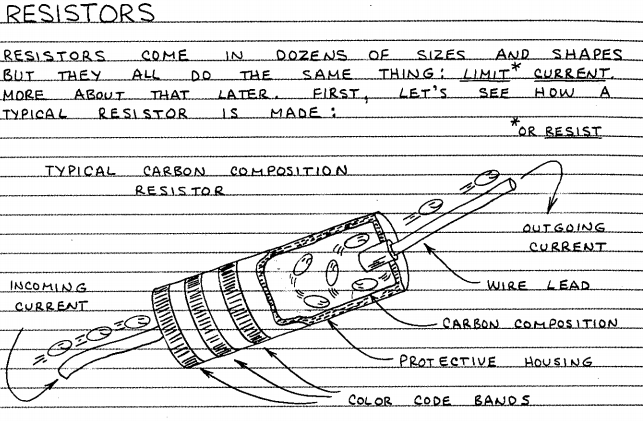
\includegraphics[width=0.75\textwidth]{img/resistor.png}
\end{figure}

      A resistor can be seen here, notice the color bands on the body of the resistor. These are used
      to indicate the resistance value of the part.
      
\begin{figure}[H]
\caption{ A Resistor }
\label{fig:img/resistorirl.jpg}
\centering
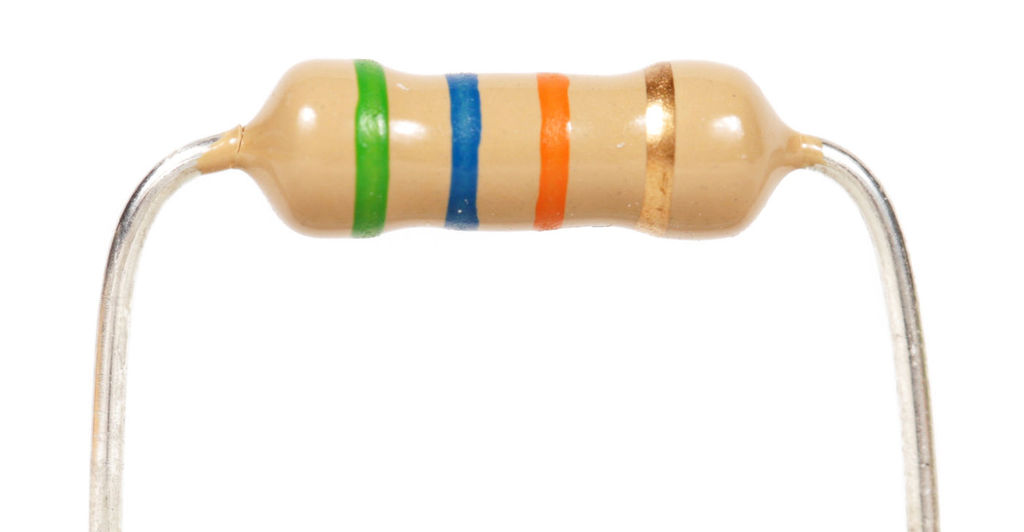
\includegraphics[width=0.3\textwidth]{img/resistorirl.jpg}
\end{figure}

      To find out the value based on the color code, the table below is helpful. The colors are
      mapped to numeric values based on a modified rainbow (Black-Brown-ROYGBIV-White). The value is analogous
      to scientific notation. For a 4 band resistor the first two bands represent the ``a'' in $a\times10^{b}$, the third
      band represents the ``b''. Finally, the fourth band represents the tolerance of the resistor (how accurate the resistance
      is to its rated value). For some applications, there can be a very narrow tolerance for the circuit to work correctly. There are also
      online resistor code calculators that speed things up greatly.
      
\begin{figure}[H]
\caption{ Credit: Forrest M. Mims }
\label{fig:img/codes.png}
\centering
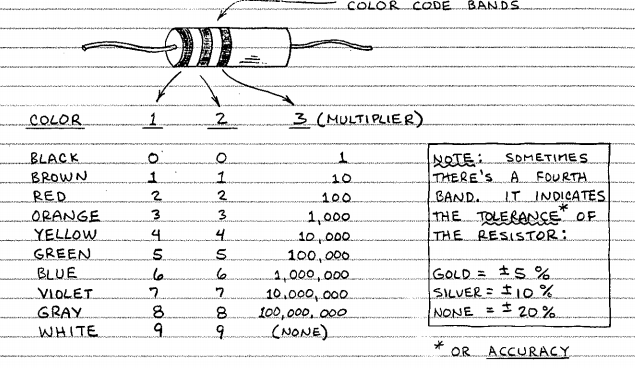
\includegraphics[width=0.75\textwidth]{img/codes.png}
\end{figure}

    


    
                    \subsection{Capacitors}
  
      The next component is the capacitor, it is essentially a storage tank for electricity. In the water model it would
      act like a water tank, where it takes time for the tank to fill and drain. The time to fill the tank is dependent on the rate of the flow (current) as
      well as the size of the tank. Capacitors have a ``capacitance'' value that represents the size of the ``tank'' and it is measured in Farads (F). Typically, this
      value is small. For hobbyist electronics, values are around $10^{-6}F$ which is typically denoted by the Greek letter mu, as in $\mu F$.
      
\begin{figure}[H]
\caption{ Credit: Forrest M. Mims }
\label{fig:img/capacitors.png}
\centering
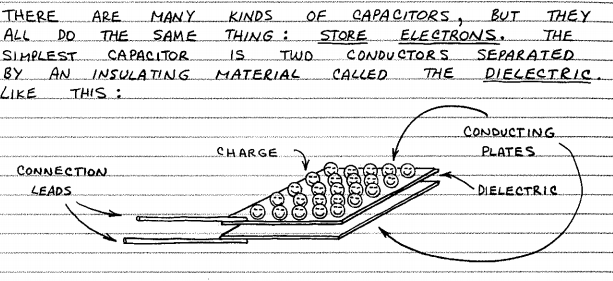
\includegraphics[width=0.75\textwidth]{img/capacitors.png}
\end{figure}

      Below is an image of an Electrolytic Capacitor. Other types of capacitors include ceramic and film. The main difference
      in these capacitors is the range that they operate. Electrolytic capacitors typically have a higher capacitance than ceramic, but Electrolytic caps have the
      consequence of being \textit{polarized}. A polarized component is one that has a positive and negative lead. If the capacitor is connected backwards and there
      is significant voltage it can cause the component to fail, and possible burst. The capacitor will have the polarity indicated on the side. Usually negative lead is labeled,
      additionally, the positive lead will the longer of the two.
      
\begin{figure}[H]
\caption{ An Electrolytic Capacitor }
\label{fig:img/capirl.jpg}
\centering
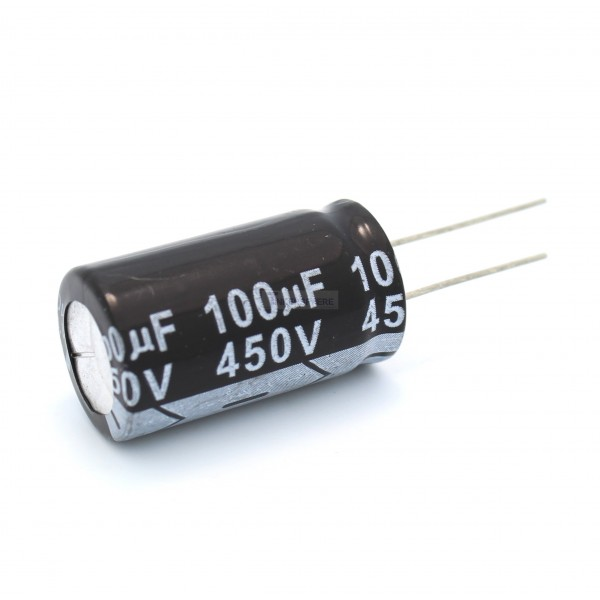
\includegraphics[width=0.3\textwidth]{img/capirl.jpg}
\end{figure}

      By combining a resistor and a capacitor an RC circuit is made. The resistor limits the current into the capacitor which decreases
      the rate is charges by, and therefore creates a delay in voltage. The image below shows the graph of this occurrence. By selecting specific resistor and capacitor
      values the delay time can be set.
      
\begin{figure}[H]
\caption{ Credit: Forrest M. Mims }
\label{fig:img/capcharge.png}
\centering
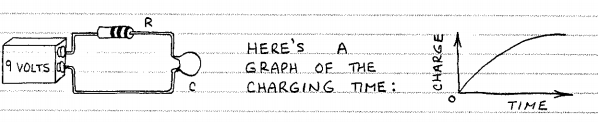
\includegraphics[width=0.75\textwidth]{img/capcharge.png}
\end{figure}

      The circuit we will be building relies on an RC circuit to blink LEDs. Essentially it charges the capacitor through one resistor, and once the voltage
      reaches an upper threshold, it will drain the capacitor through another resistor. Once it drains to a lower threshold it will start over again. This creates
       an oscillation where the on-time and off-time are set by the two resistors. The chip that we will be using is the 555 Timer IC, which handles the logic
       of turing on and off the flow of electricity to the capacitor.
    


    
                    \subsection{Additional Components}
  
      In addition to the basic components here are the other components that will be used
      
\begin{figure}[H]
\caption{ A 5mm LED }
\label{fig:img/LED.jpg}
\centering
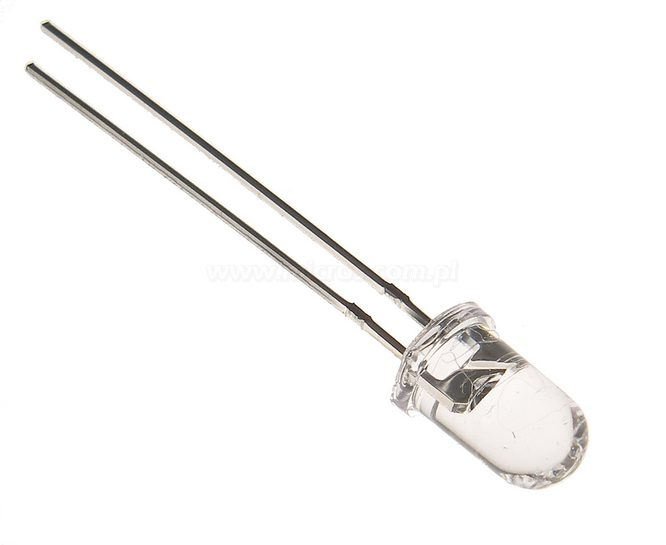
\includegraphics[width=0.3\textwidth]{img/LED.jpg}
\end{figure}

      
\begin{figure}[H]
\caption{ A 555 Timer IC (Integrated Circuit) }
\label{fig:img/555.jpg}
\centering
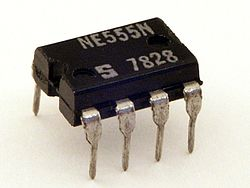
\includegraphics[width=0.3\textwidth]{img/555.jpg}
\end{figure}

      
\begin{figure}[H]
\caption{ An IC Socket }
\label{fig:img/IC_Socket.jpg}
\centering
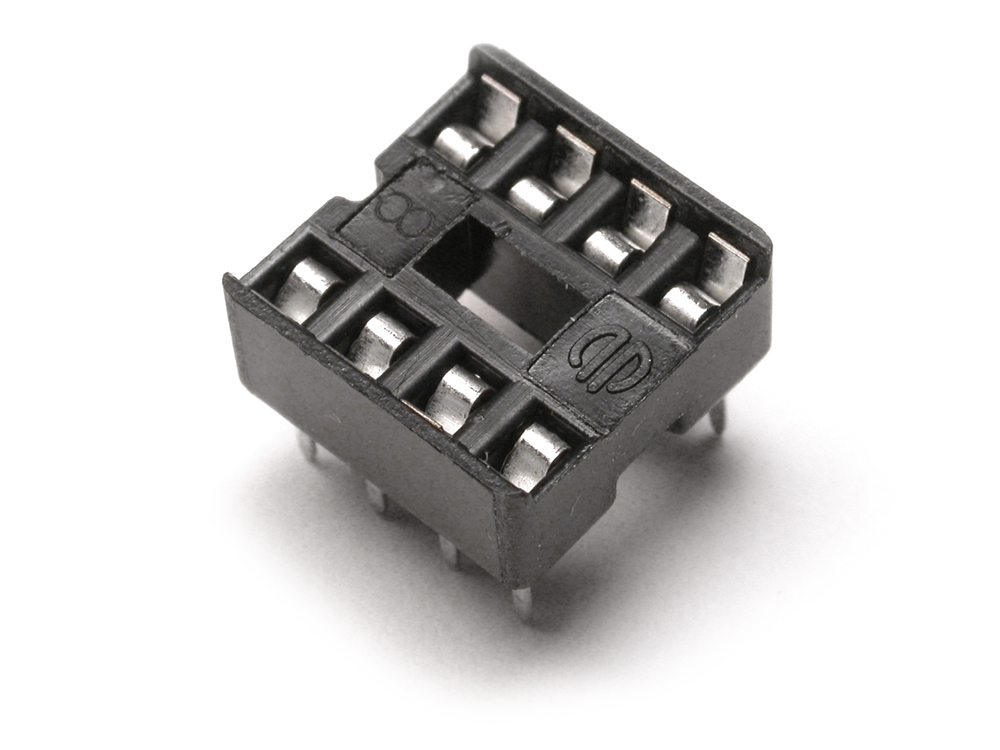
\includegraphics[width=0.3\textwidth]{img/IC_Socket.jpg}
\end{figure}

    


  


  
              \section{Soldering}
  
    Here are all the required parts for the workshop,
    
    \begin{enumerate}
  
      \item 9V battery snap
      \item Printed Circuit Board
      \item $10\mu F$ Electrolytic Capacitor
      \item 555 Timer IC
      \item Two LEDs of any color
      \item $1k\Omega$ resistor
      \item $10k\Omega$ resistor
      \item 2 $620\Omega$ resistor
      \item 8 pin IC socket(not pictured)
    
  \end{enumerate}

    
\begin{figure}[H]
\caption{ Required Items }
\label{fig:img/0002.jpg}
\centering
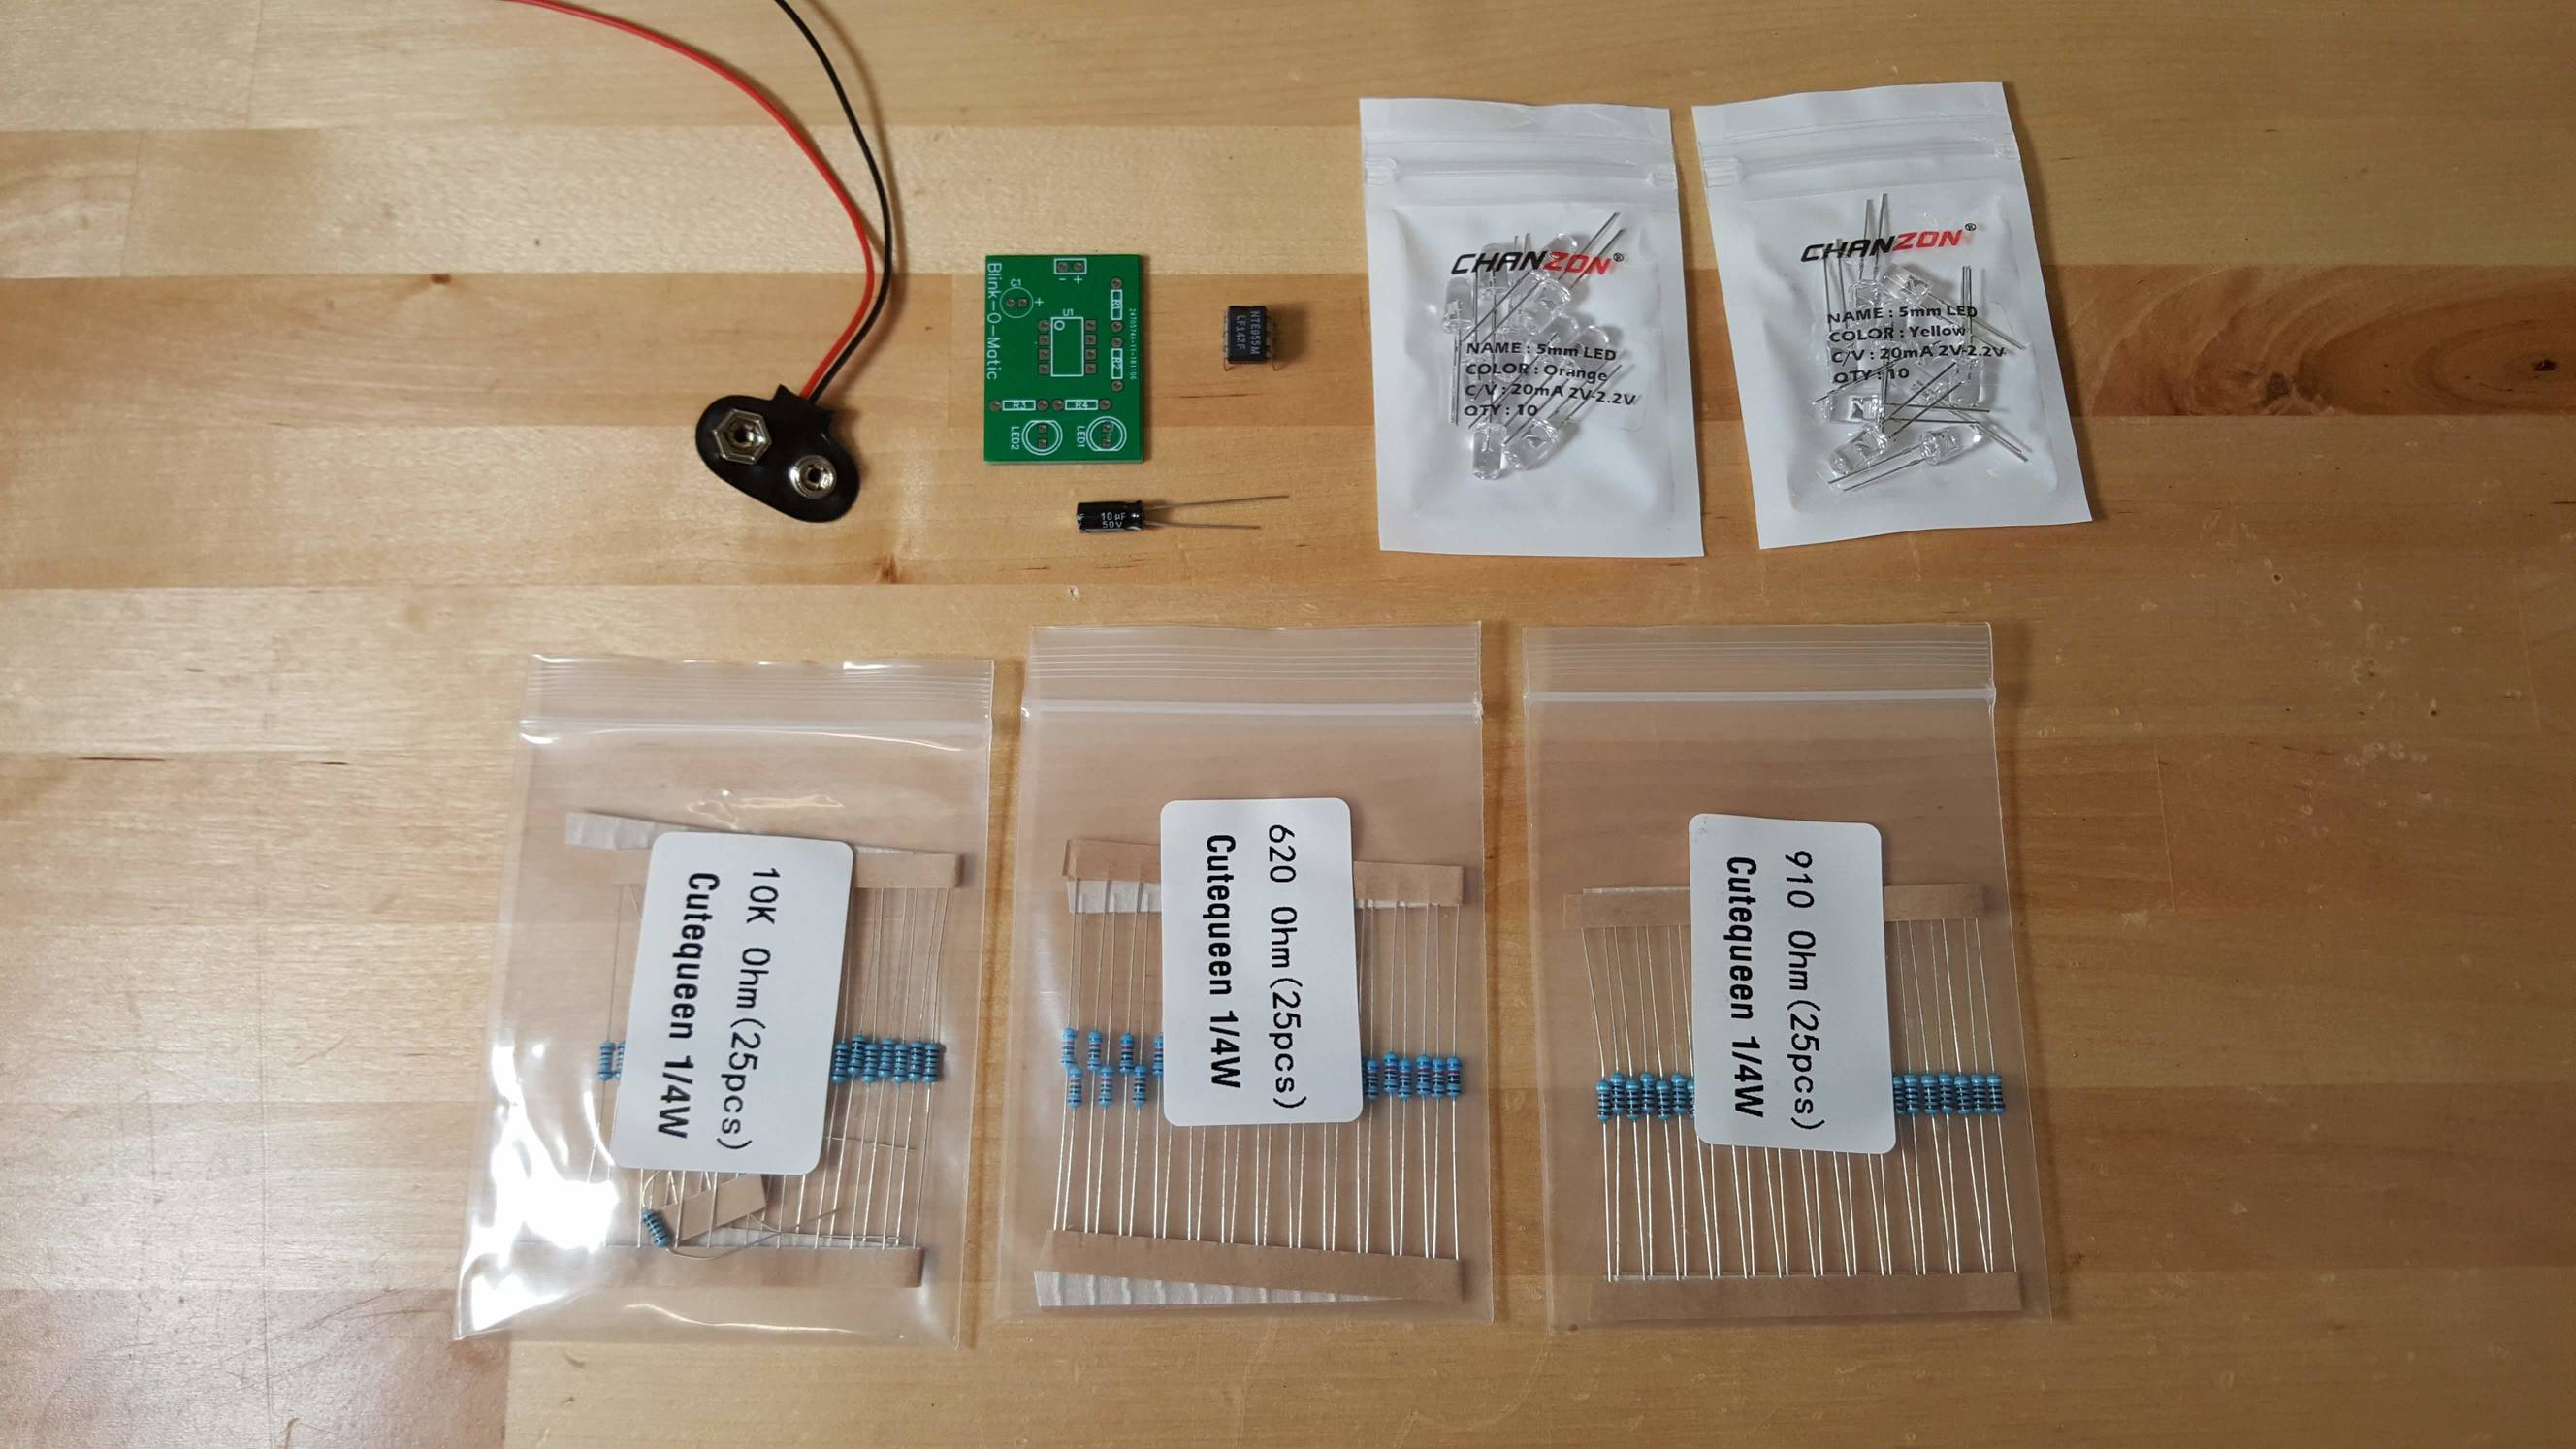
\includegraphics[width=0.75\textwidth]{img/0002.jpg}
\end{figure}

    Additionally, A Soldering Iron, Solder, and a possibly a circuit board vice (to hold the board) are required.
    
\begin{figure}[H]
\caption{ Tools }
\label{fig:img/0004.jpg}
\centering
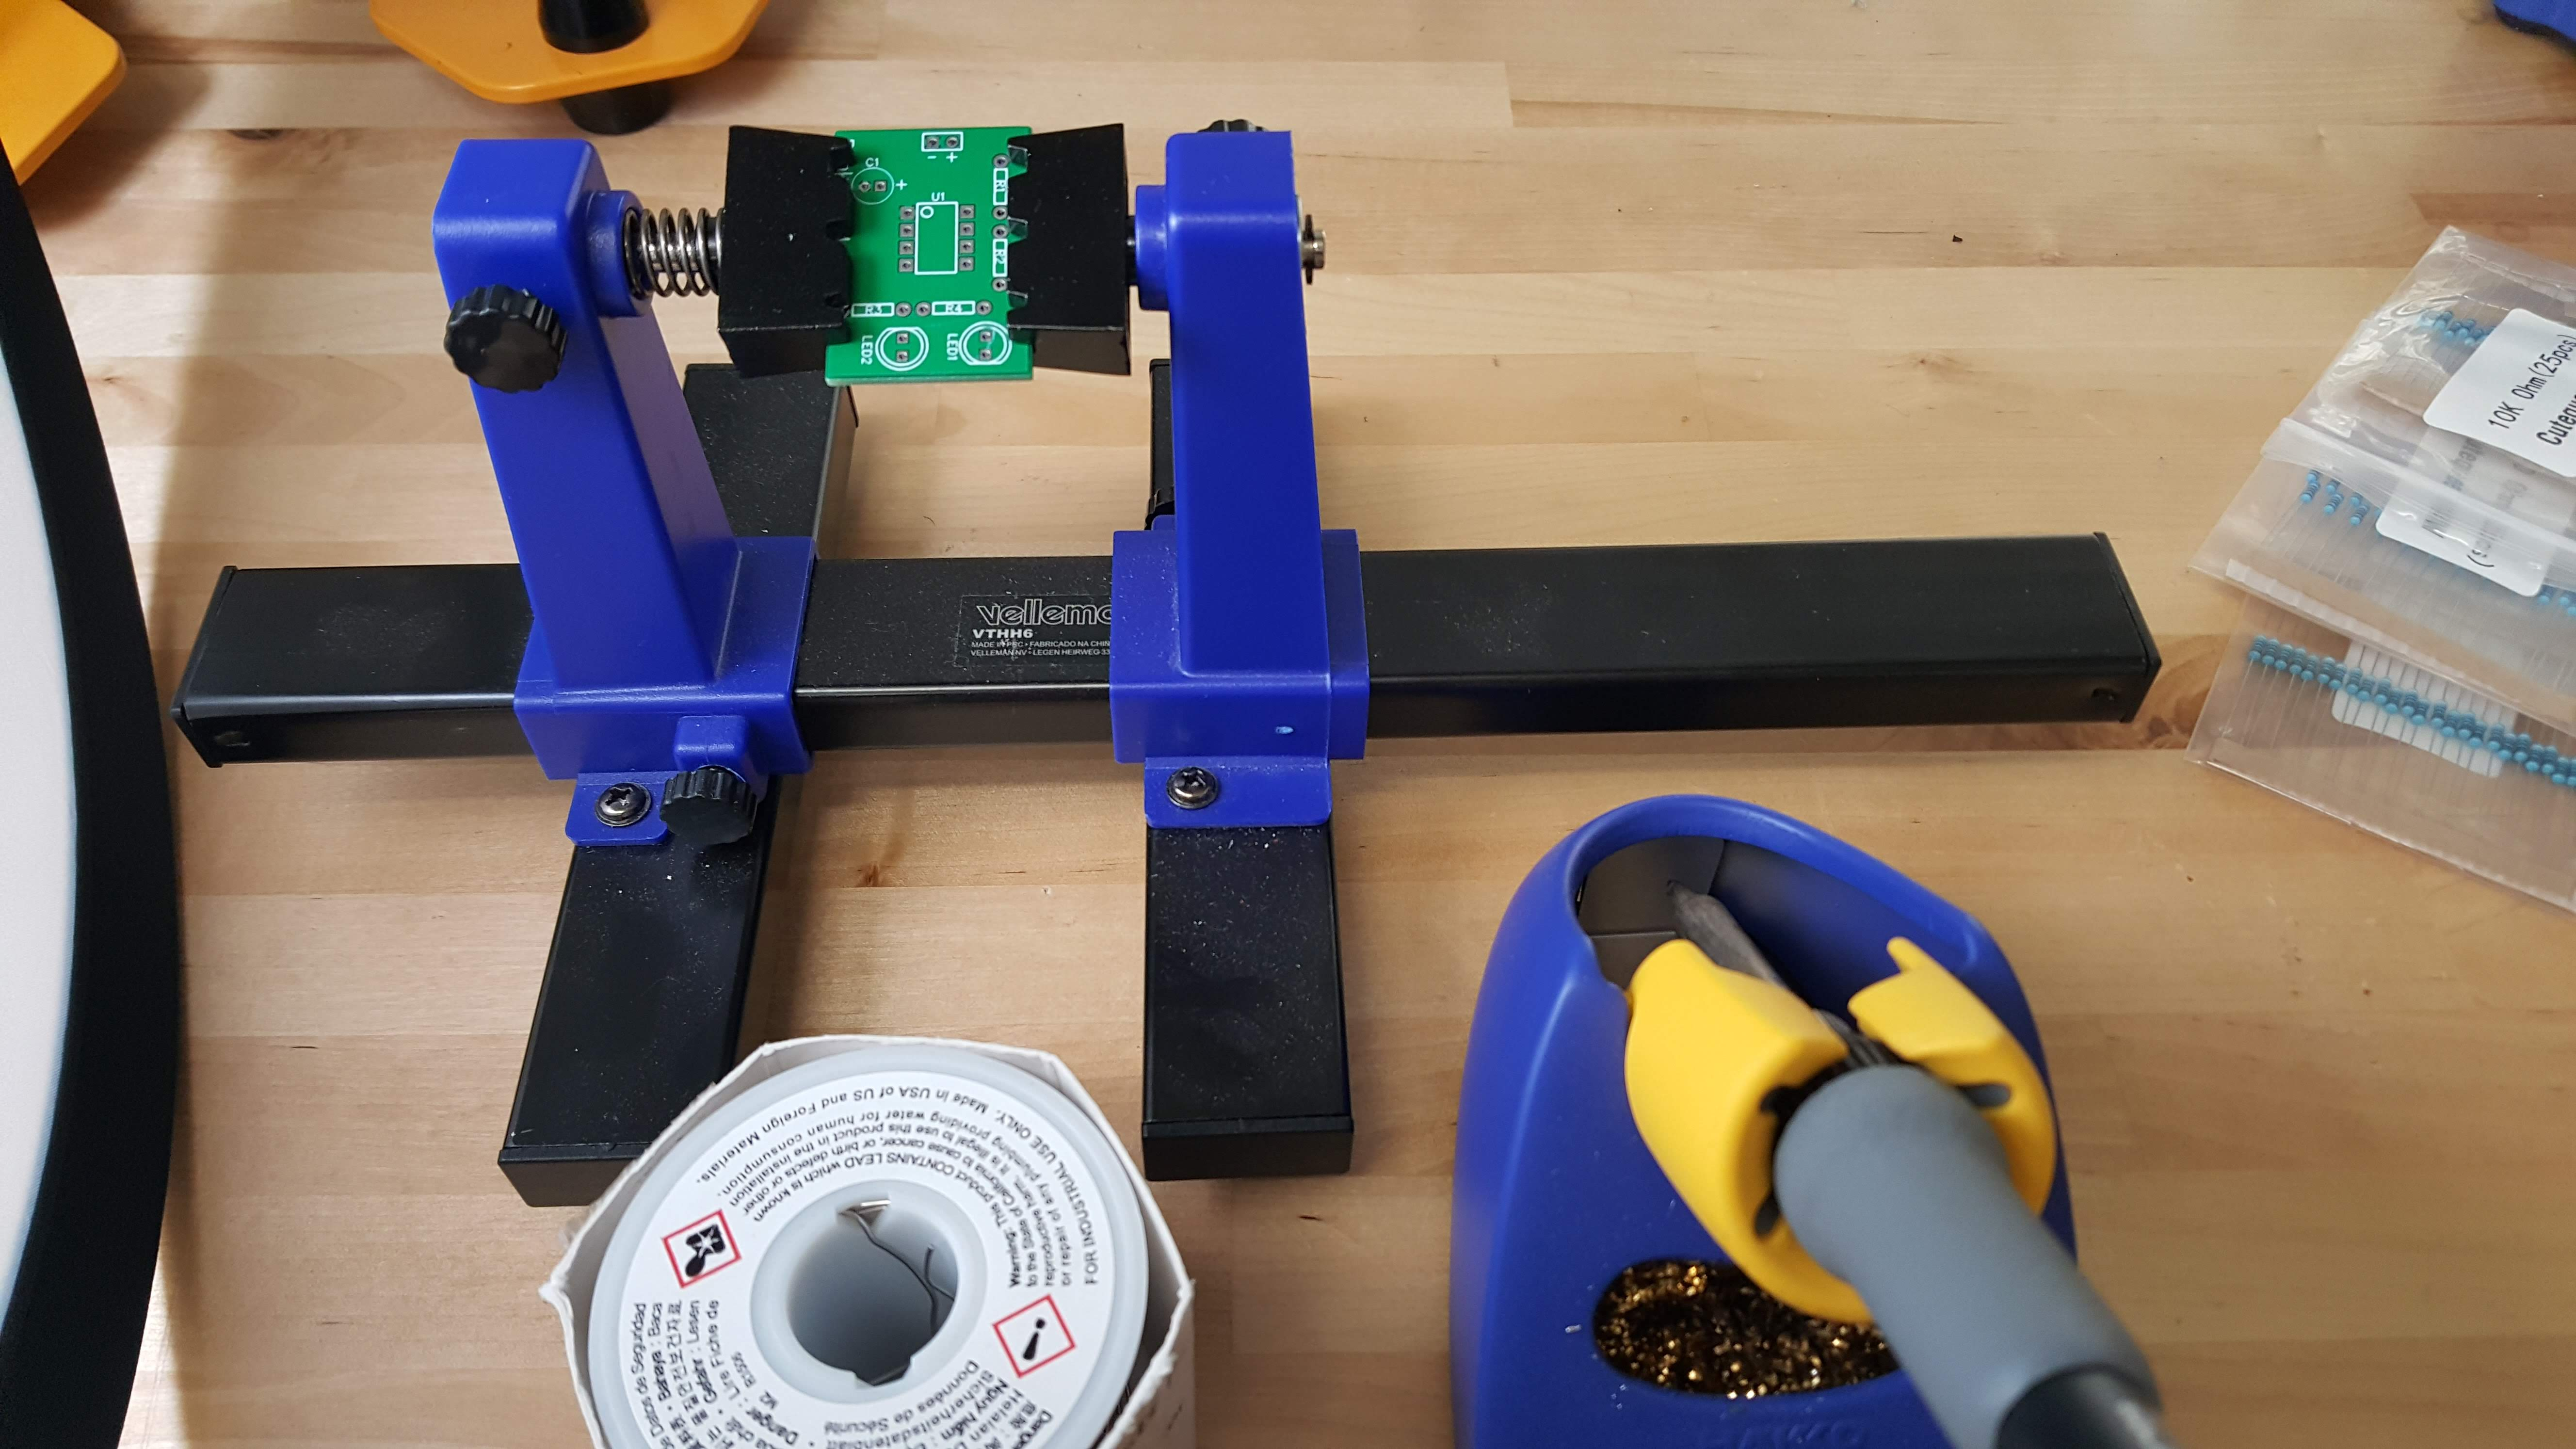
\includegraphics[width=0.75\textwidth]{img/0004.jpg}
\end{figure}

    
\begin{figure}[H]
\caption{ Circuit Schematic for the kit }
\label{fig:img/circuit.png}
\centering
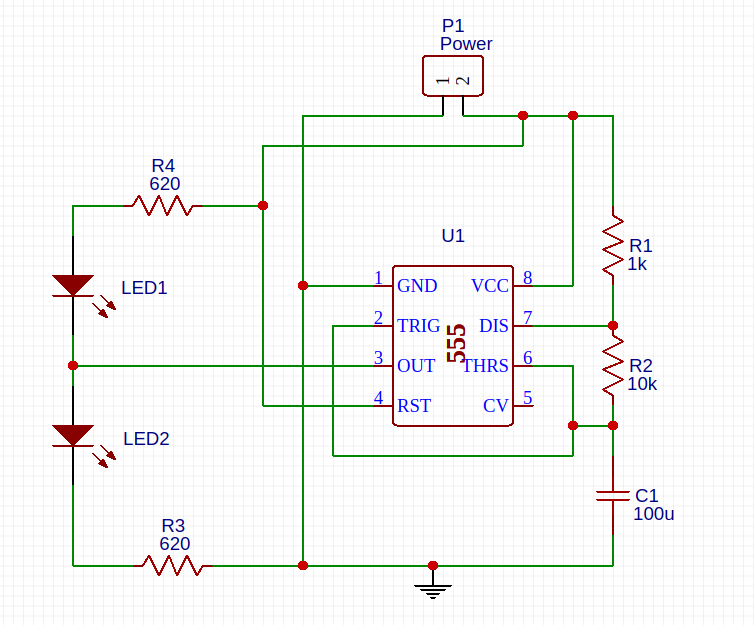
\includegraphics[width=0.75\textwidth]{img/circuit.png}
\end{figure}

    
    \begin{enumerate}
  
      \item 
        
    \begin{enumerate}
  
          \item 
        Typically, the best order to place components is in the order of shortest to tallest. We will start with the resistors. The first two resistor we will place
        are the $620\Omega$ resistors (R3, and R4). Before placing the resistors, bend the leads like this:
        
\begin{figure}[H]
\caption{ Resistor After Bending }
\label{fig:img/0008.jpg}
\centering
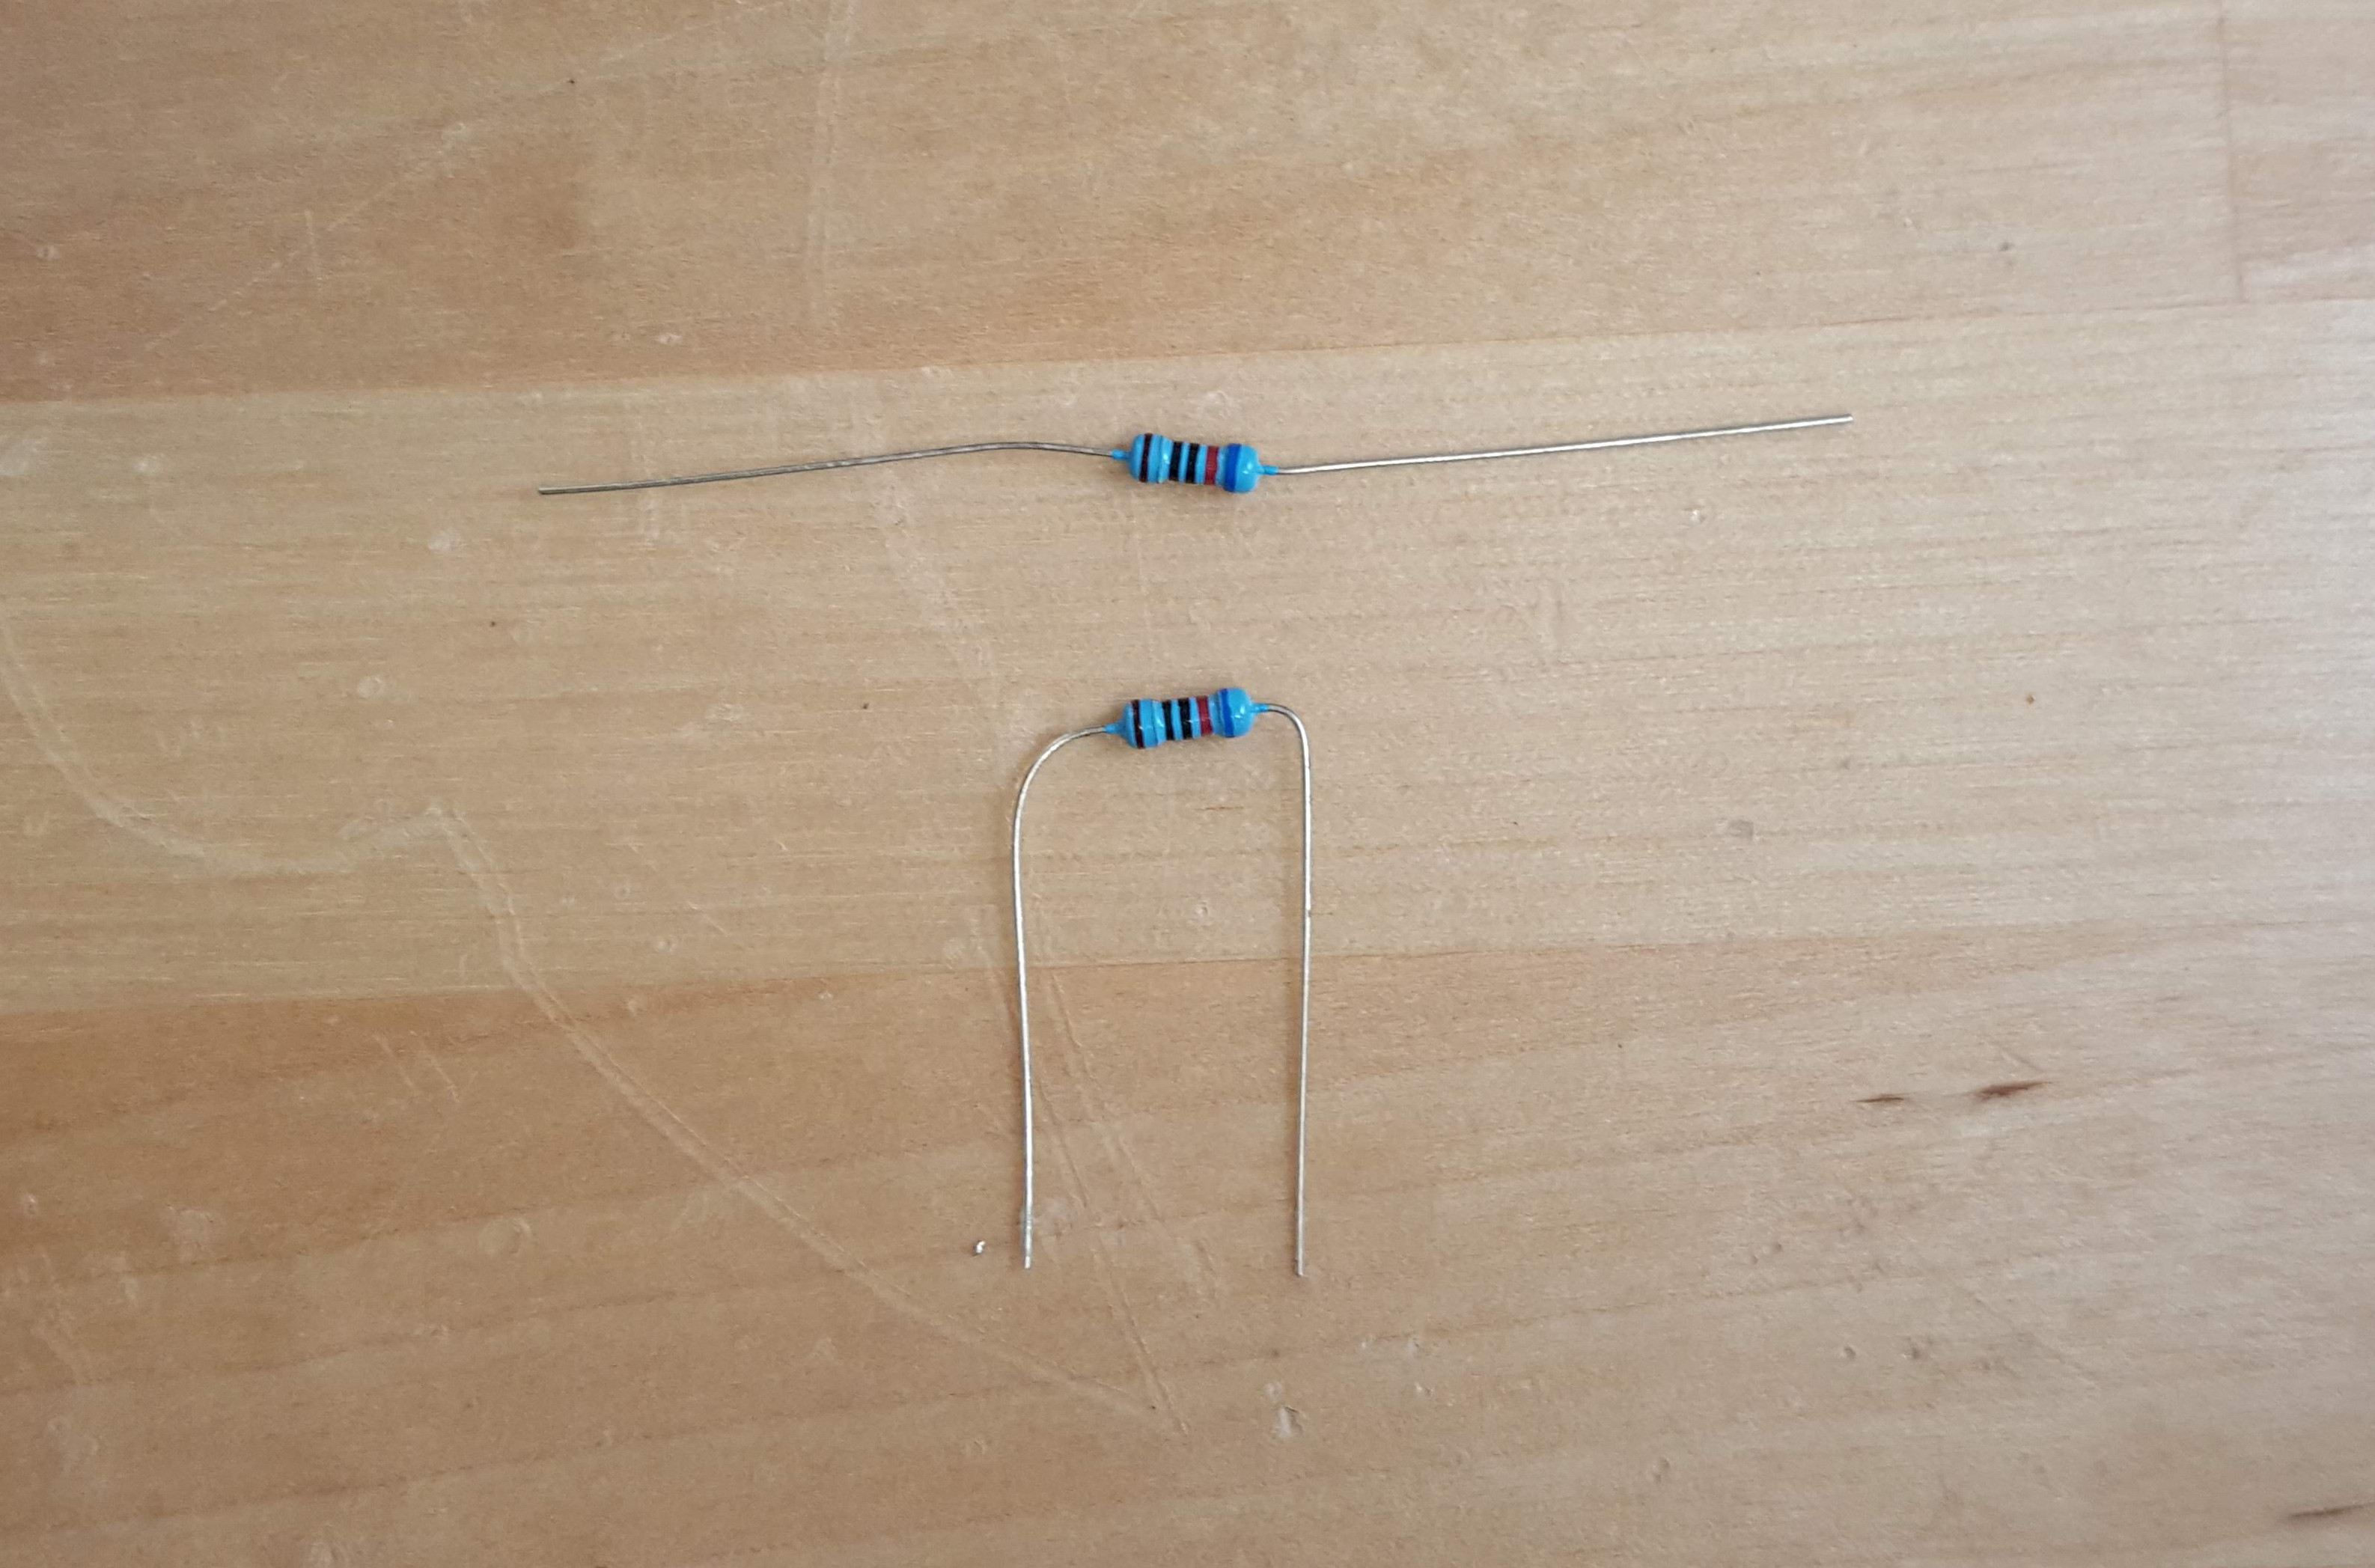
\includegraphics[width=0.75\textwidth]{img/0008.jpg}
\end{figure}

        \item 
        Once bent, these will go in the place of R3, and R4. They are inserted into the holes like in the image below.

        \textbf{Note:} On this circuit board the holes are a little too close together, making it difficult to position
         them flat. For the best results, the resistors
        should lay evenly and a flat to the board.
        
\begin{figure}[H]
\caption{ R3 and R4 Placed on the Board }
\label{fig:img/0005.jpg}
\centering
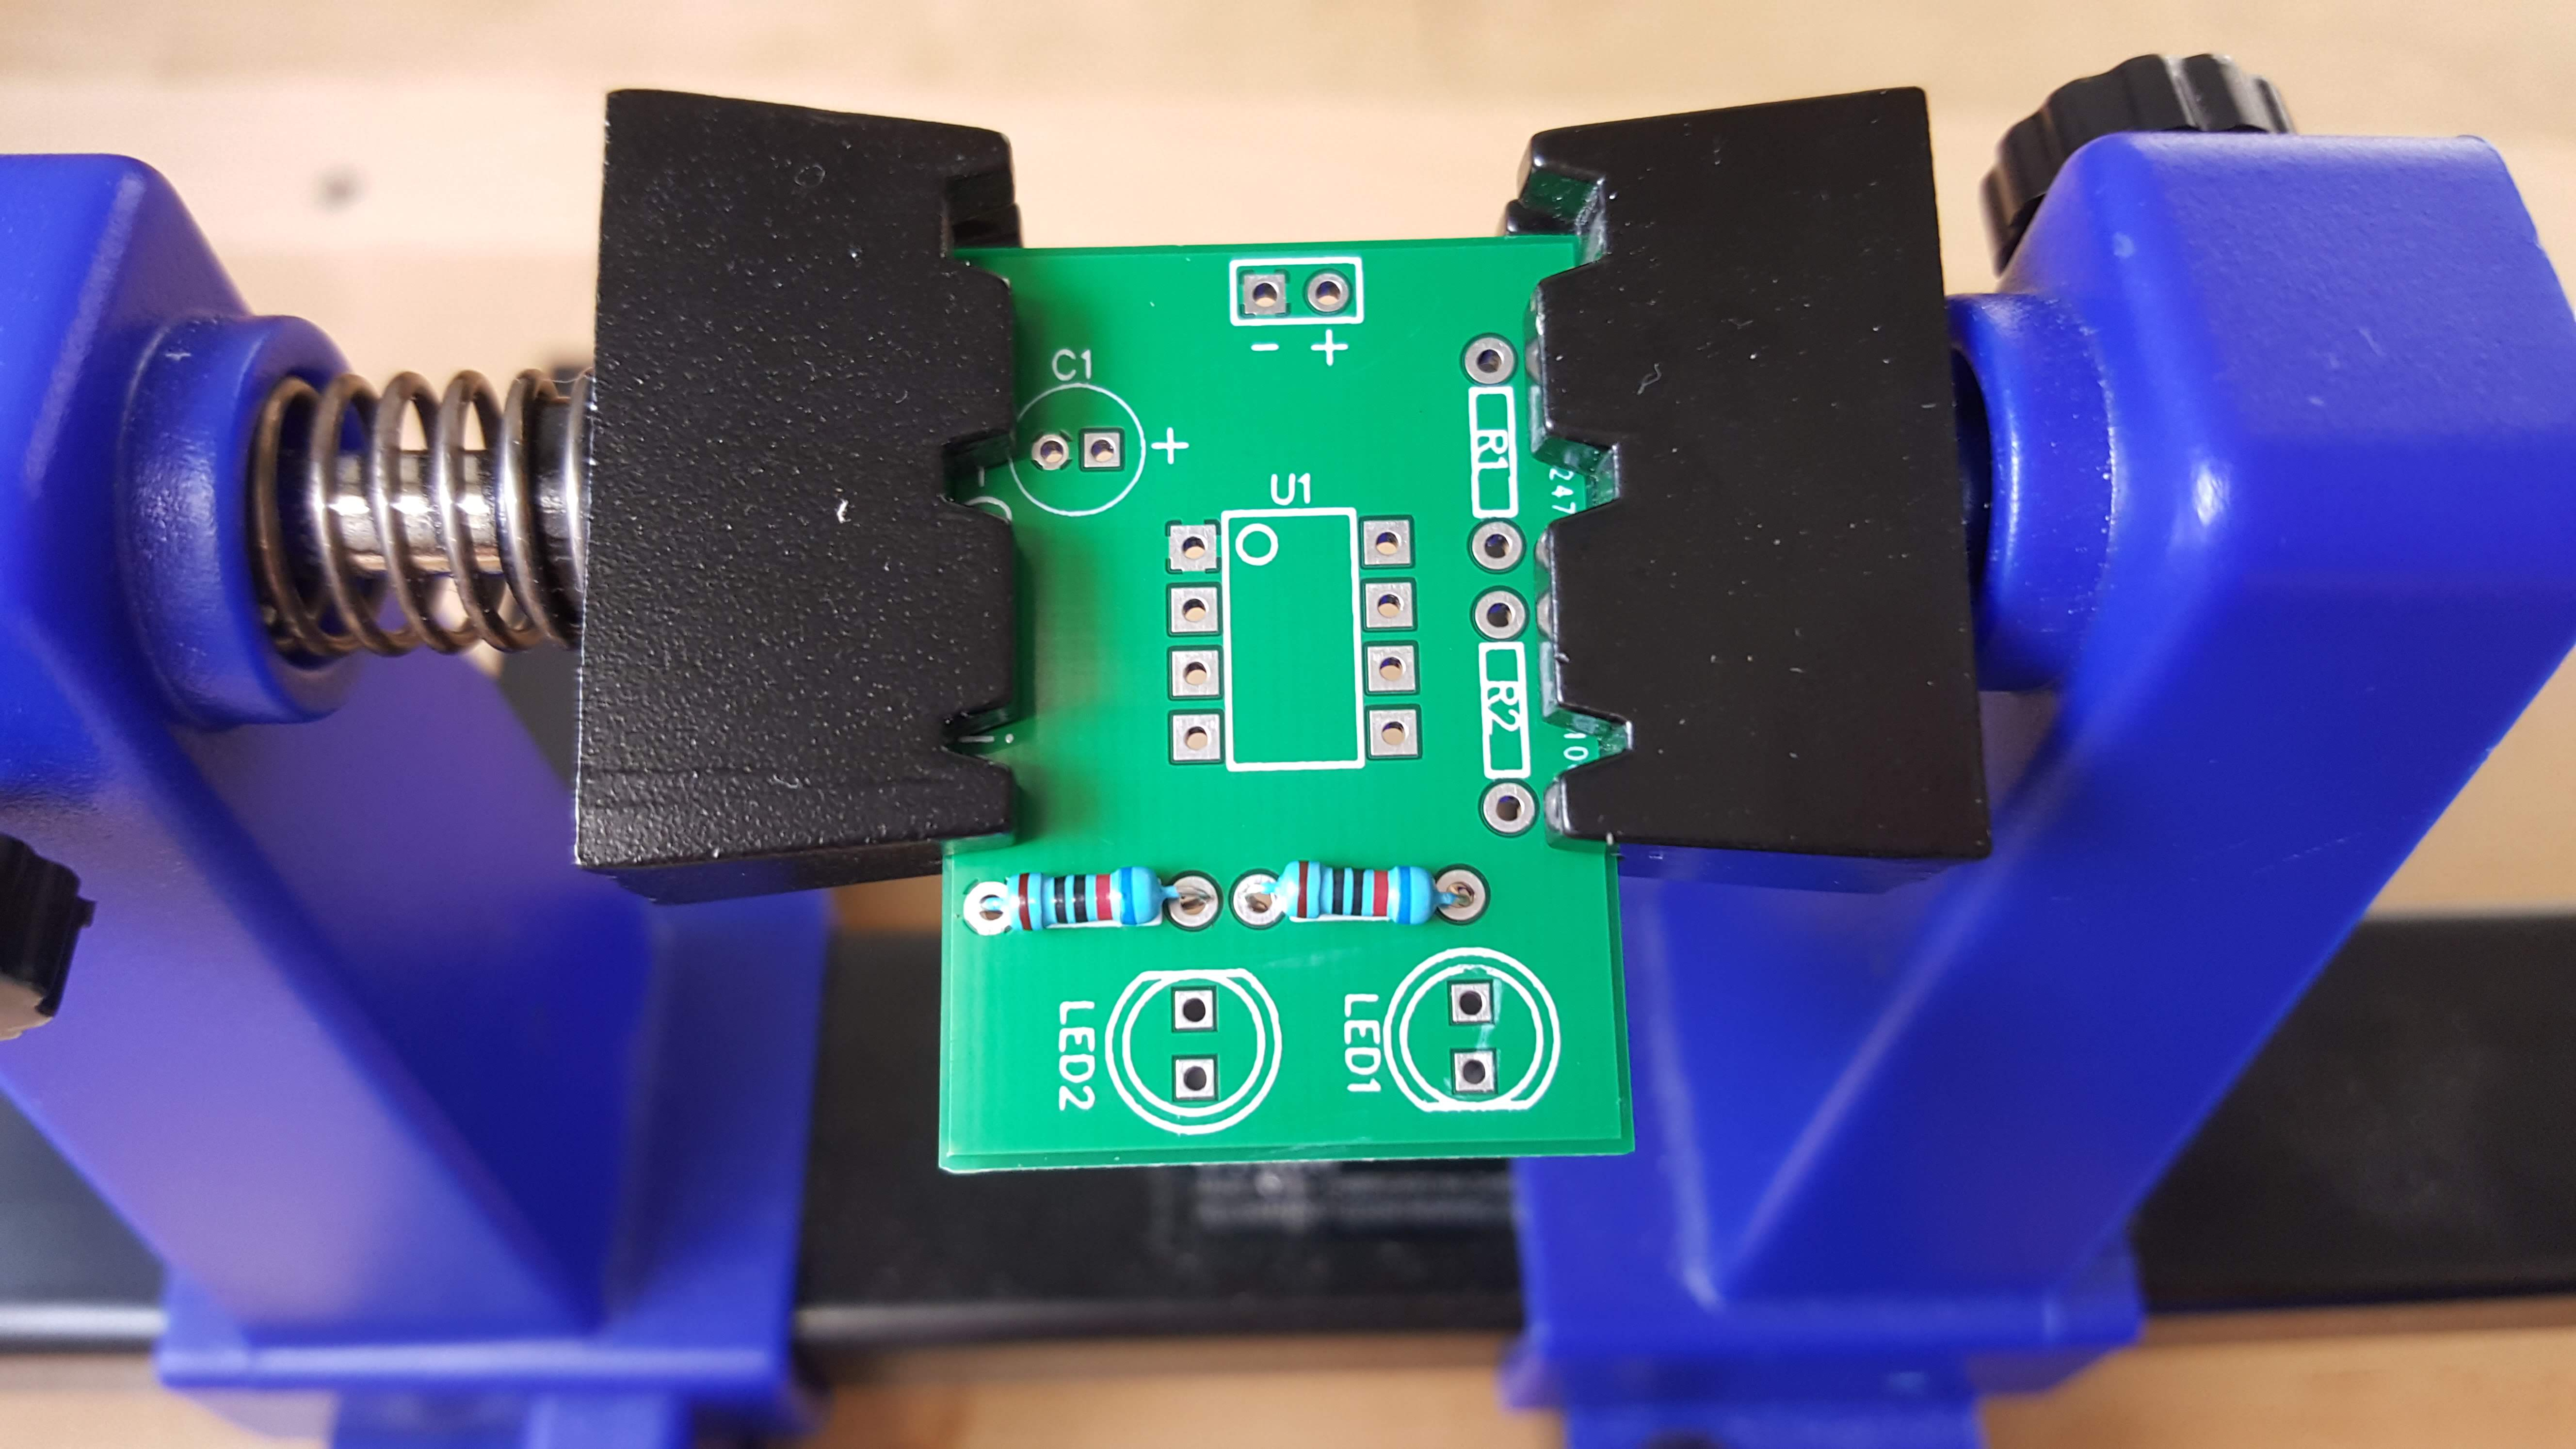
\includegraphics[width=0.75\textwidth]{img/0005.jpg}
\end{figure}

        
\begin{figure}[H]
\caption{ R3 and R4 Placed on the Board (viewed from the bottom side) }
\label{fig:img/0007.jpg}
\centering
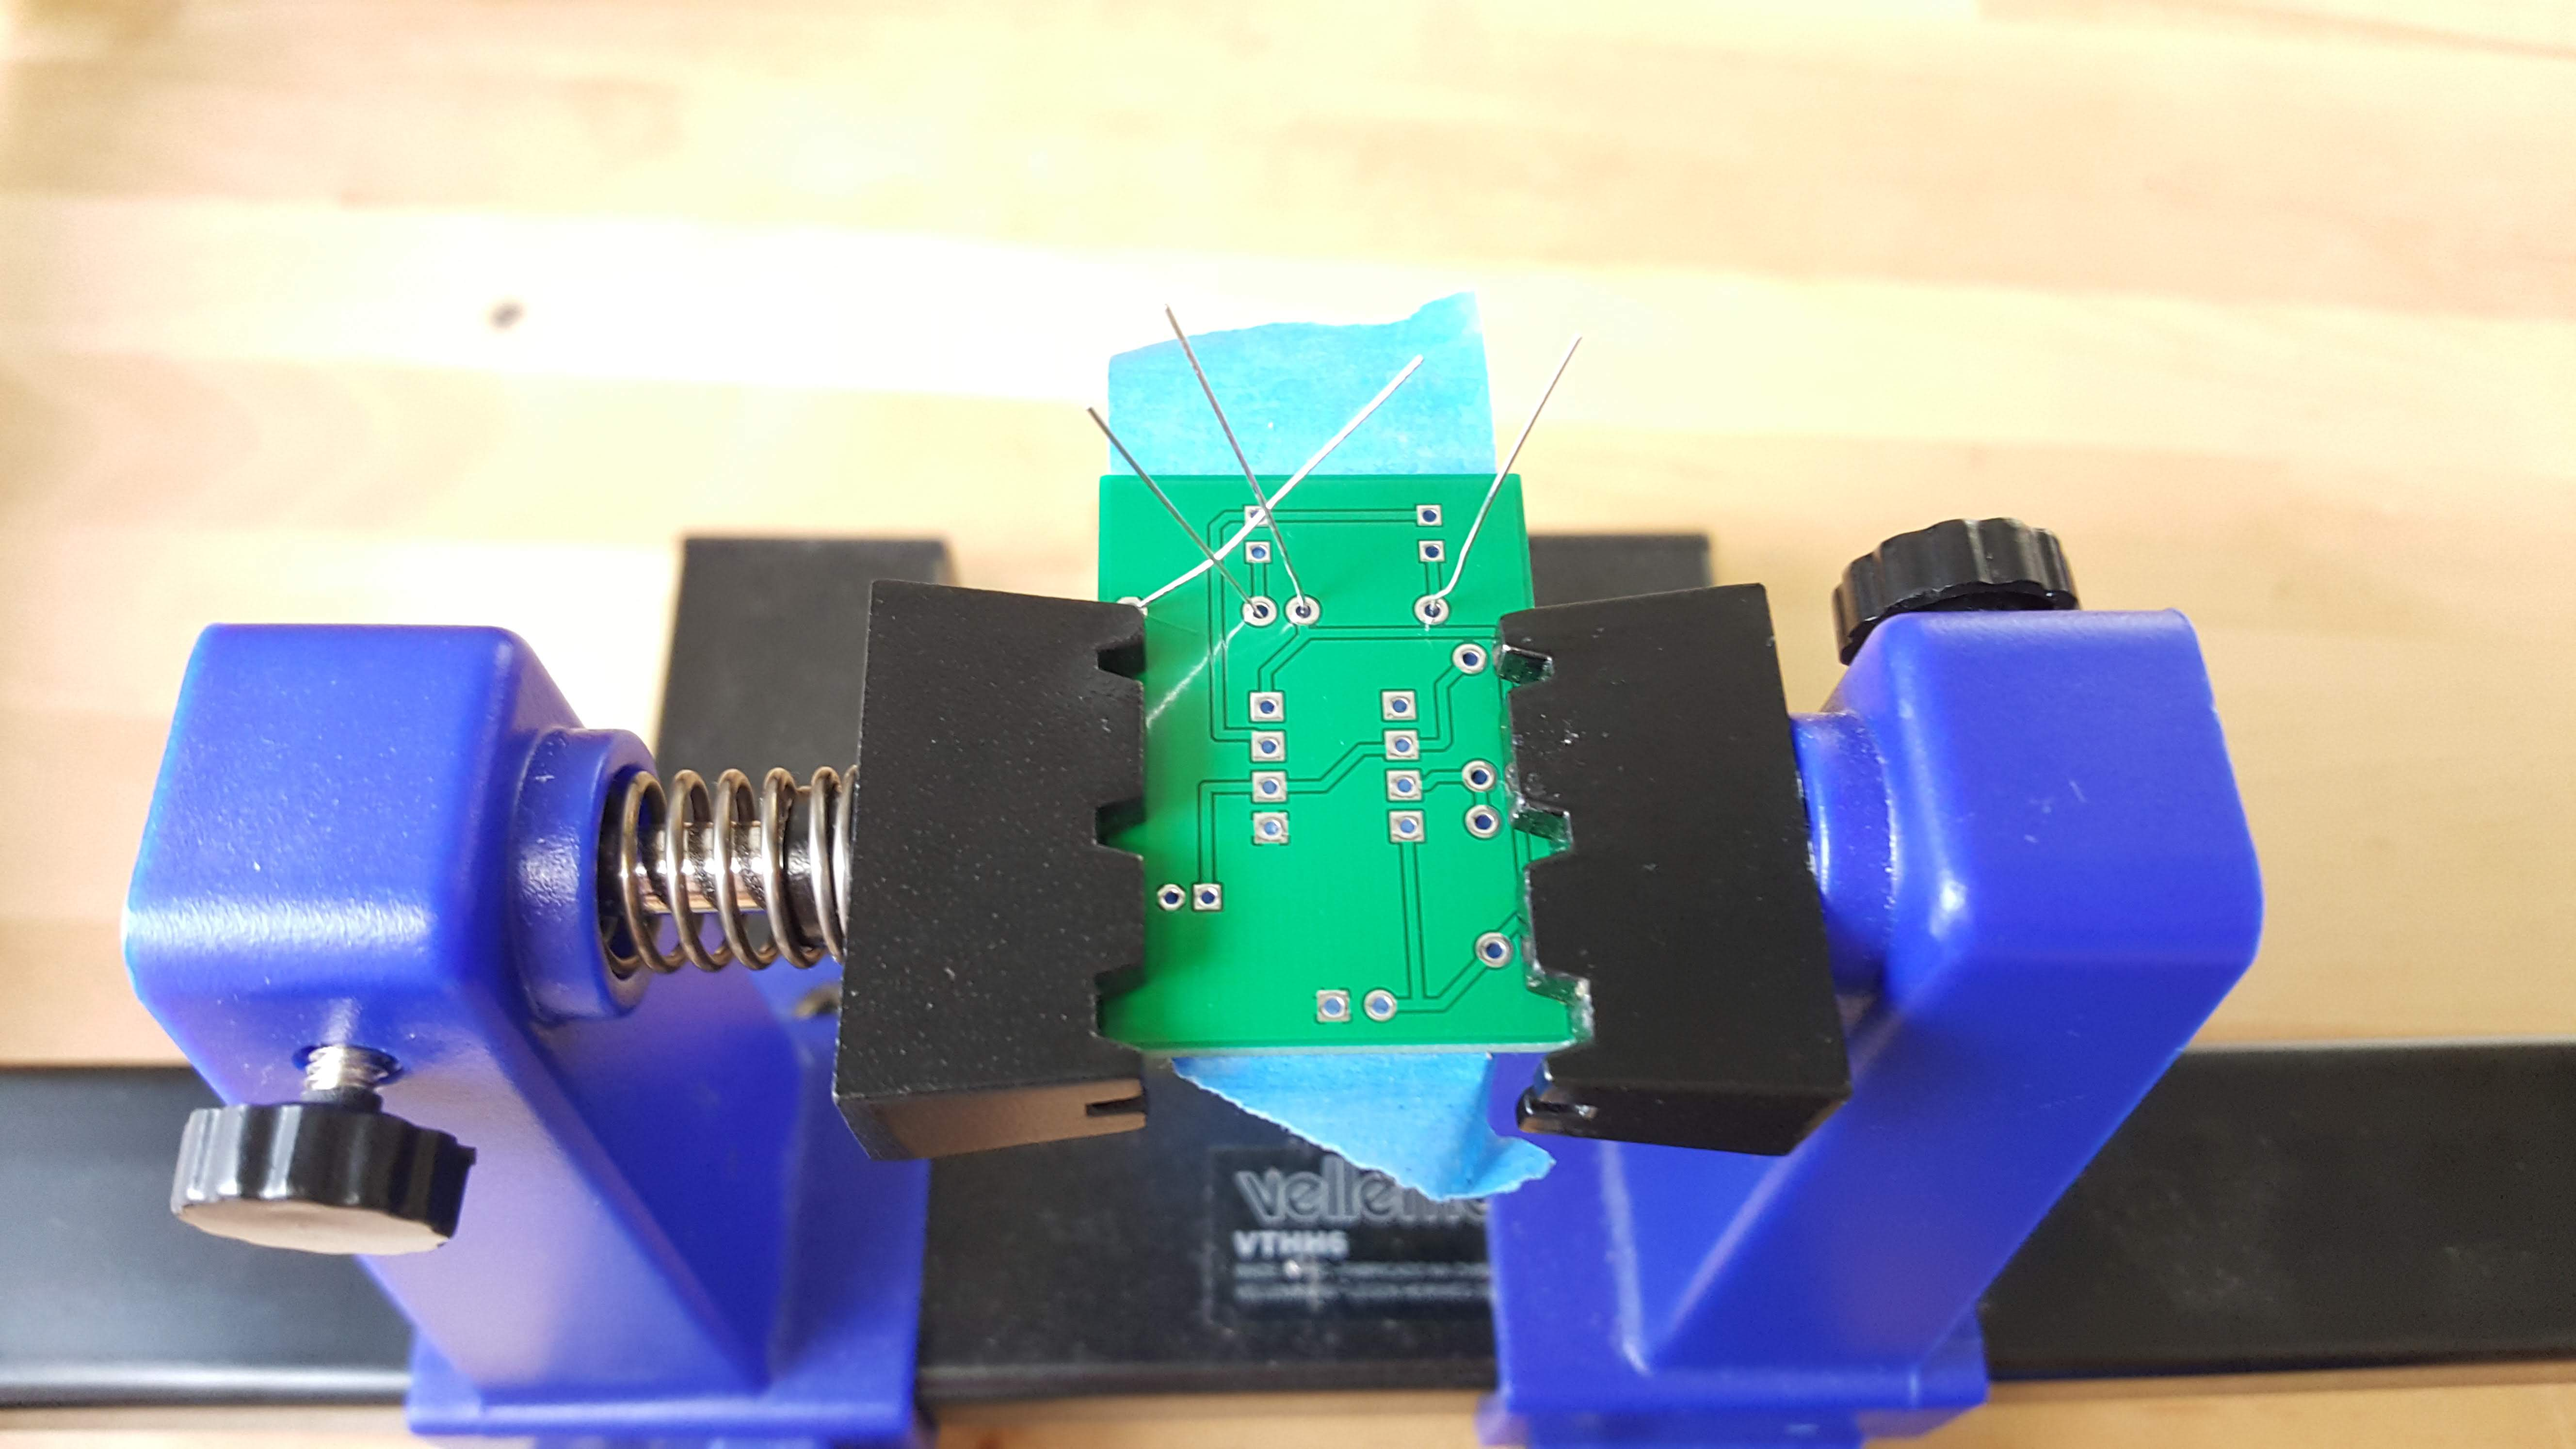
\includegraphics[width=0.75\textwidth]{img/0007.jpg}
\end{figure}

        \item 
        It helps to secure the components with a bit of tape to ensure they stay flat to the board while soldering.
        
\begin{figure}[H]
\caption{ Tape Added to Secure Components }
\label{fig:img/0006.jpg}
\centering
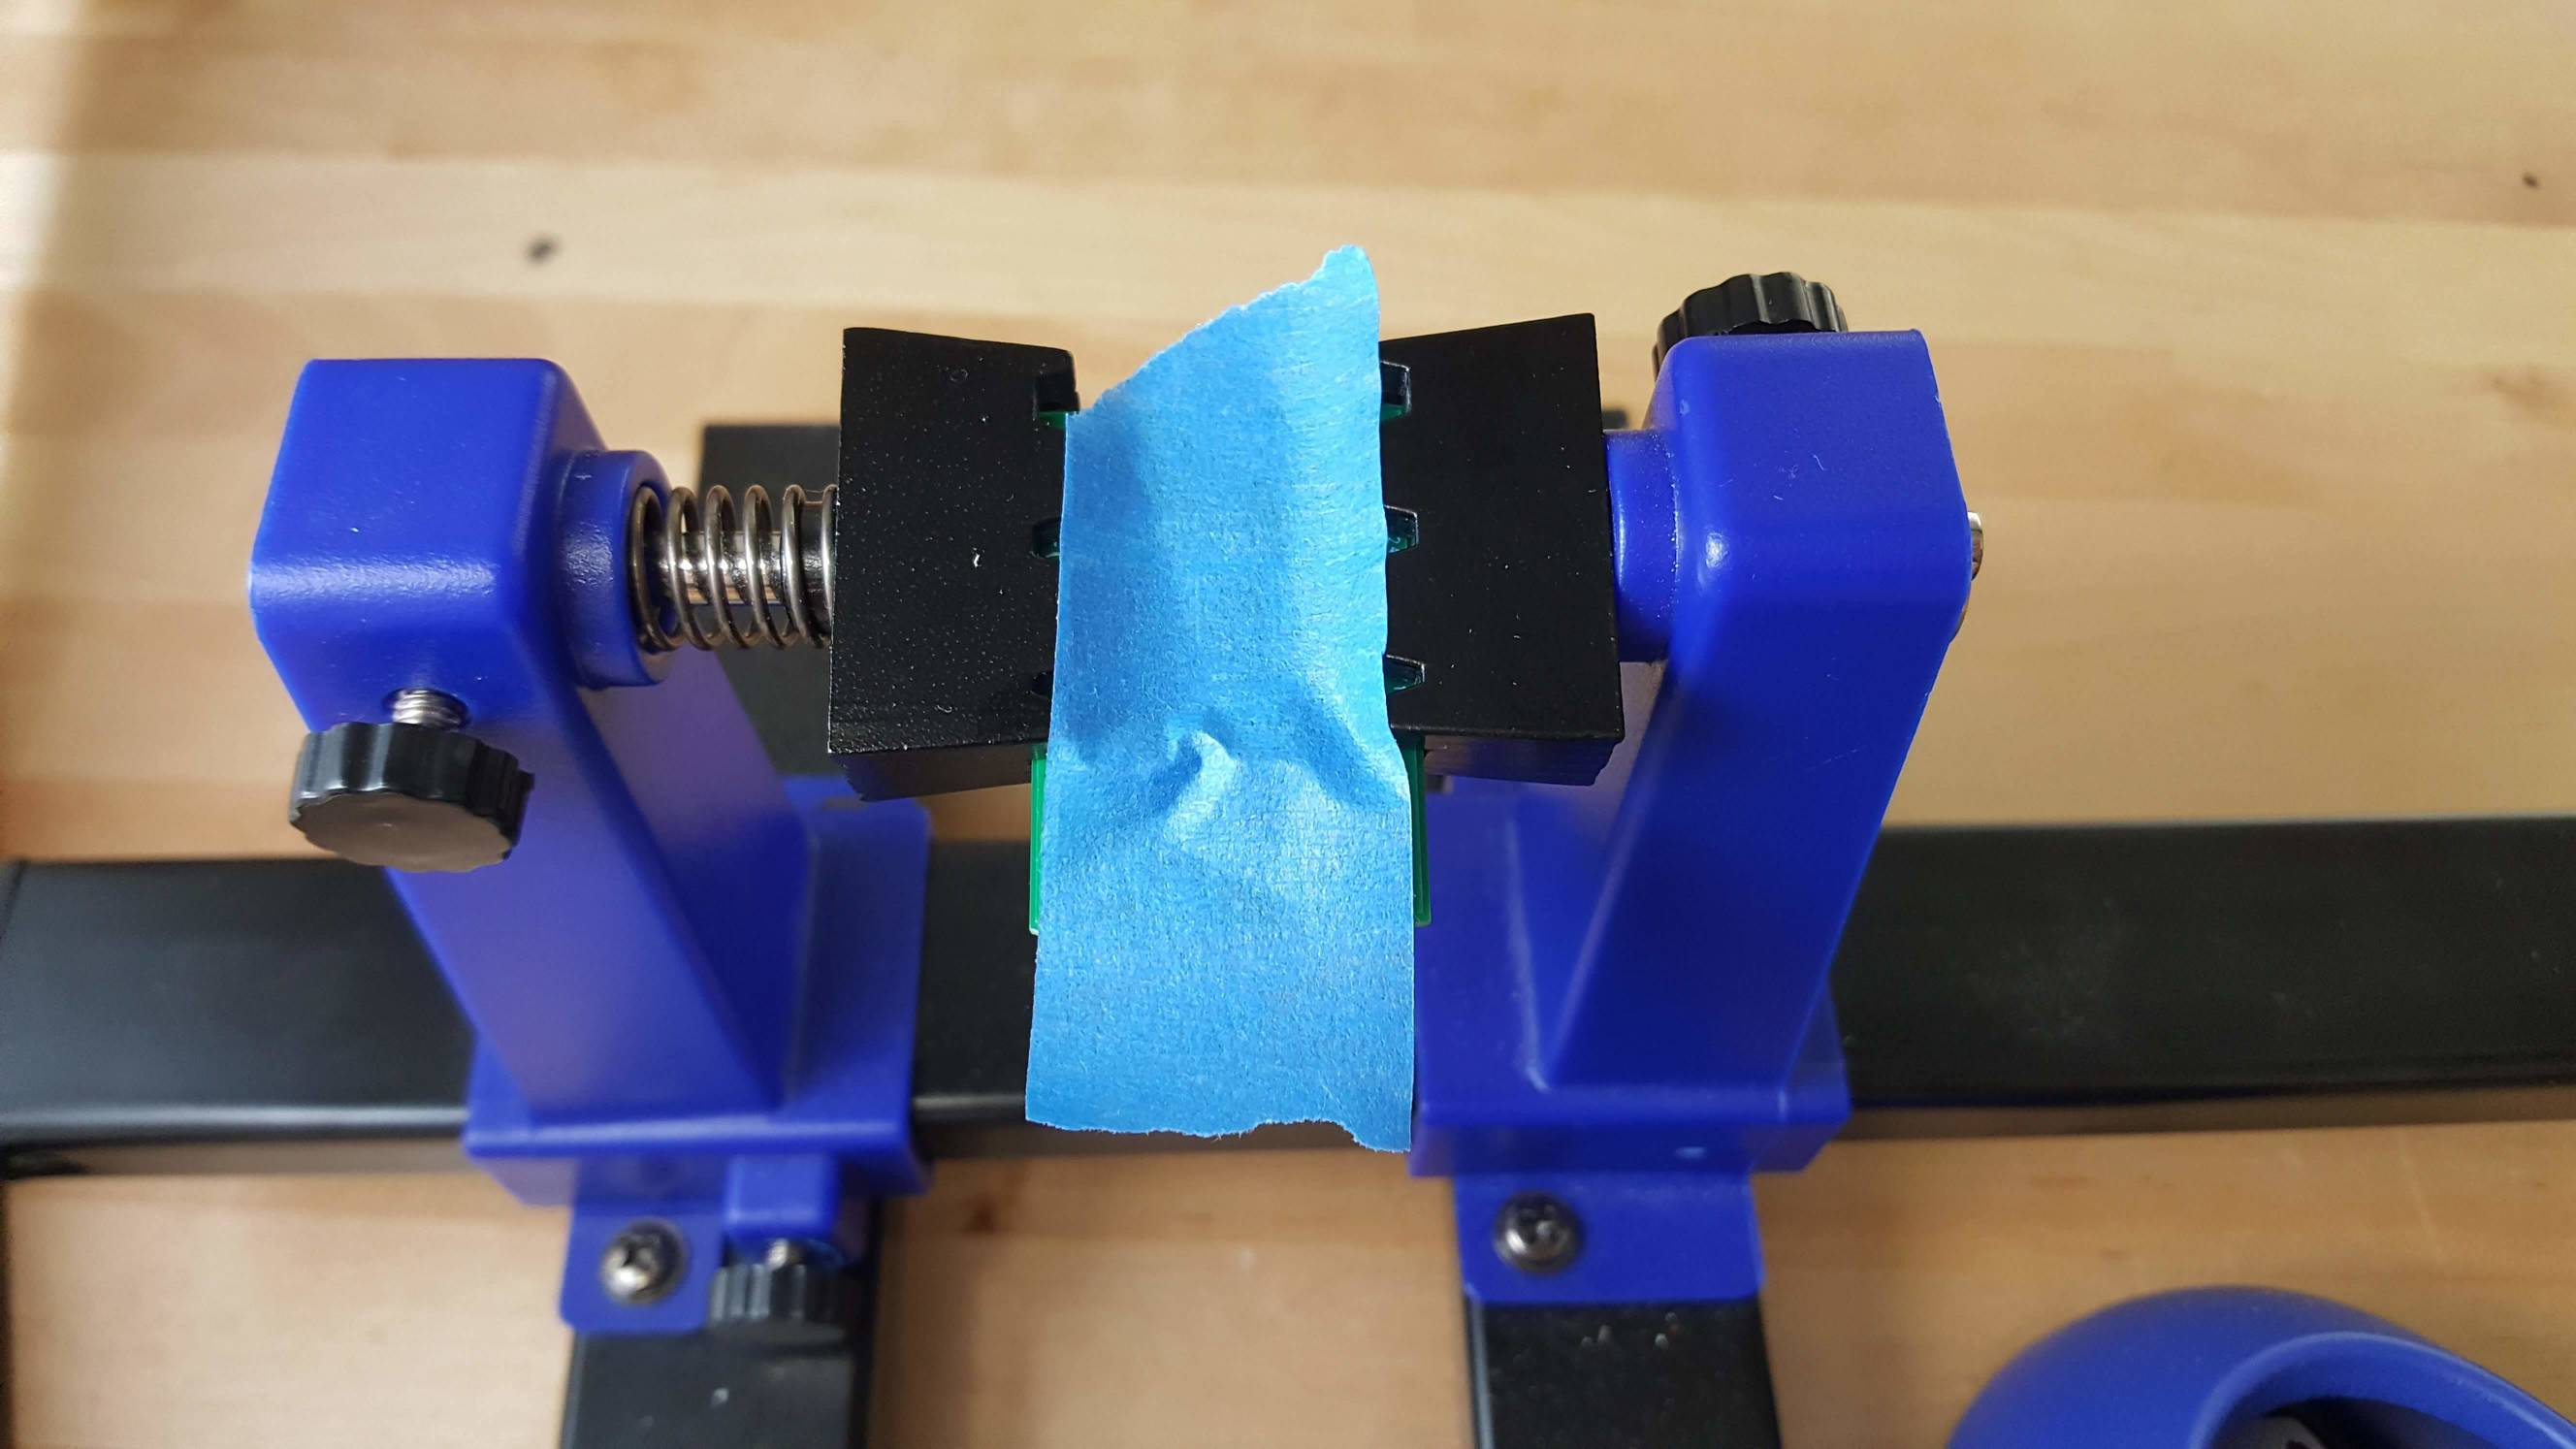
\includegraphics[width=0.75\textwidth]{img/0006.jpg}
\end{figure}

        
  \end{enumerate}

      \item 
      To begin soldering, the iron should be turned on and allowed to heat. When
      ready, apply some solder to the tip of the iron (tinning the iron). Then use the brass
      wool or damp sponge on the stand to clean the tip.
      
\begin{figure}[H]
\caption{ Applying Solder to the Tip }
\label{fig:img/0009.jpg}
\centering
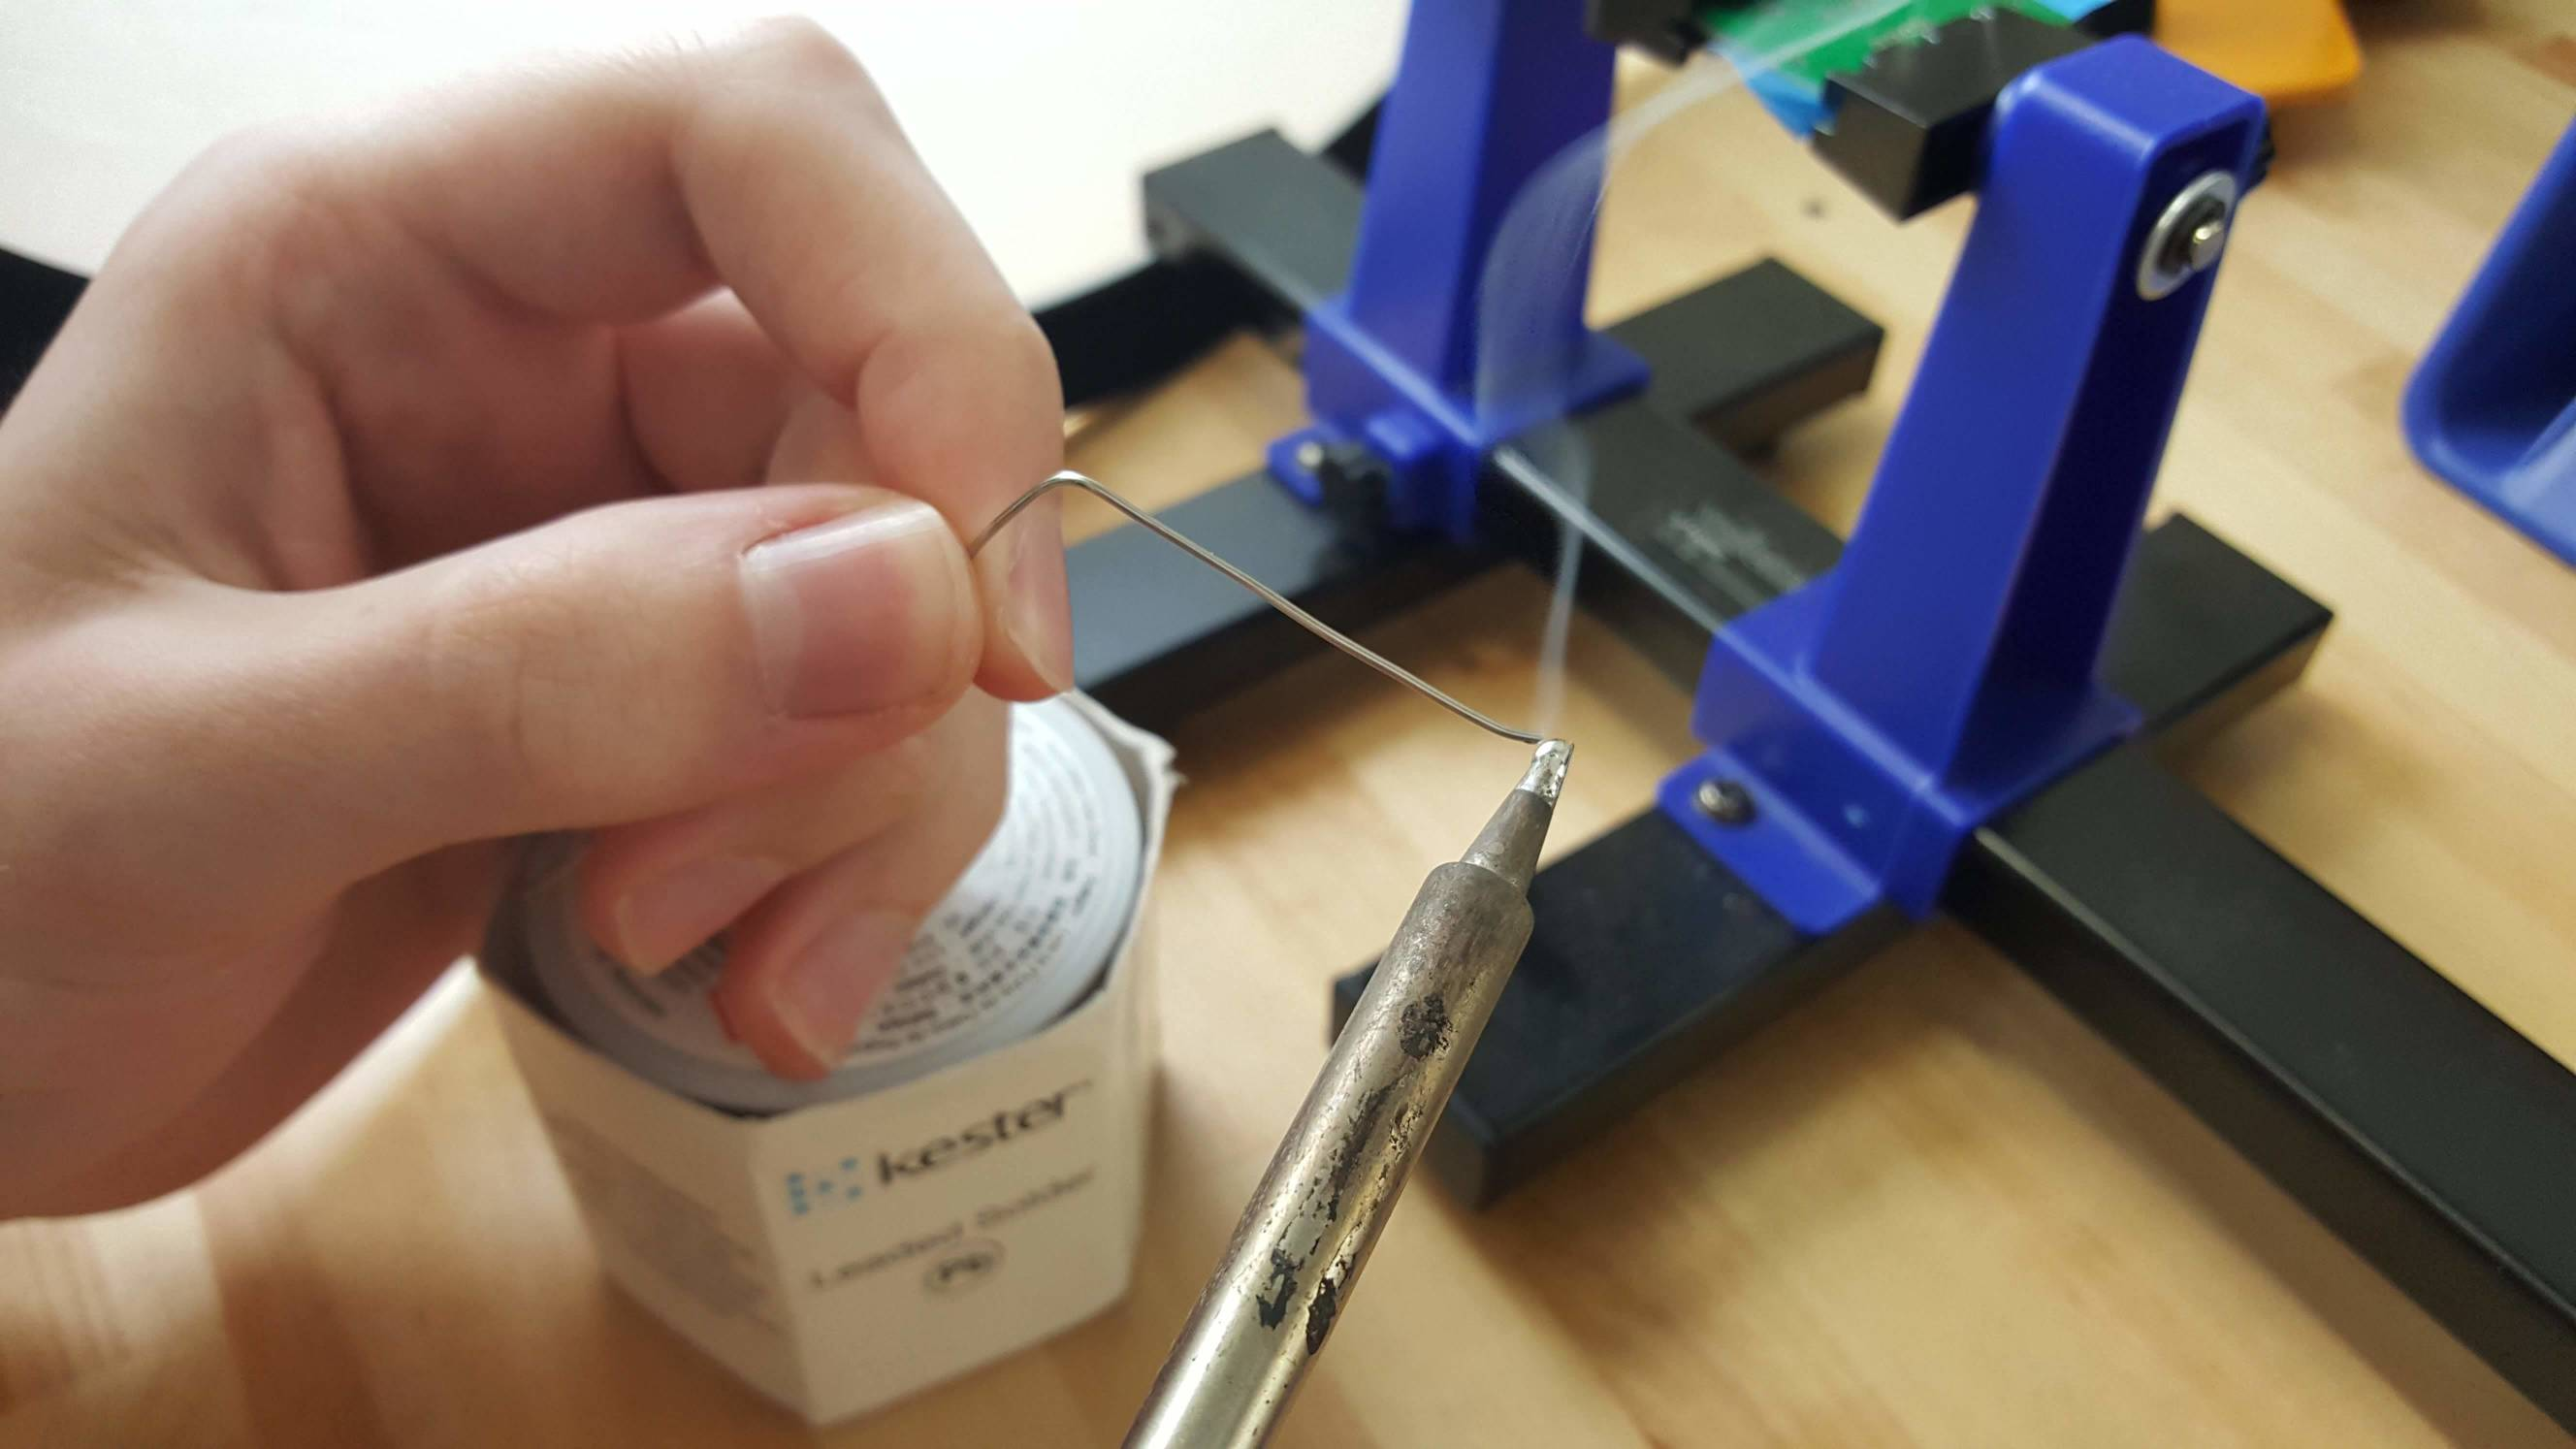
\includegraphics[width=0.75\textwidth]{img/0009.jpg}
\end{figure}

      
\begin{figure}[H]
\caption{ Cleaning the Iron Tip with the brass wool }
\label{fig:img/0011.jpg}
\centering
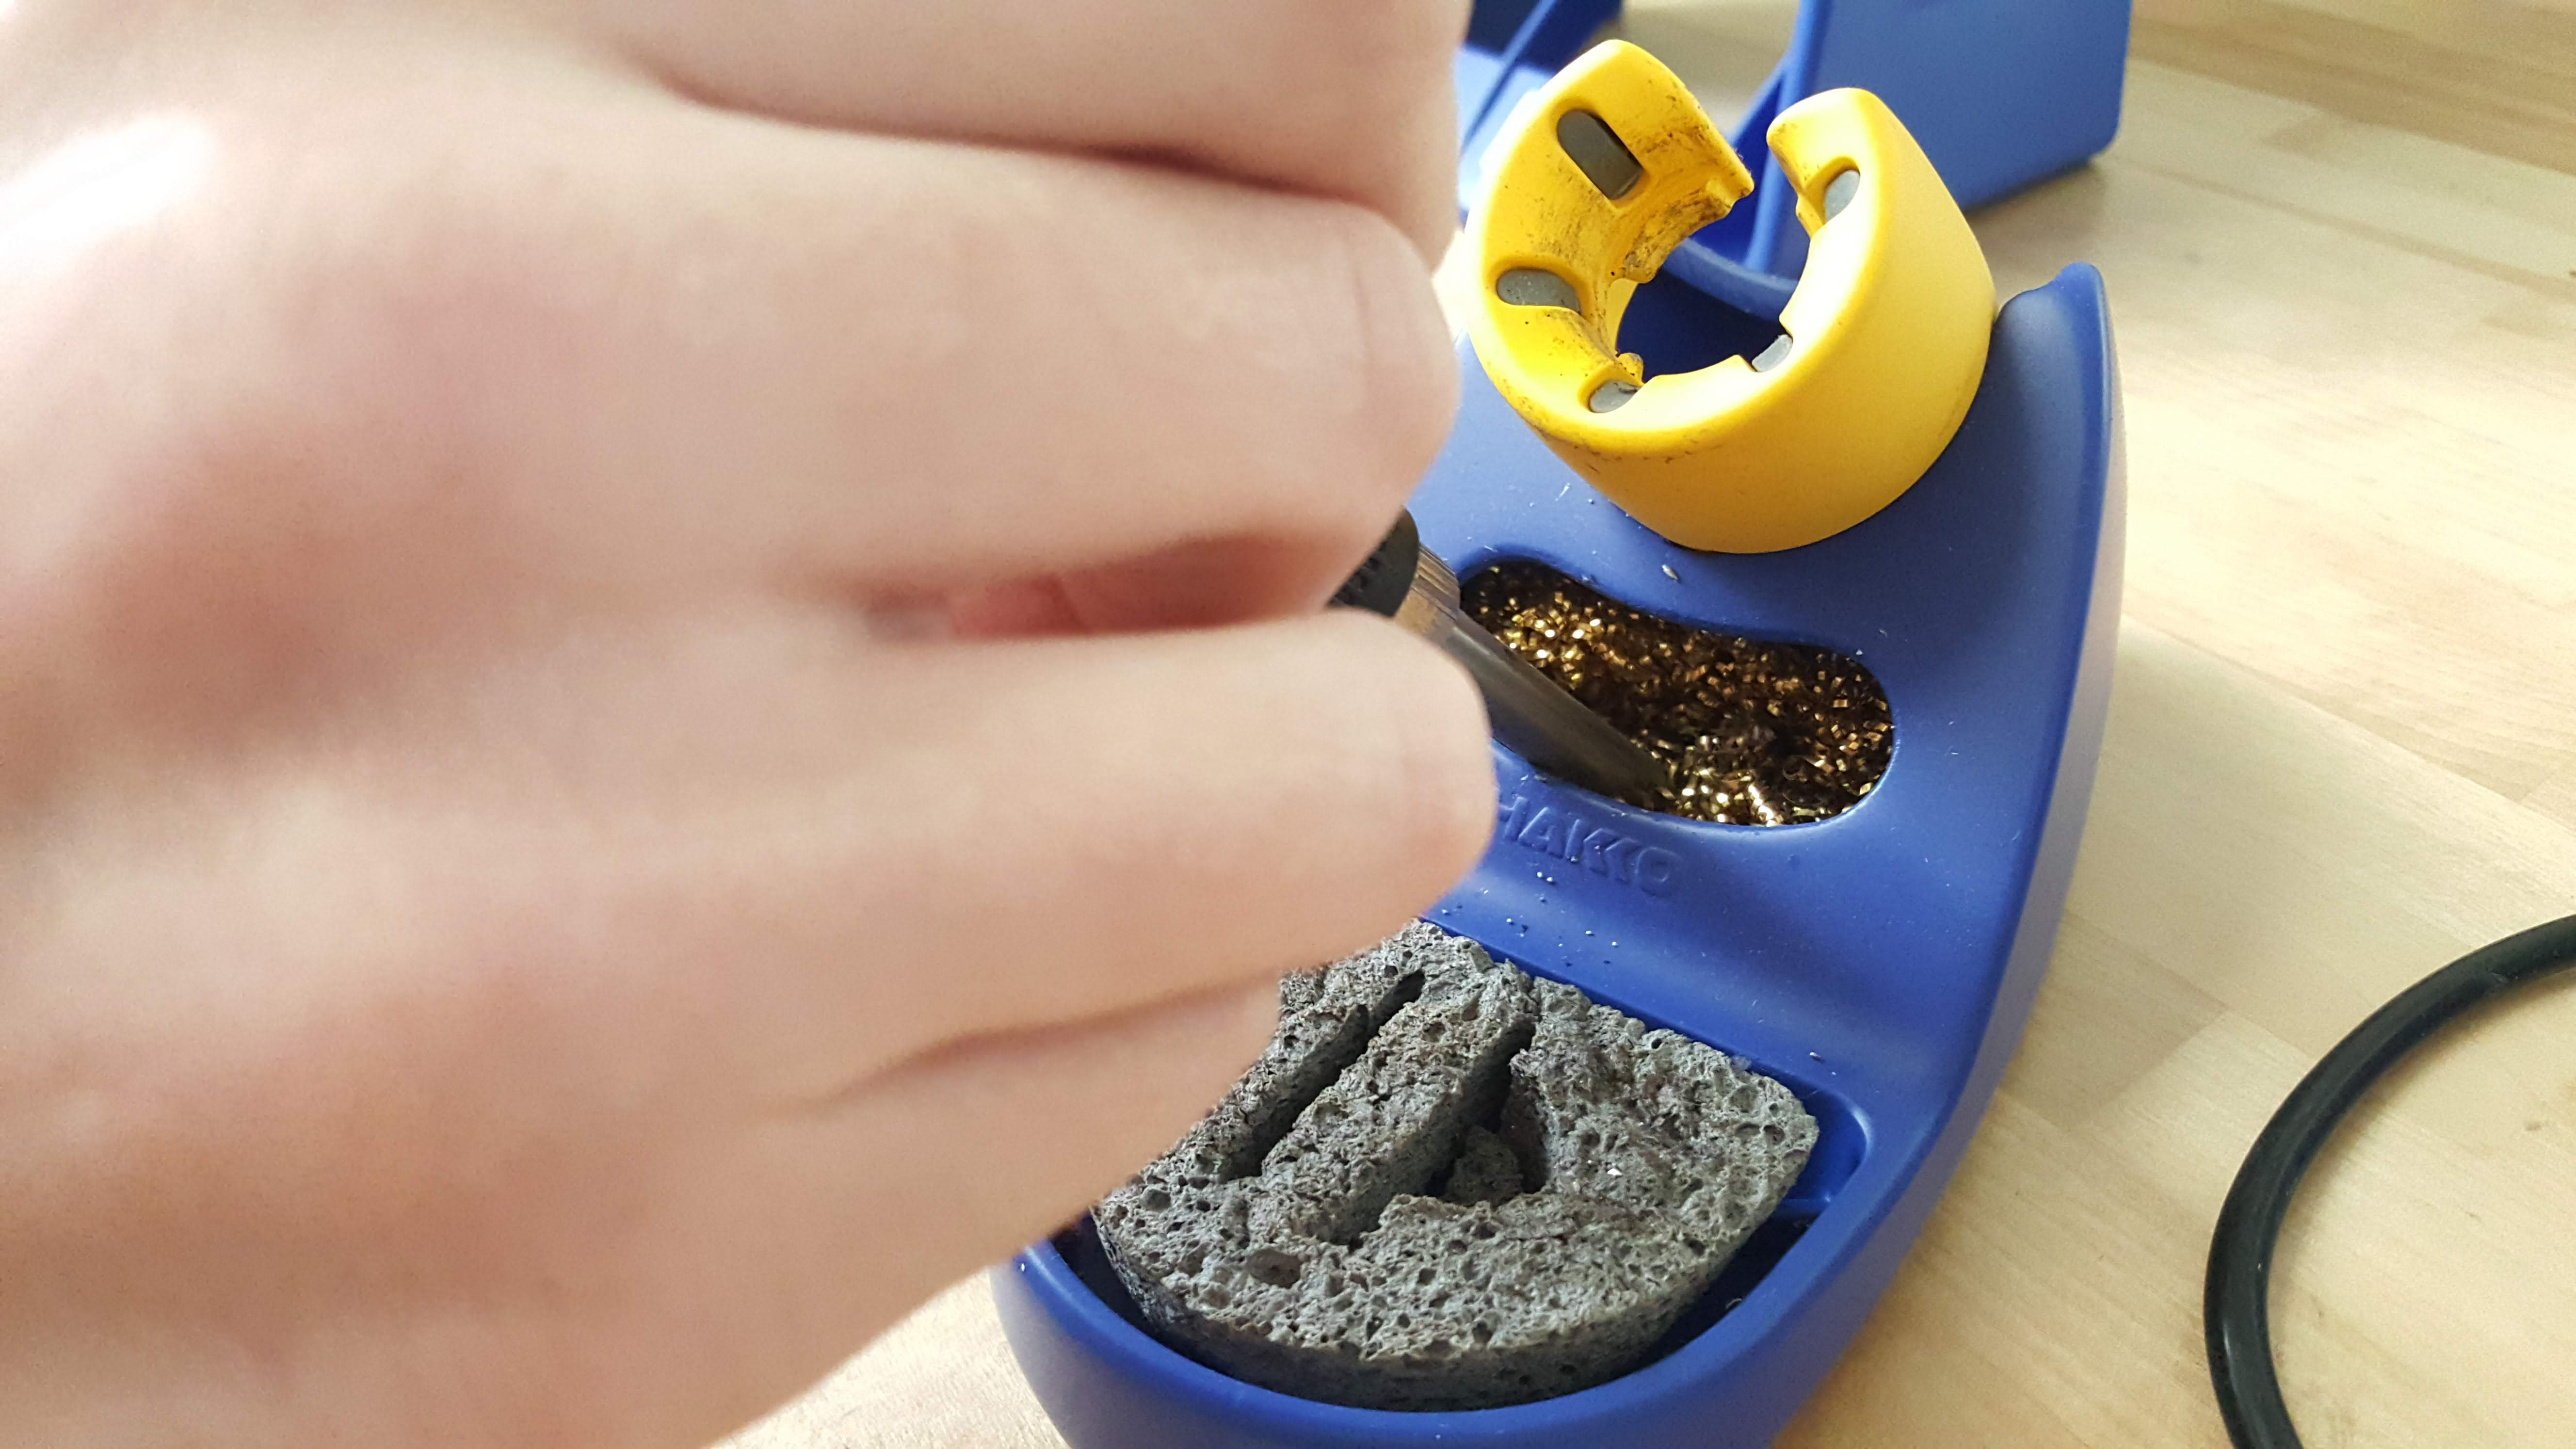
\includegraphics[width=0.75\textwidth]{img/0011.jpg}
\end{figure}

      \item 
      The iron is touched to the resistor's \textit{pad} (the metal ring around the hole).
      The solder is then pressed against the pad until it flows onto the joint. Once this happens remove the iron
      and allow it to cool before handling the part. Ideally, you should use just enough solder to make an
      even cone shape around the wire. The solder should also look shiny, if this is not the case,
      it is called a cold solder joint. These tend to be more brittle and can be fixed by reheating the joint.
      However, avoid heating anything for too long. The parts on the board, as well as
      the circuit board can be damaged by excess heat.

      \textbf{Note:} Applying solder directly to the iron isn't an effective way to solder.
       Liquid solder gravitates to hotter areas and it will accumulate where the temperature
       is at a local maximum. Meaning that the solder wont make it to the pad. Instead apply heat to where you
      want the solder to end up.
      
\begin{figure}[H]
\caption{ The Desired Wire }
\label{fig:img/0014.jpg}
\centering
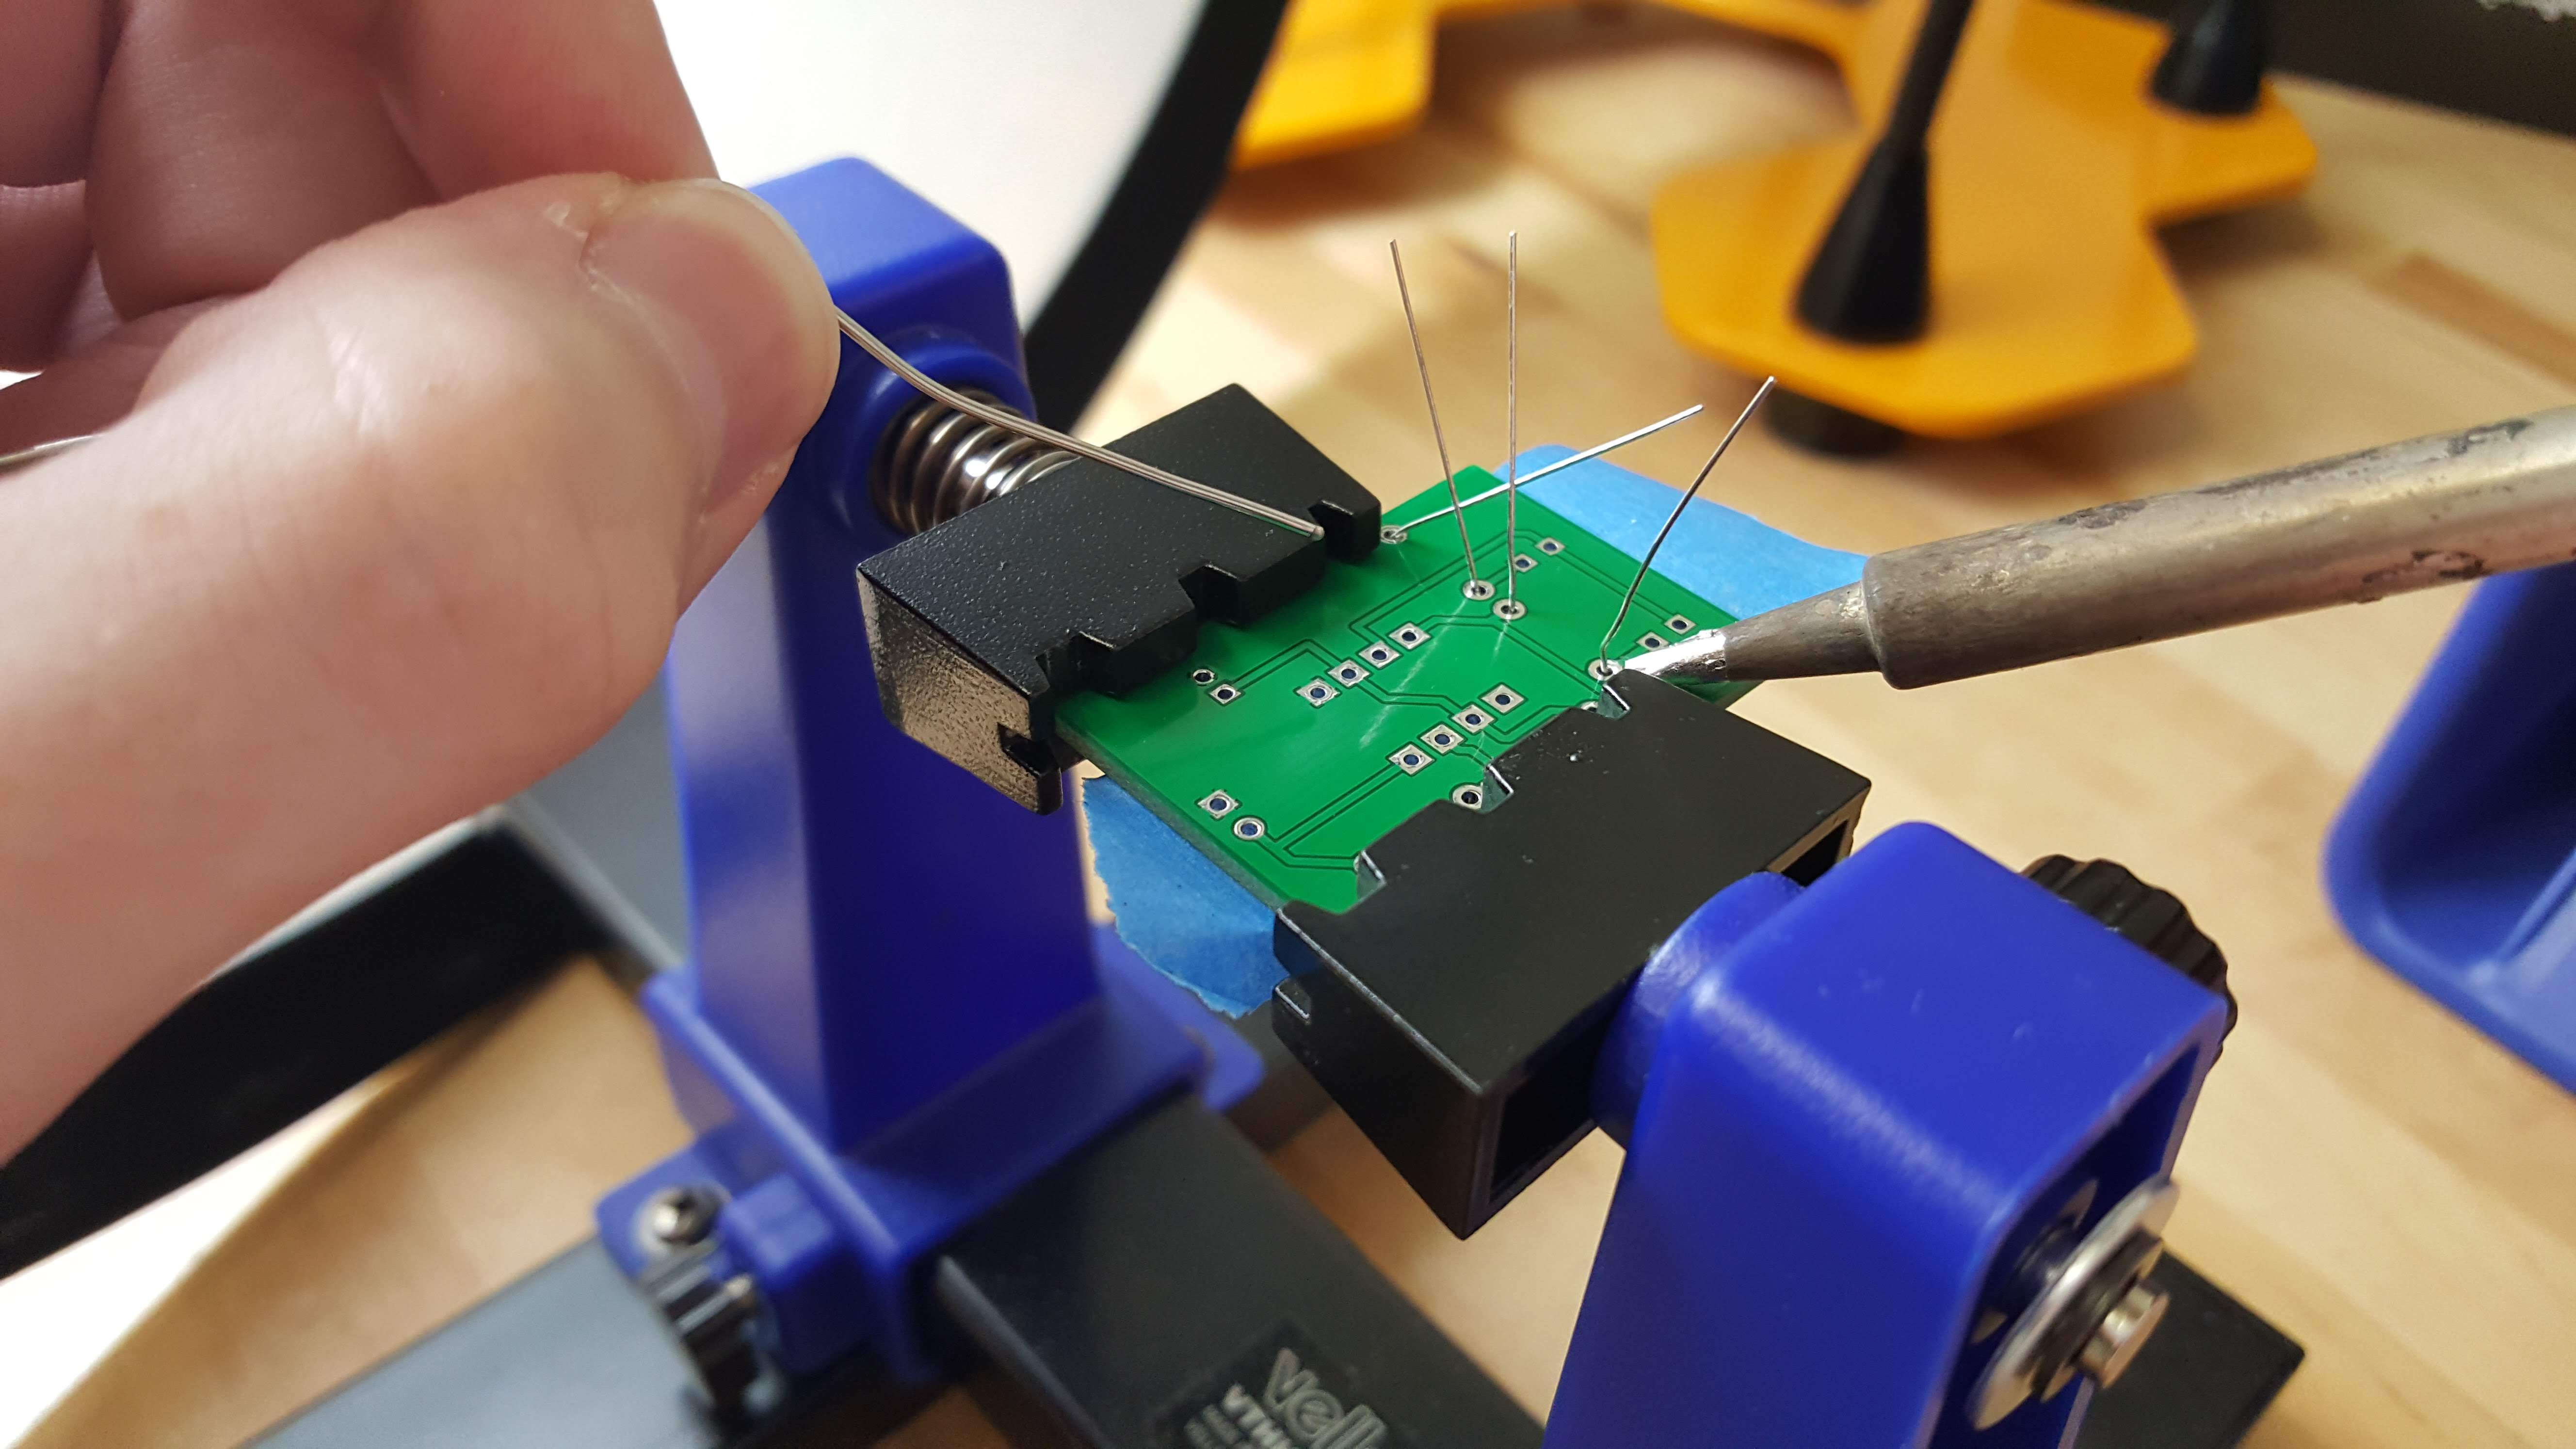
\includegraphics[width=0.75\textwidth]{img/0014.jpg}
\end{figure}

      
\begin{figure}[H]
\caption{ Applying Heat and Solder }
\label{fig:img/0015.jpg}
\centering
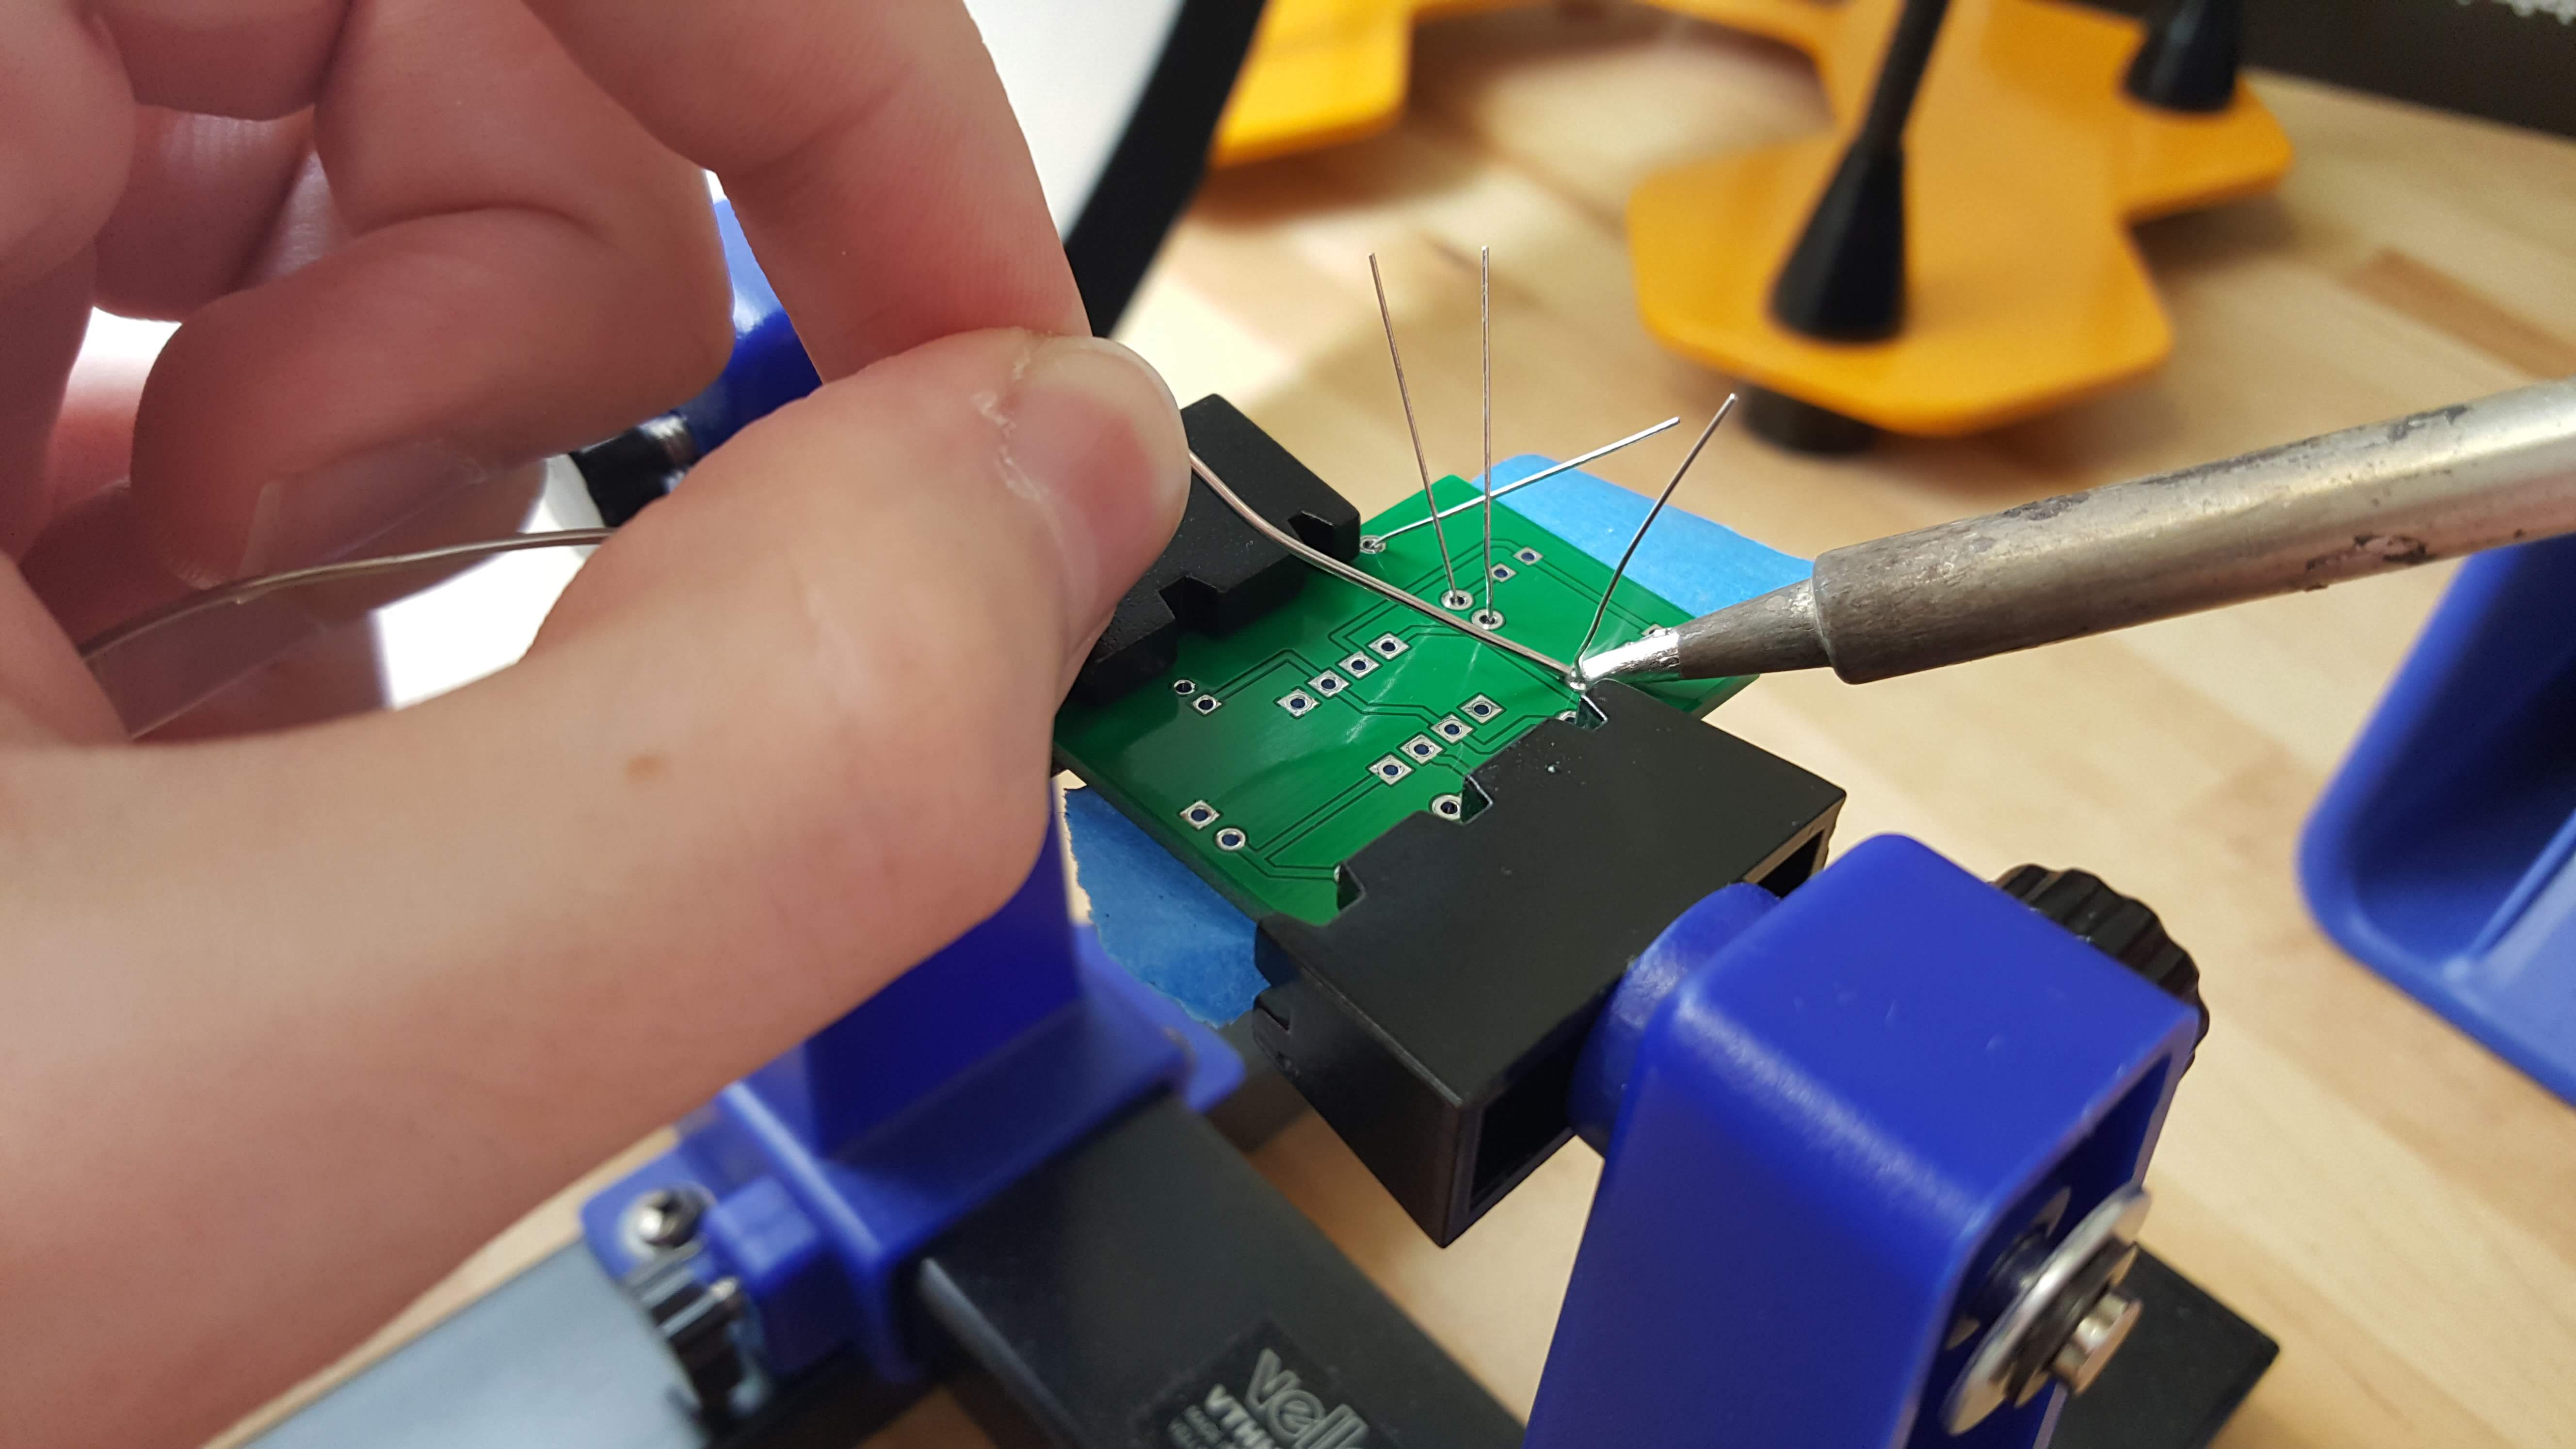
\includegraphics[width=0.75\textwidth]{img/0015.jpg}
\end{figure}

      
\begin{figure}[H]
\caption{ Close Up }
\label{fig:img/0015b.jpg}
\centering
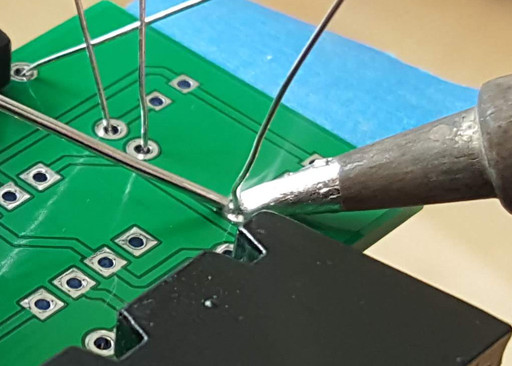
\includegraphics[width=0.75\textwidth]{img/0015b.jpg}
\end{figure}

      \item 
      Next the leads need to be snipped to reduce their length. They can be snipped right where the cone of solder converges to the lead. Be careful, when
      snipping these leads, they can go flying through the air. Safety glasses are advised throughout this process.
      
\begin{figure}[H]
\caption{ Snipping the Leads }
\label{fig:img/0018.jpg}
\centering
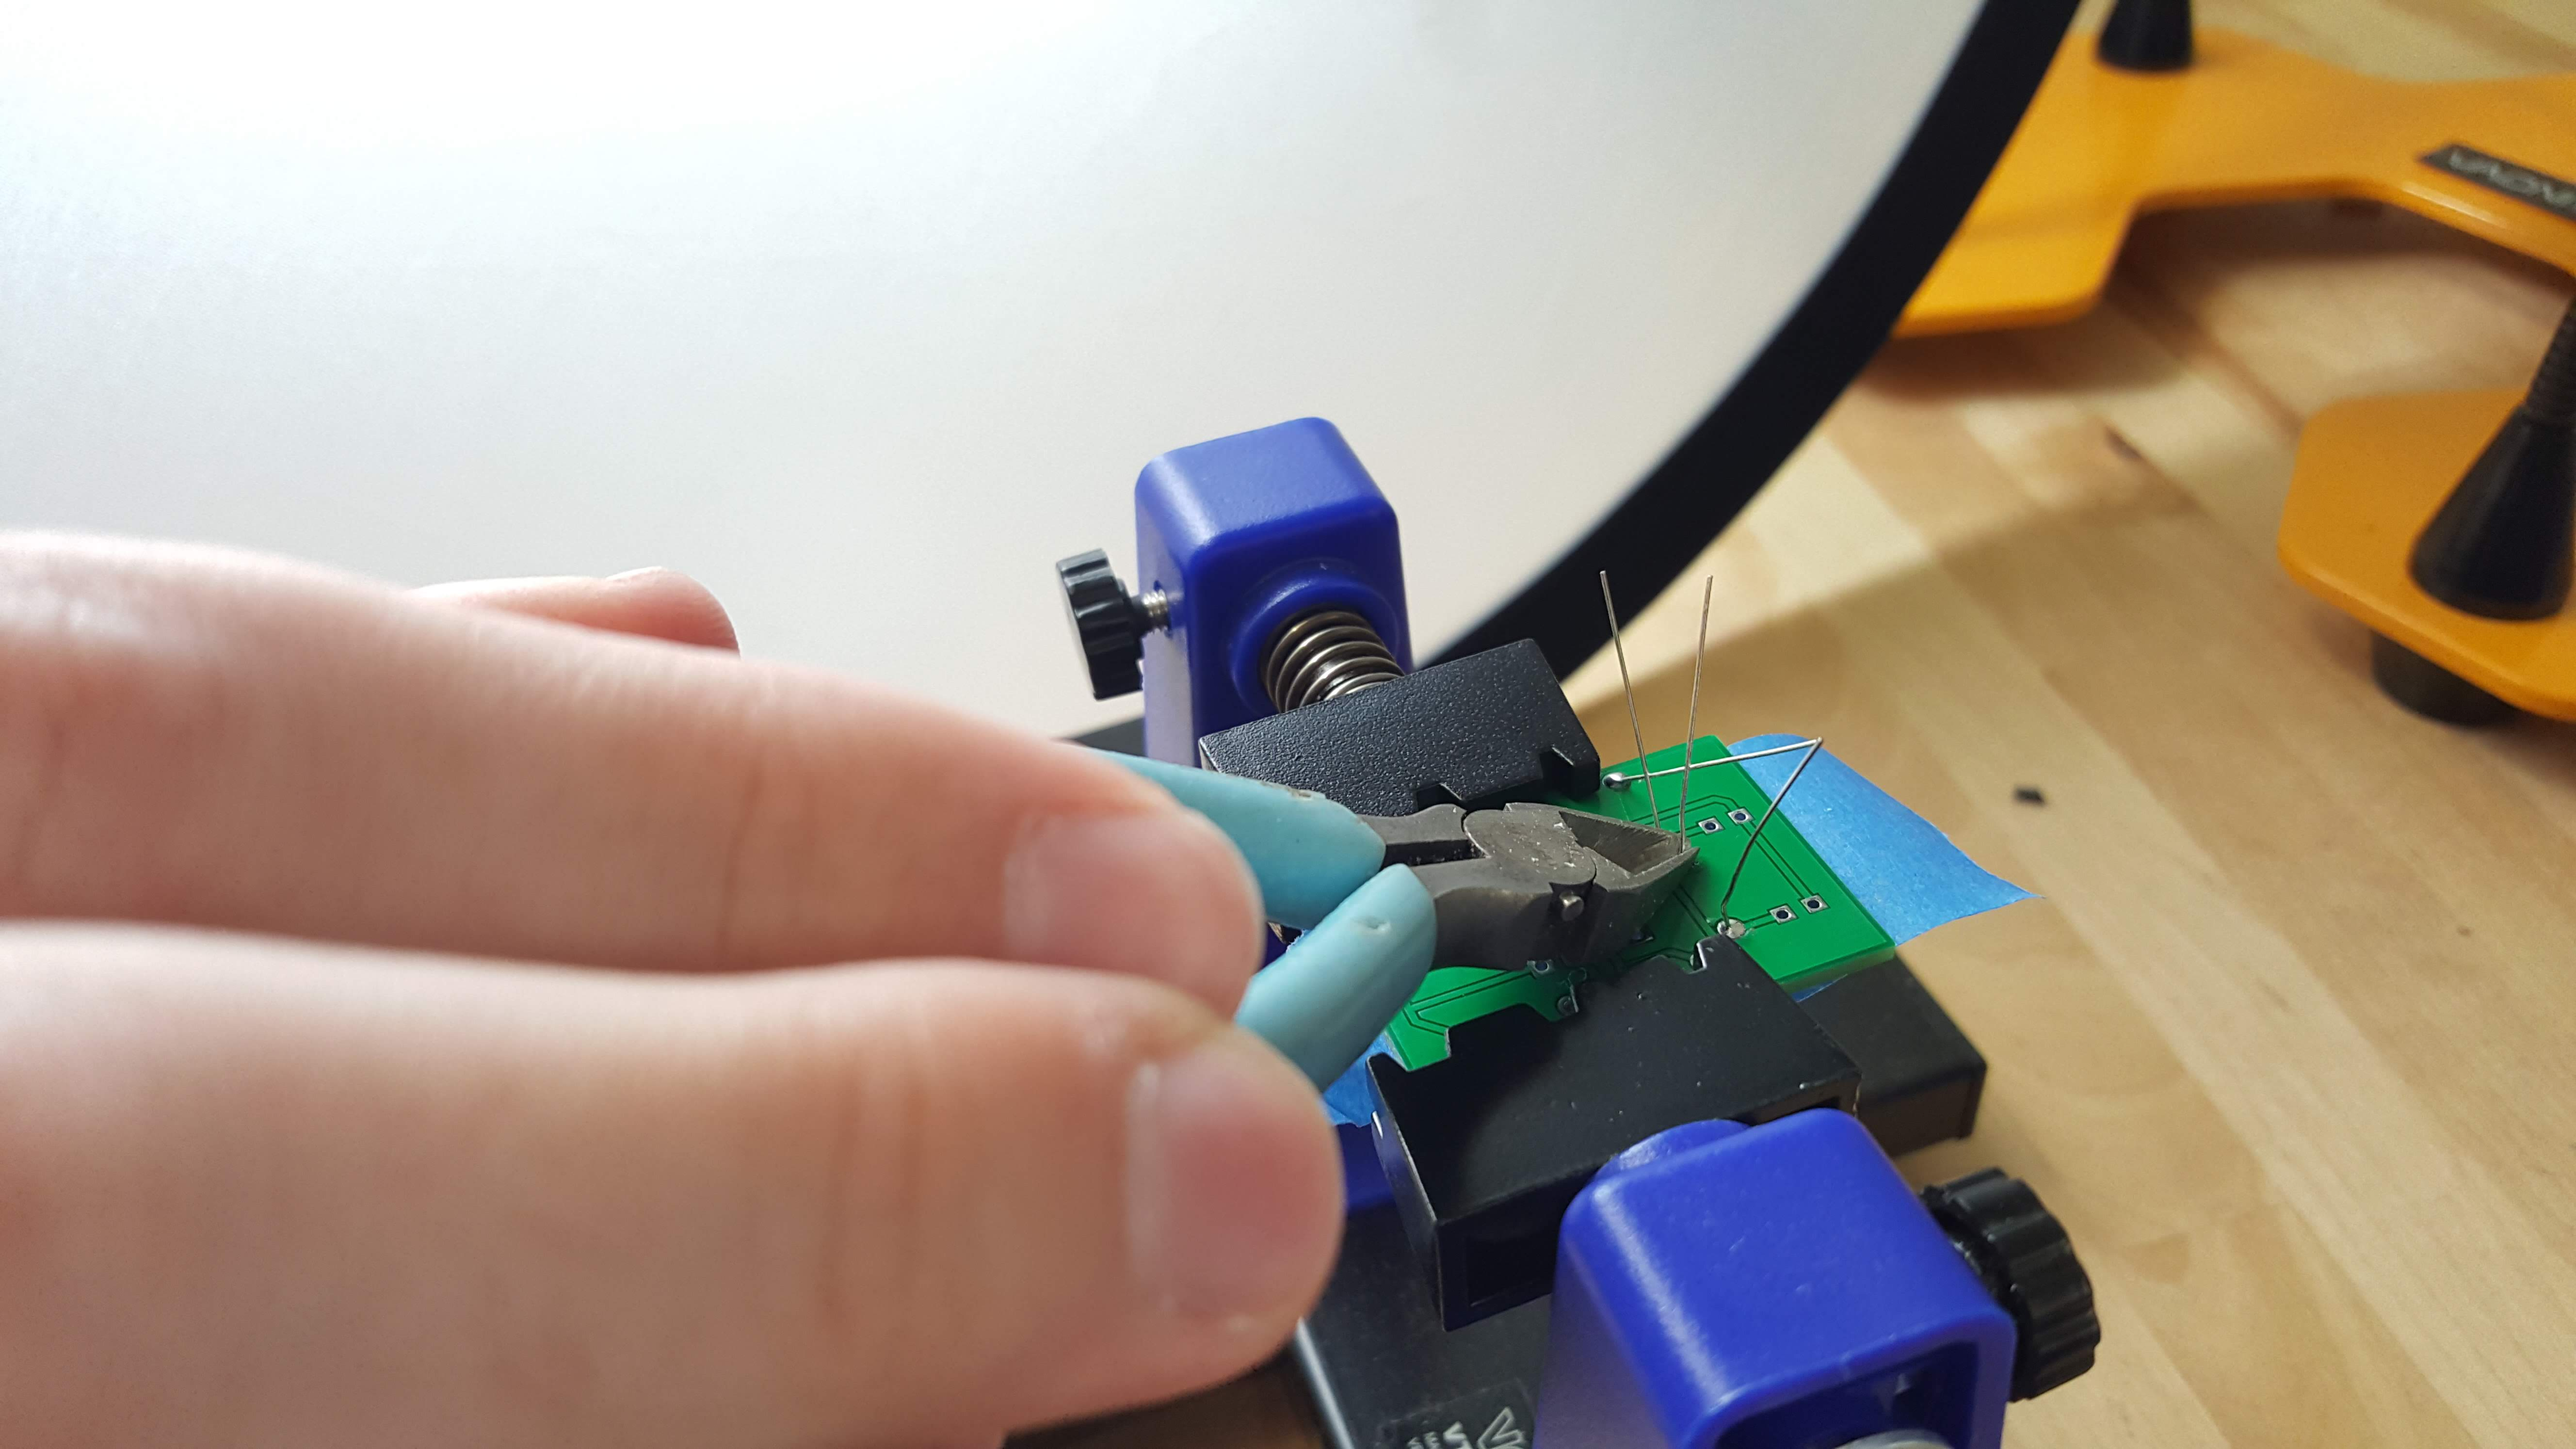
\includegraphics[width=0.75\textwidth]{img/0018.jpg}
\end{figure}

      \item   The next resistors to solder are R1 ($1k\Omega$), and R2($10k\Omega$). The same steps are repeated for these.
      
\begin{figure}[H]
\caption{ Inserting R1, and R2 }
\label{fig:img/0021.jpg}
\centering
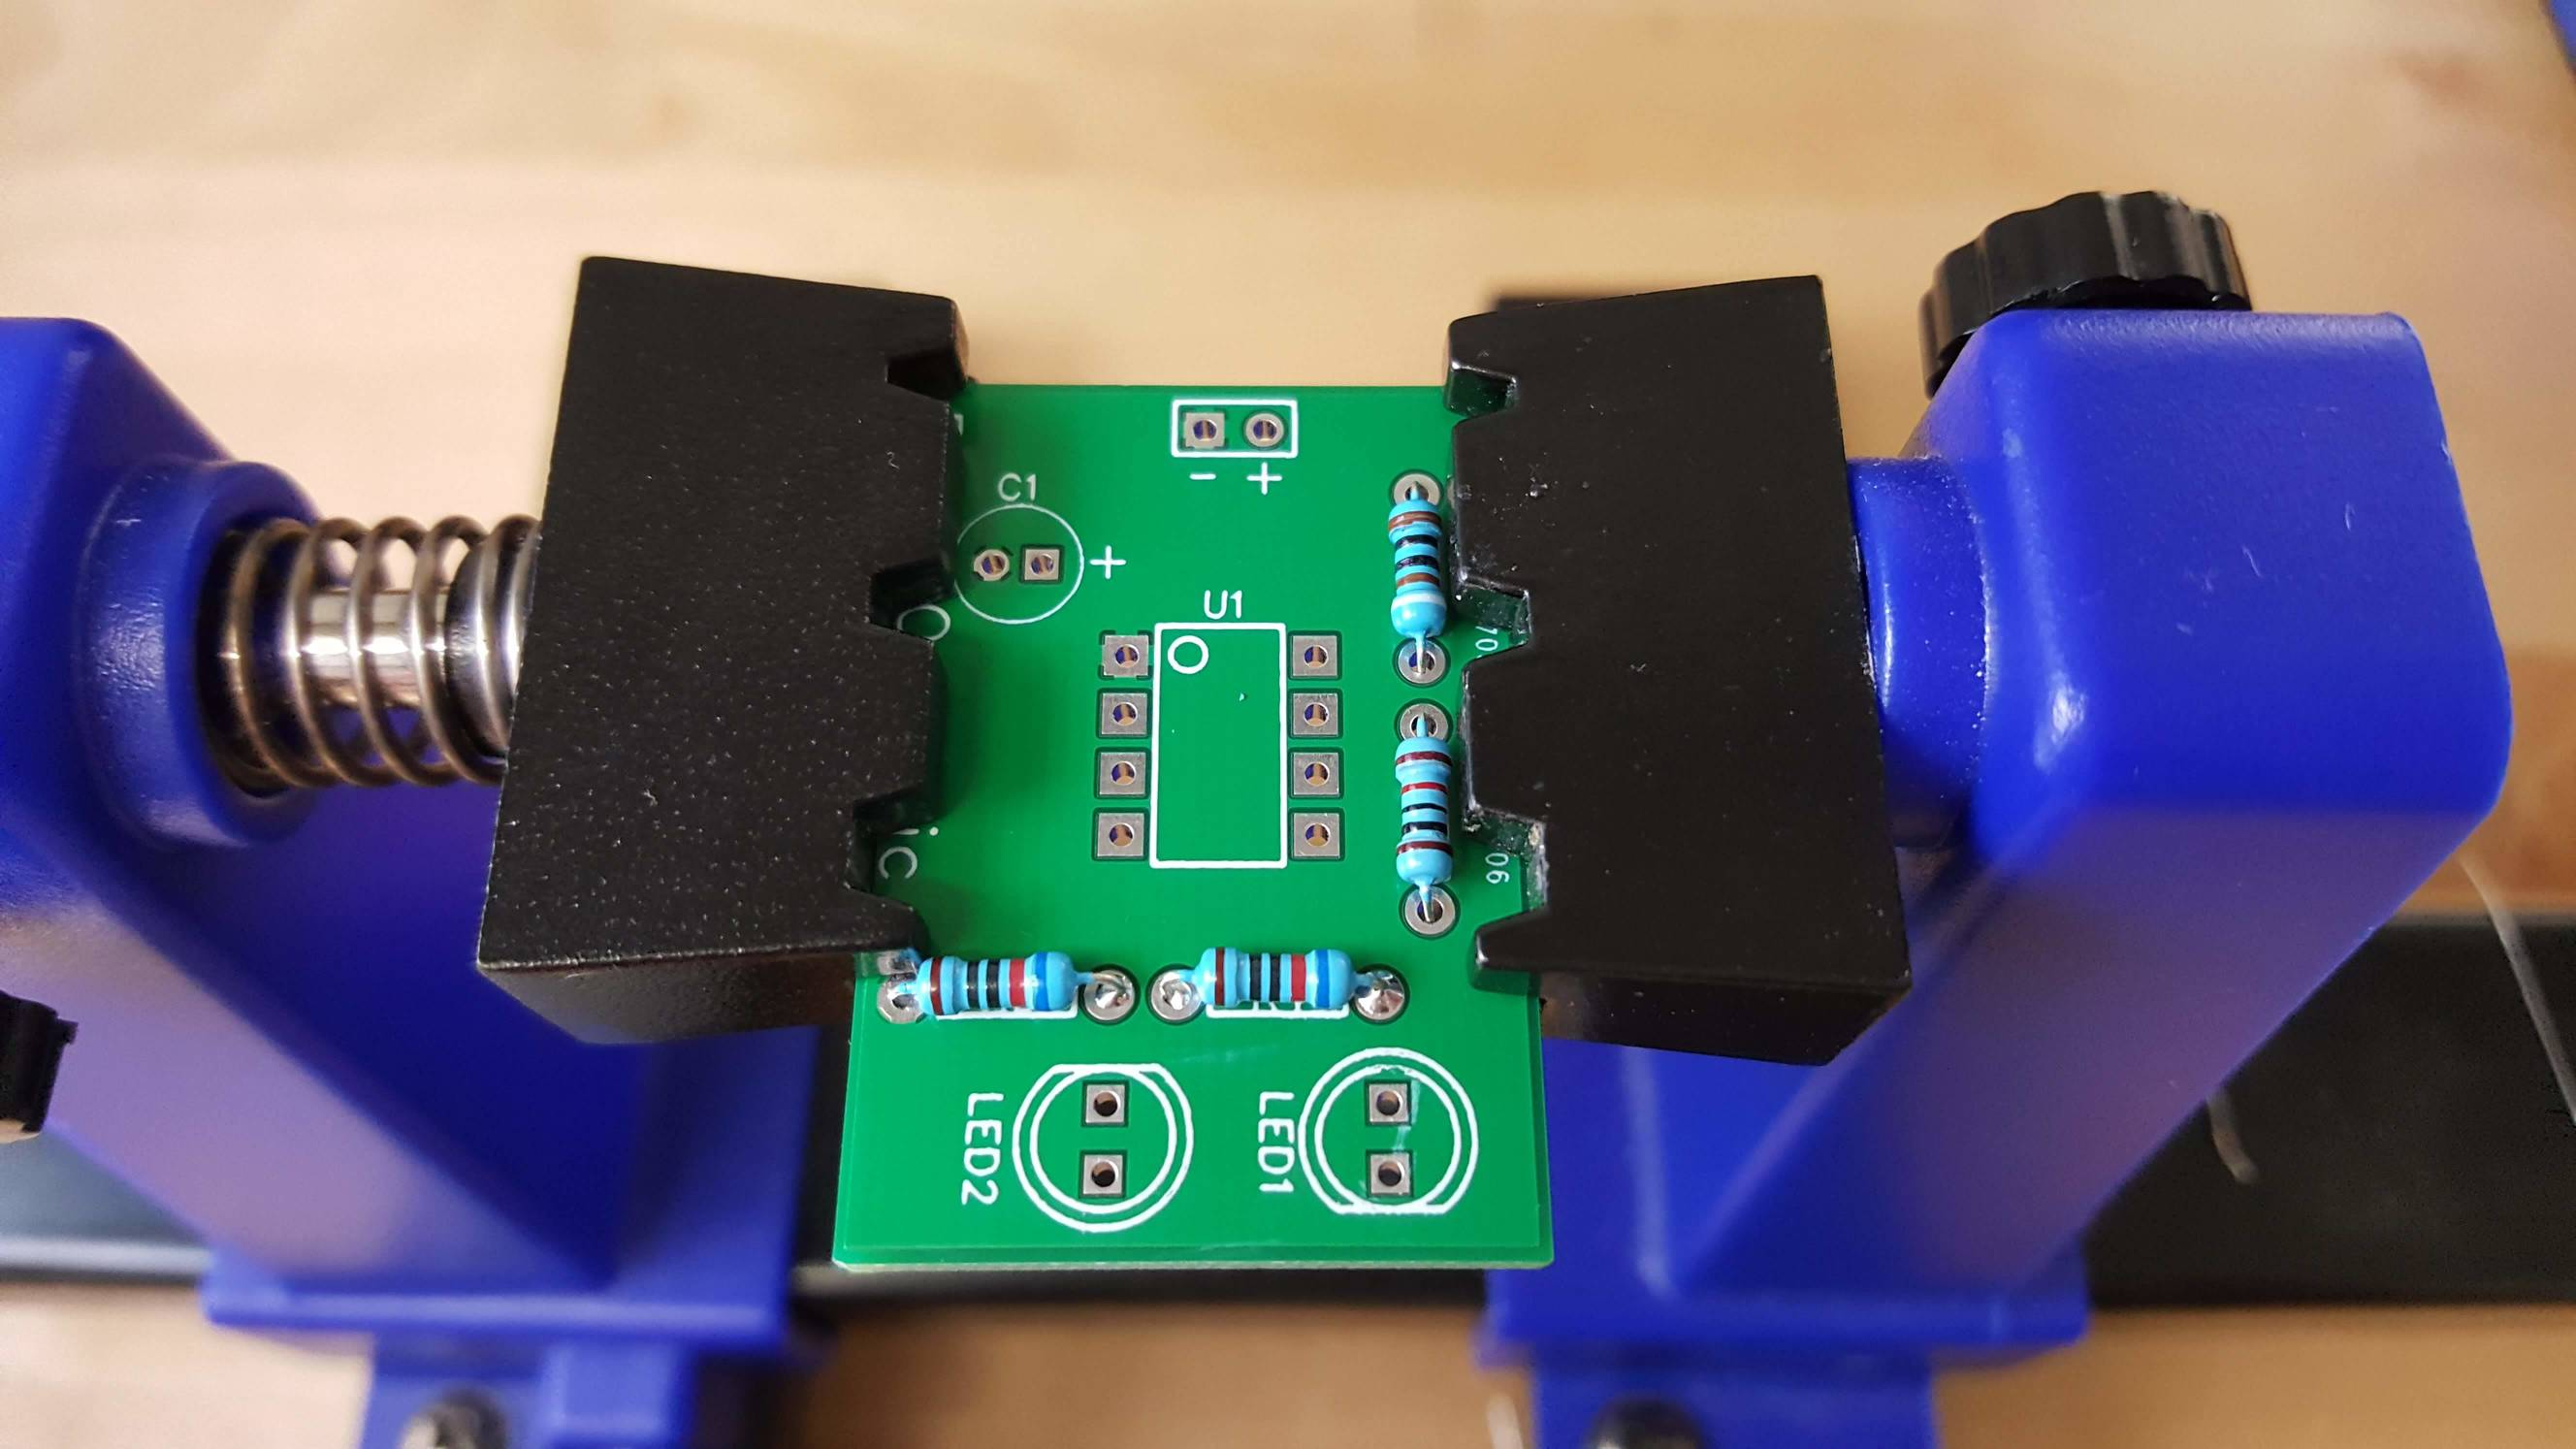
\includegraphics[width=0.75\textwidth]{img/0021.jpg}
\end{figure}

      
\begin{figure}[H]
\caption{ Soldering R1, and R2 }
\label{fig:img/0022.jpg}
\centering
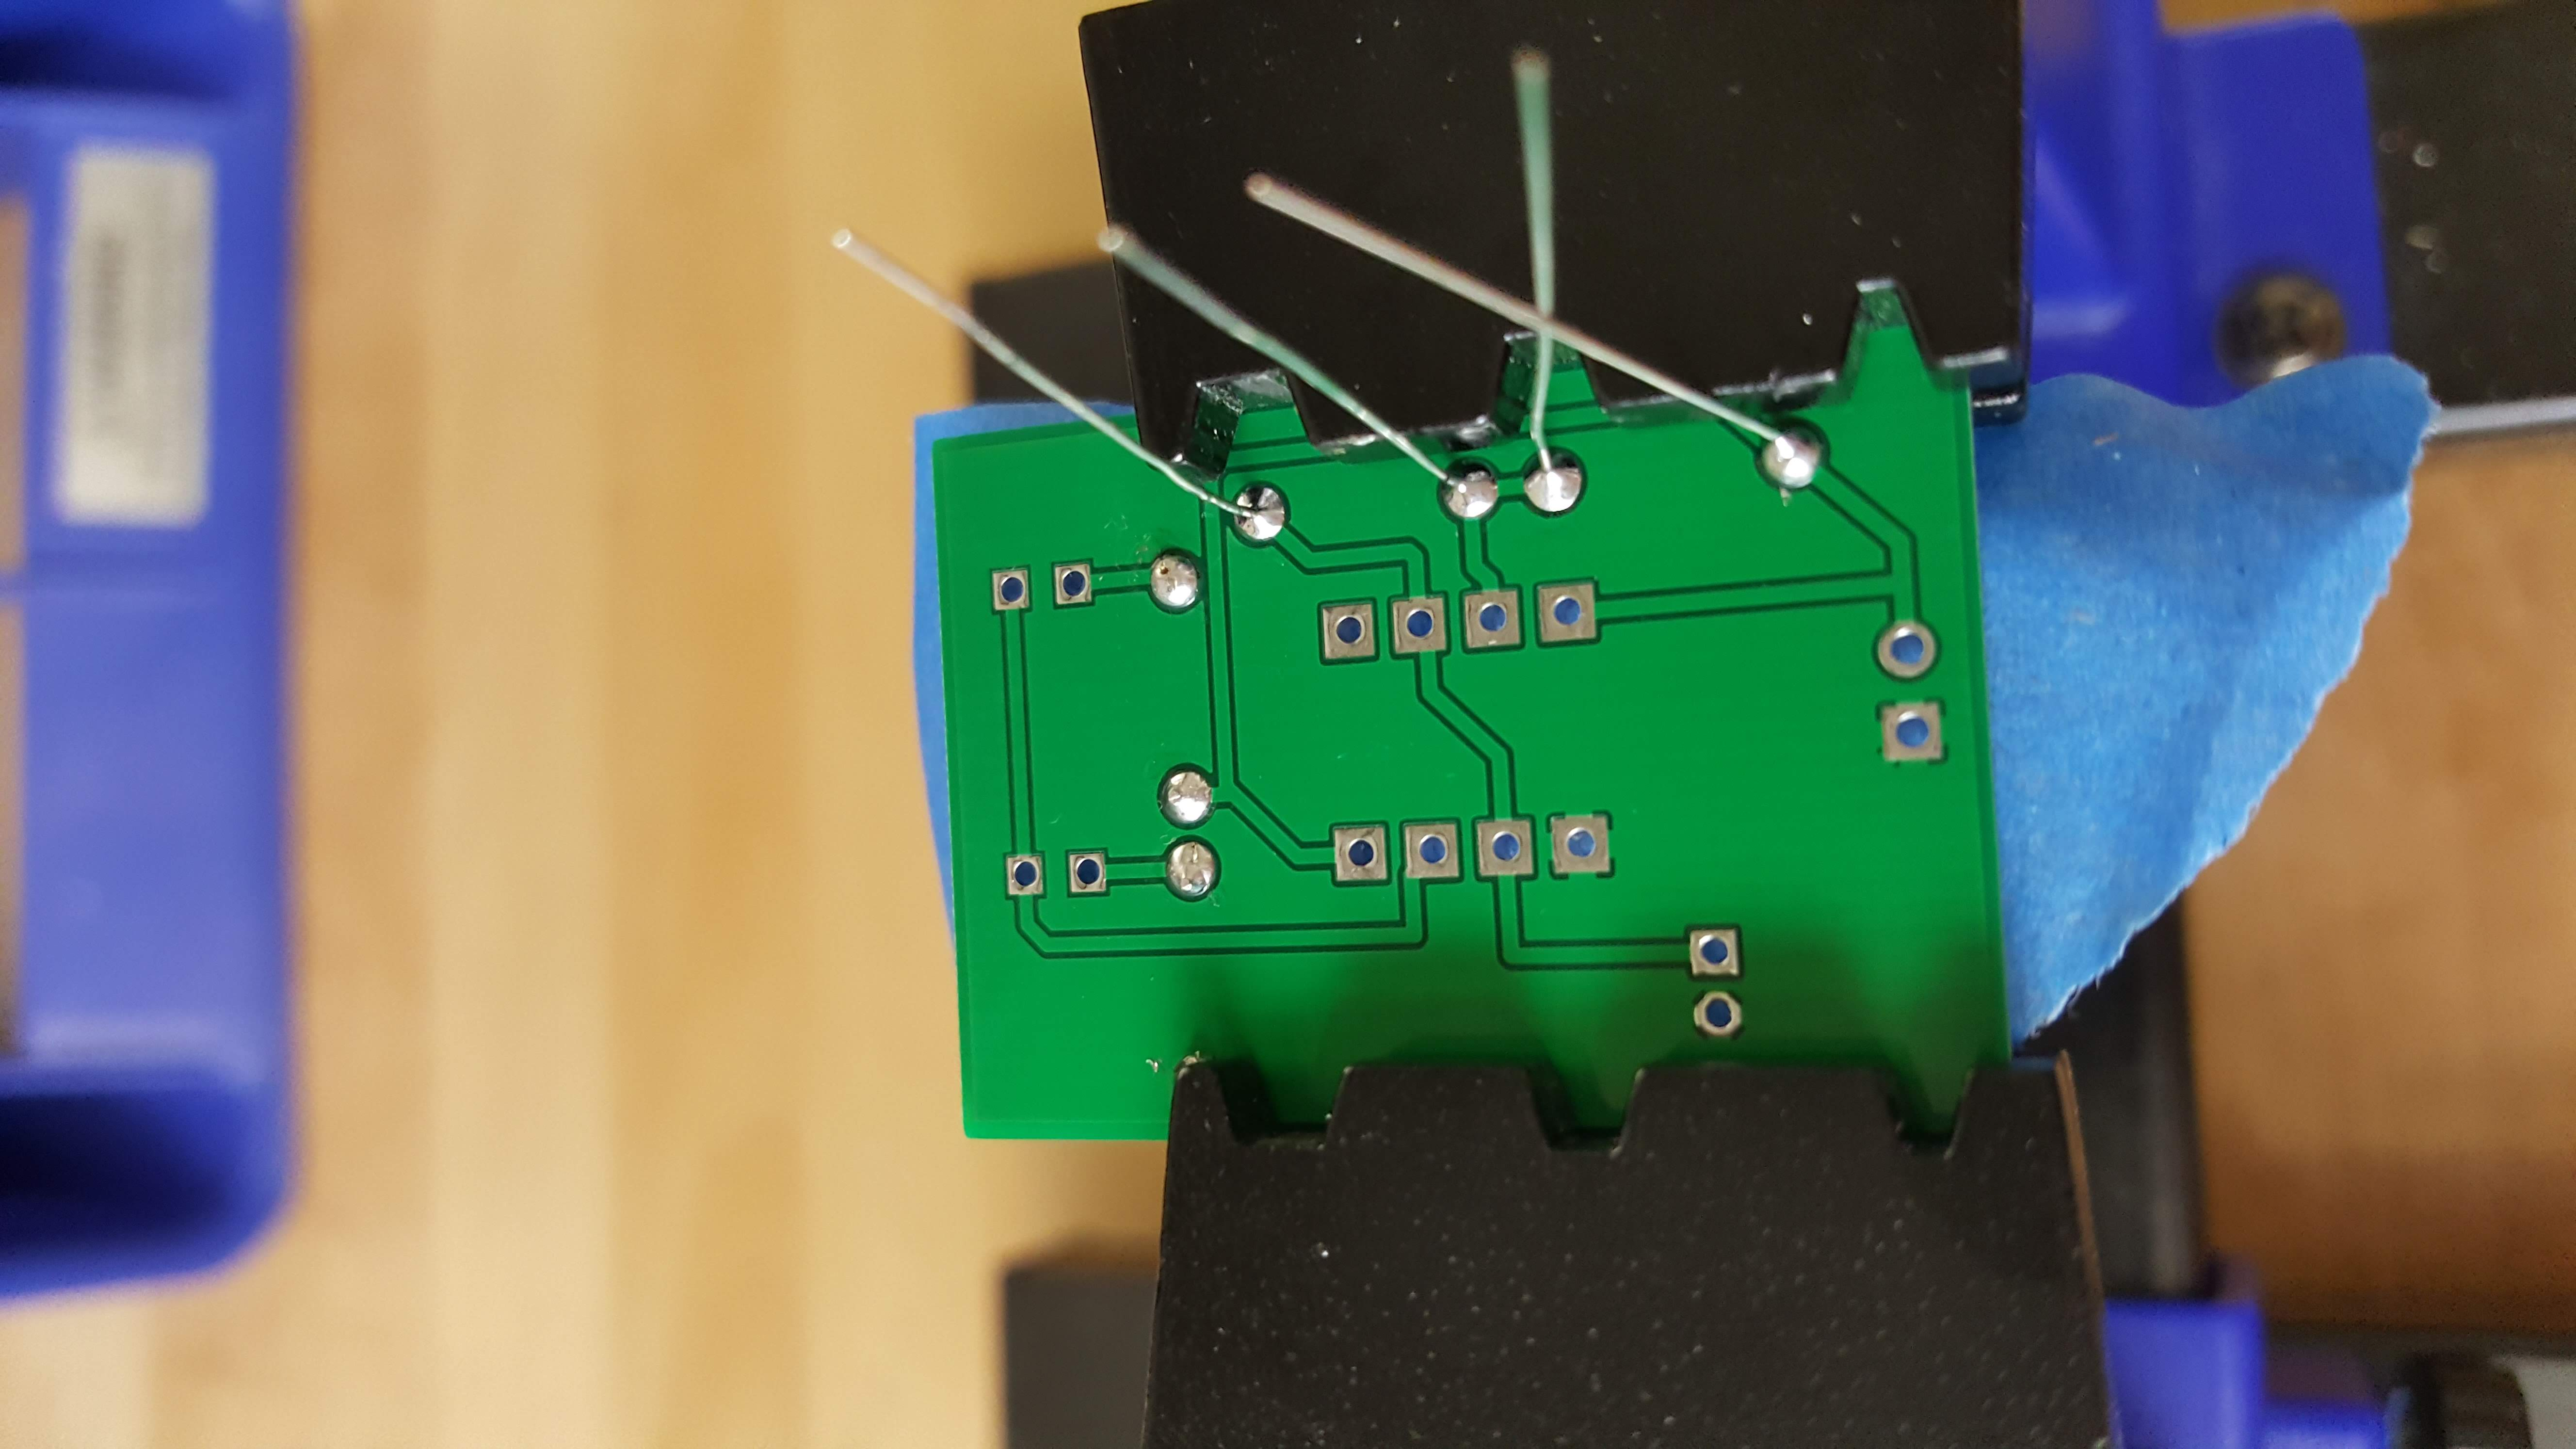
\includegraphics[width=0.75\textwidth]{img/0022.jpg}
\end{figure}

      
\begin{figure}[H]
\caption{ Snipping R1, and R2 }
\label{fig:img/0023.jpg}
\centering
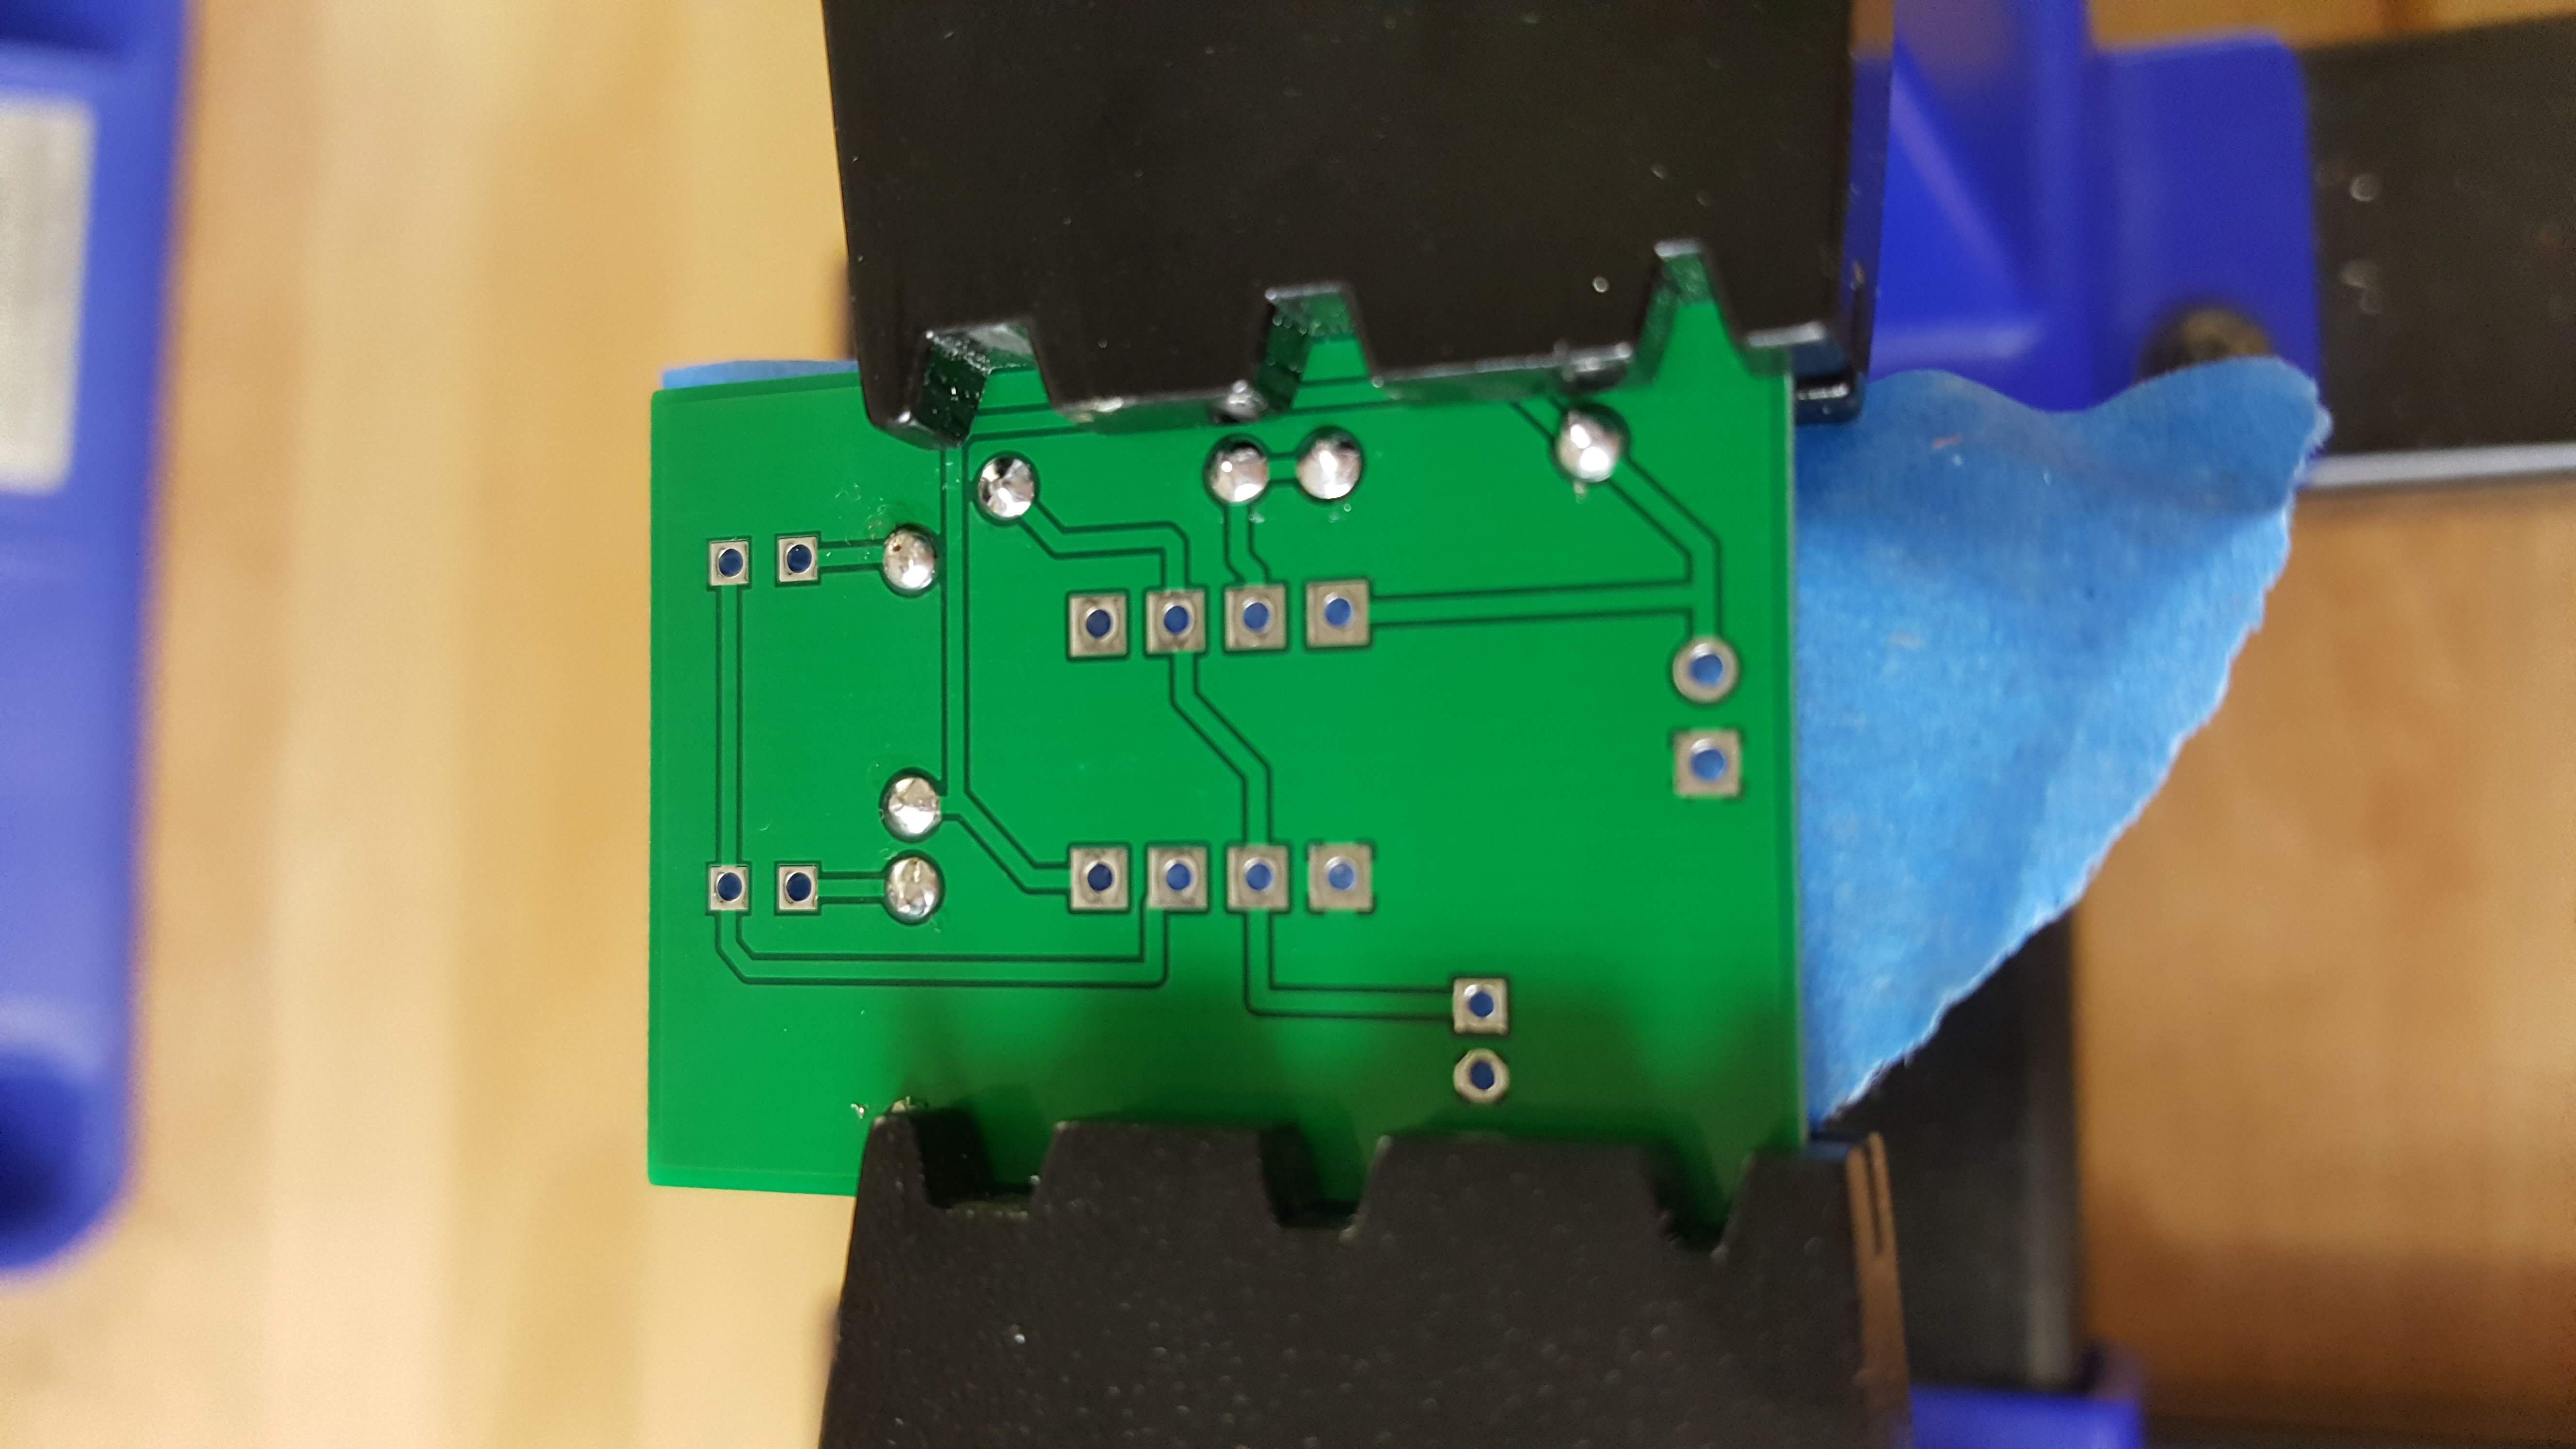
\includegraphics[width=0.75\textwidth]{img/0023.jpg}
\end{figure}

      \item 
      The integrated circuit can be soldered directly like in the photos, however, it is better practice to use IC sockets. IC sockets
      are beneficial, because ICs can easily be removed from the circuit if they are damaged. Additionally, the risk of overheating the IC
      while soldering is negated. The IC typically comes from the factory with leads that are not perfectly
      90 degrees. To make it fit, the leads need to be pushed together slightly. The IC and its socket will have a notch to indicate
      the top of the chip. When placing the IC, ensure that the notch corresponds with the dot on the circuit board.
      
\begin{figure}[H]
\caption{ Bending IC Leads }
\label{fig:img/0024.jpg}
\centering
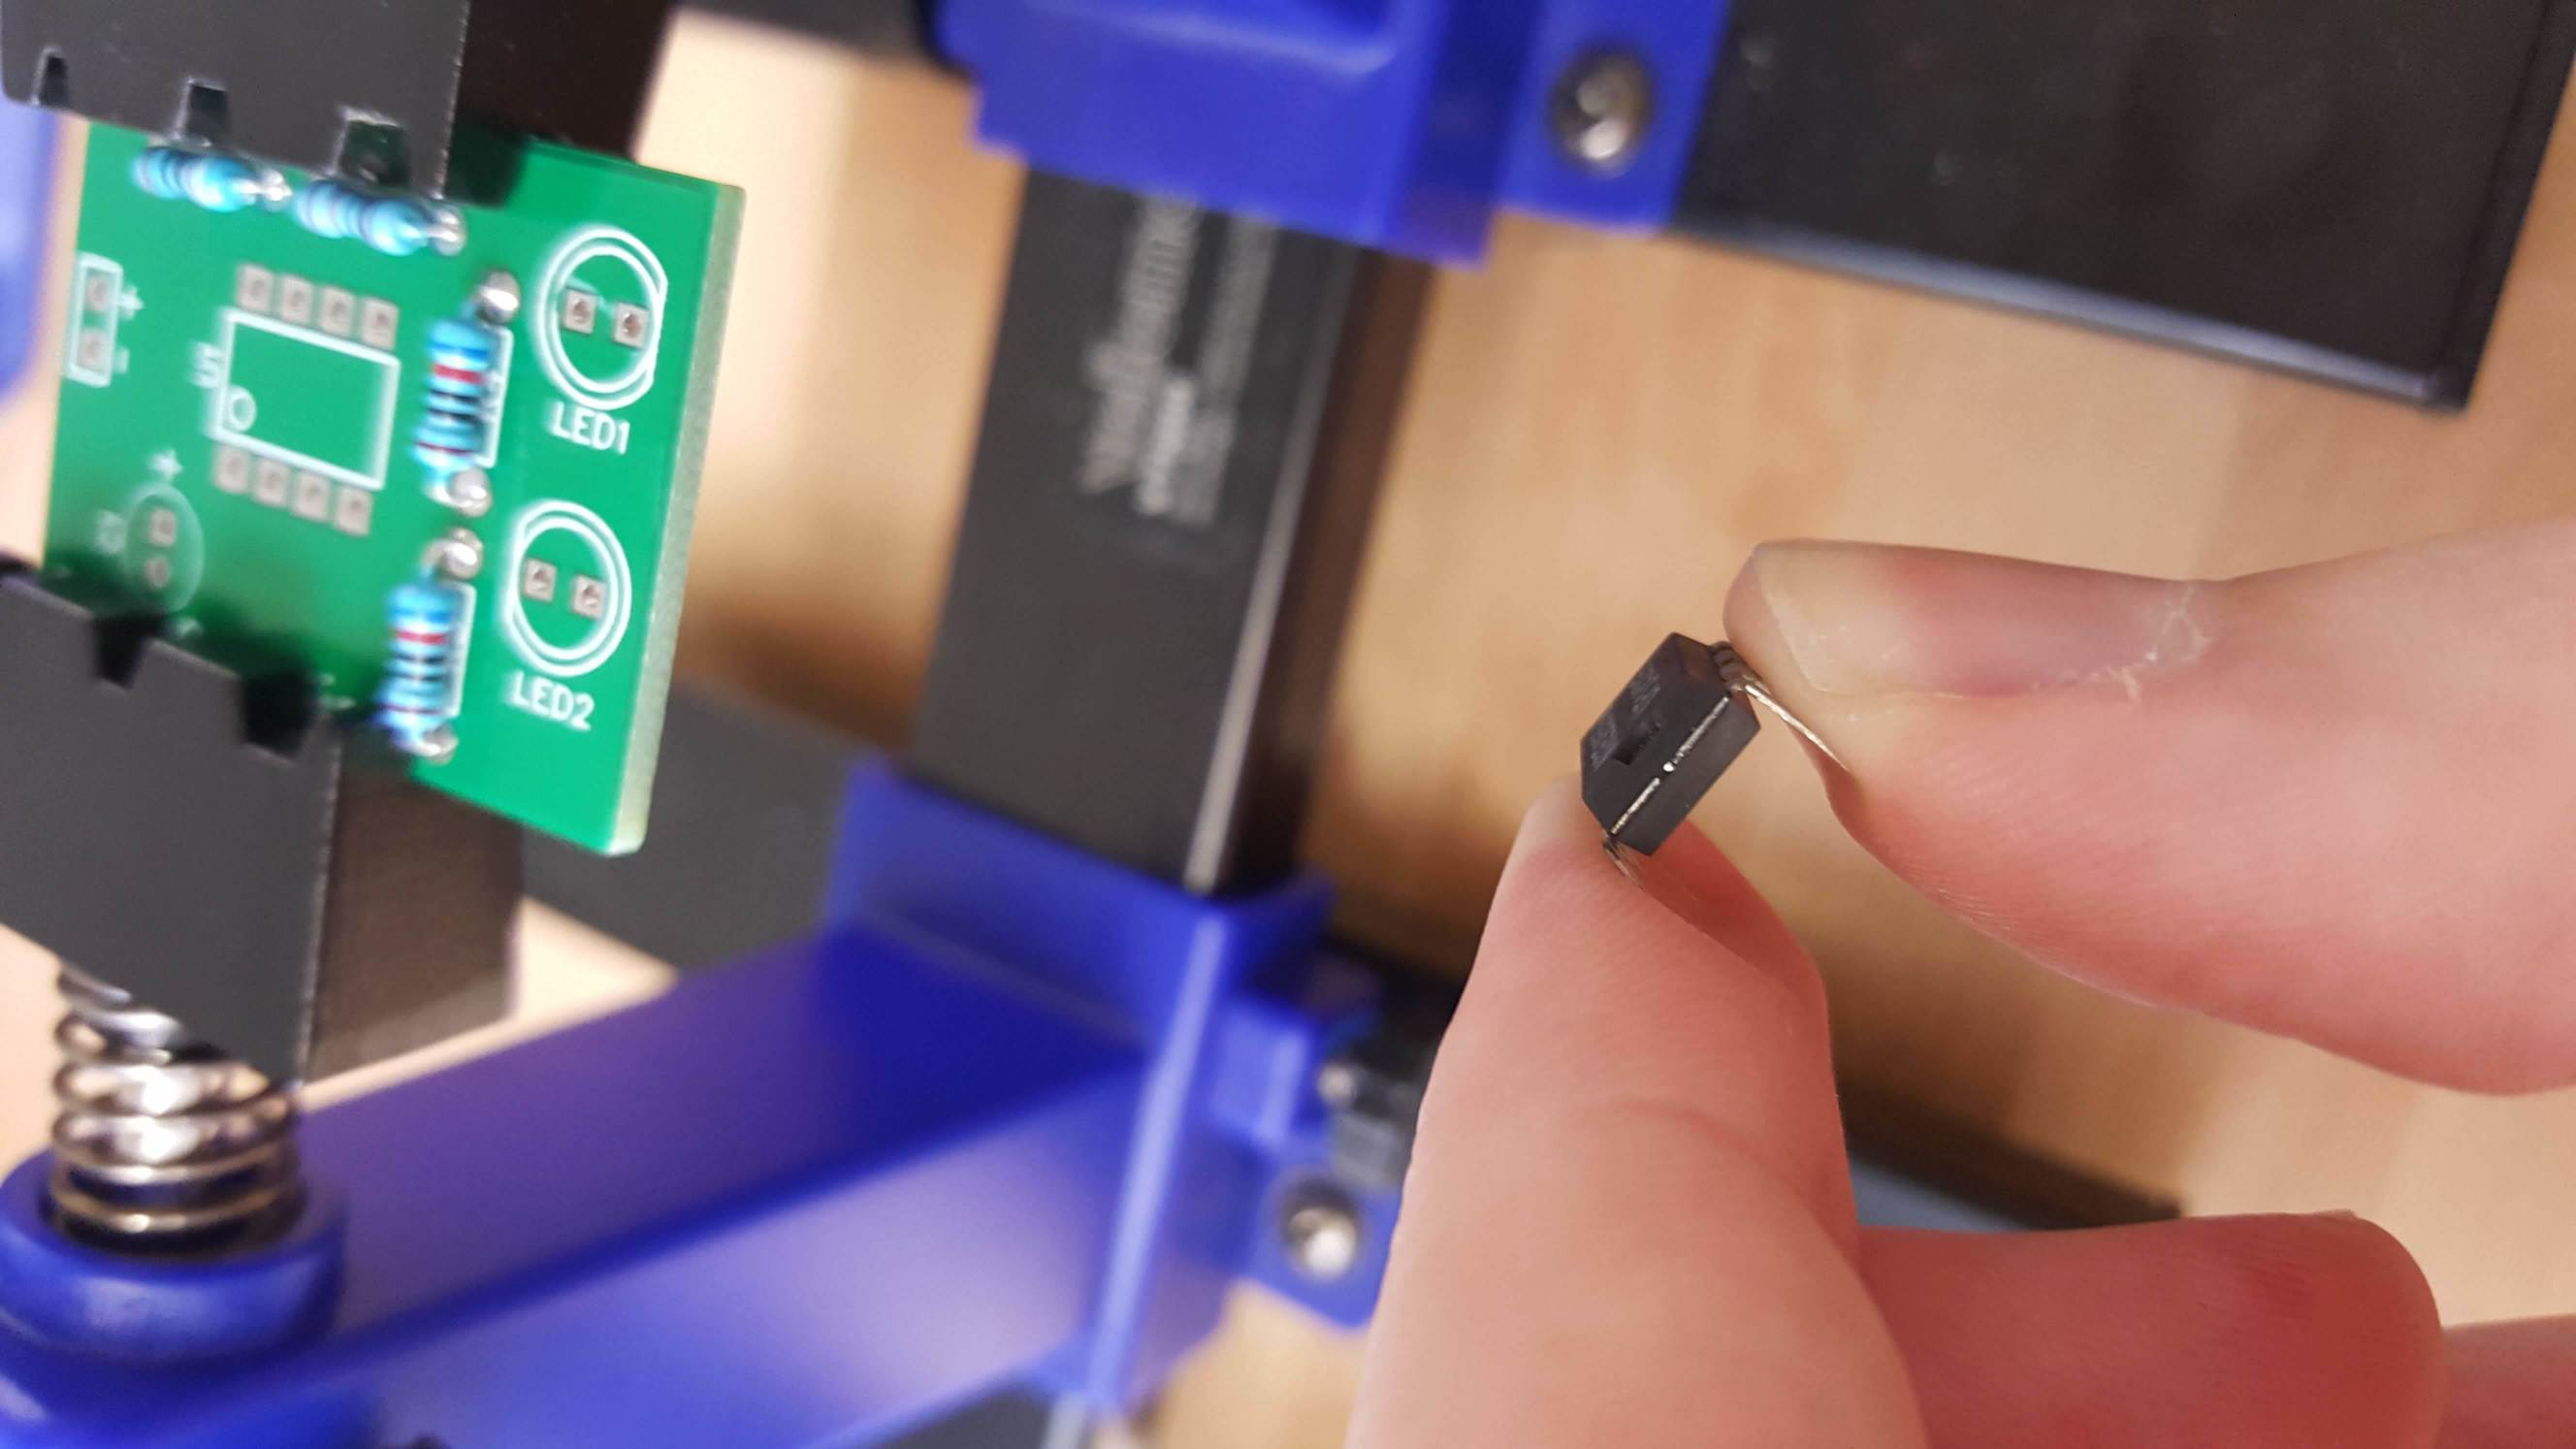
\includegraphics[width=0.75\textwidth]{img/0024.jpg}
\end{figure}

      
\begin{figure}[H]
\caption{ Placing the IC with the Notch Aligned with the Dot }
\label{fig:img/0025.jpg}
\centering
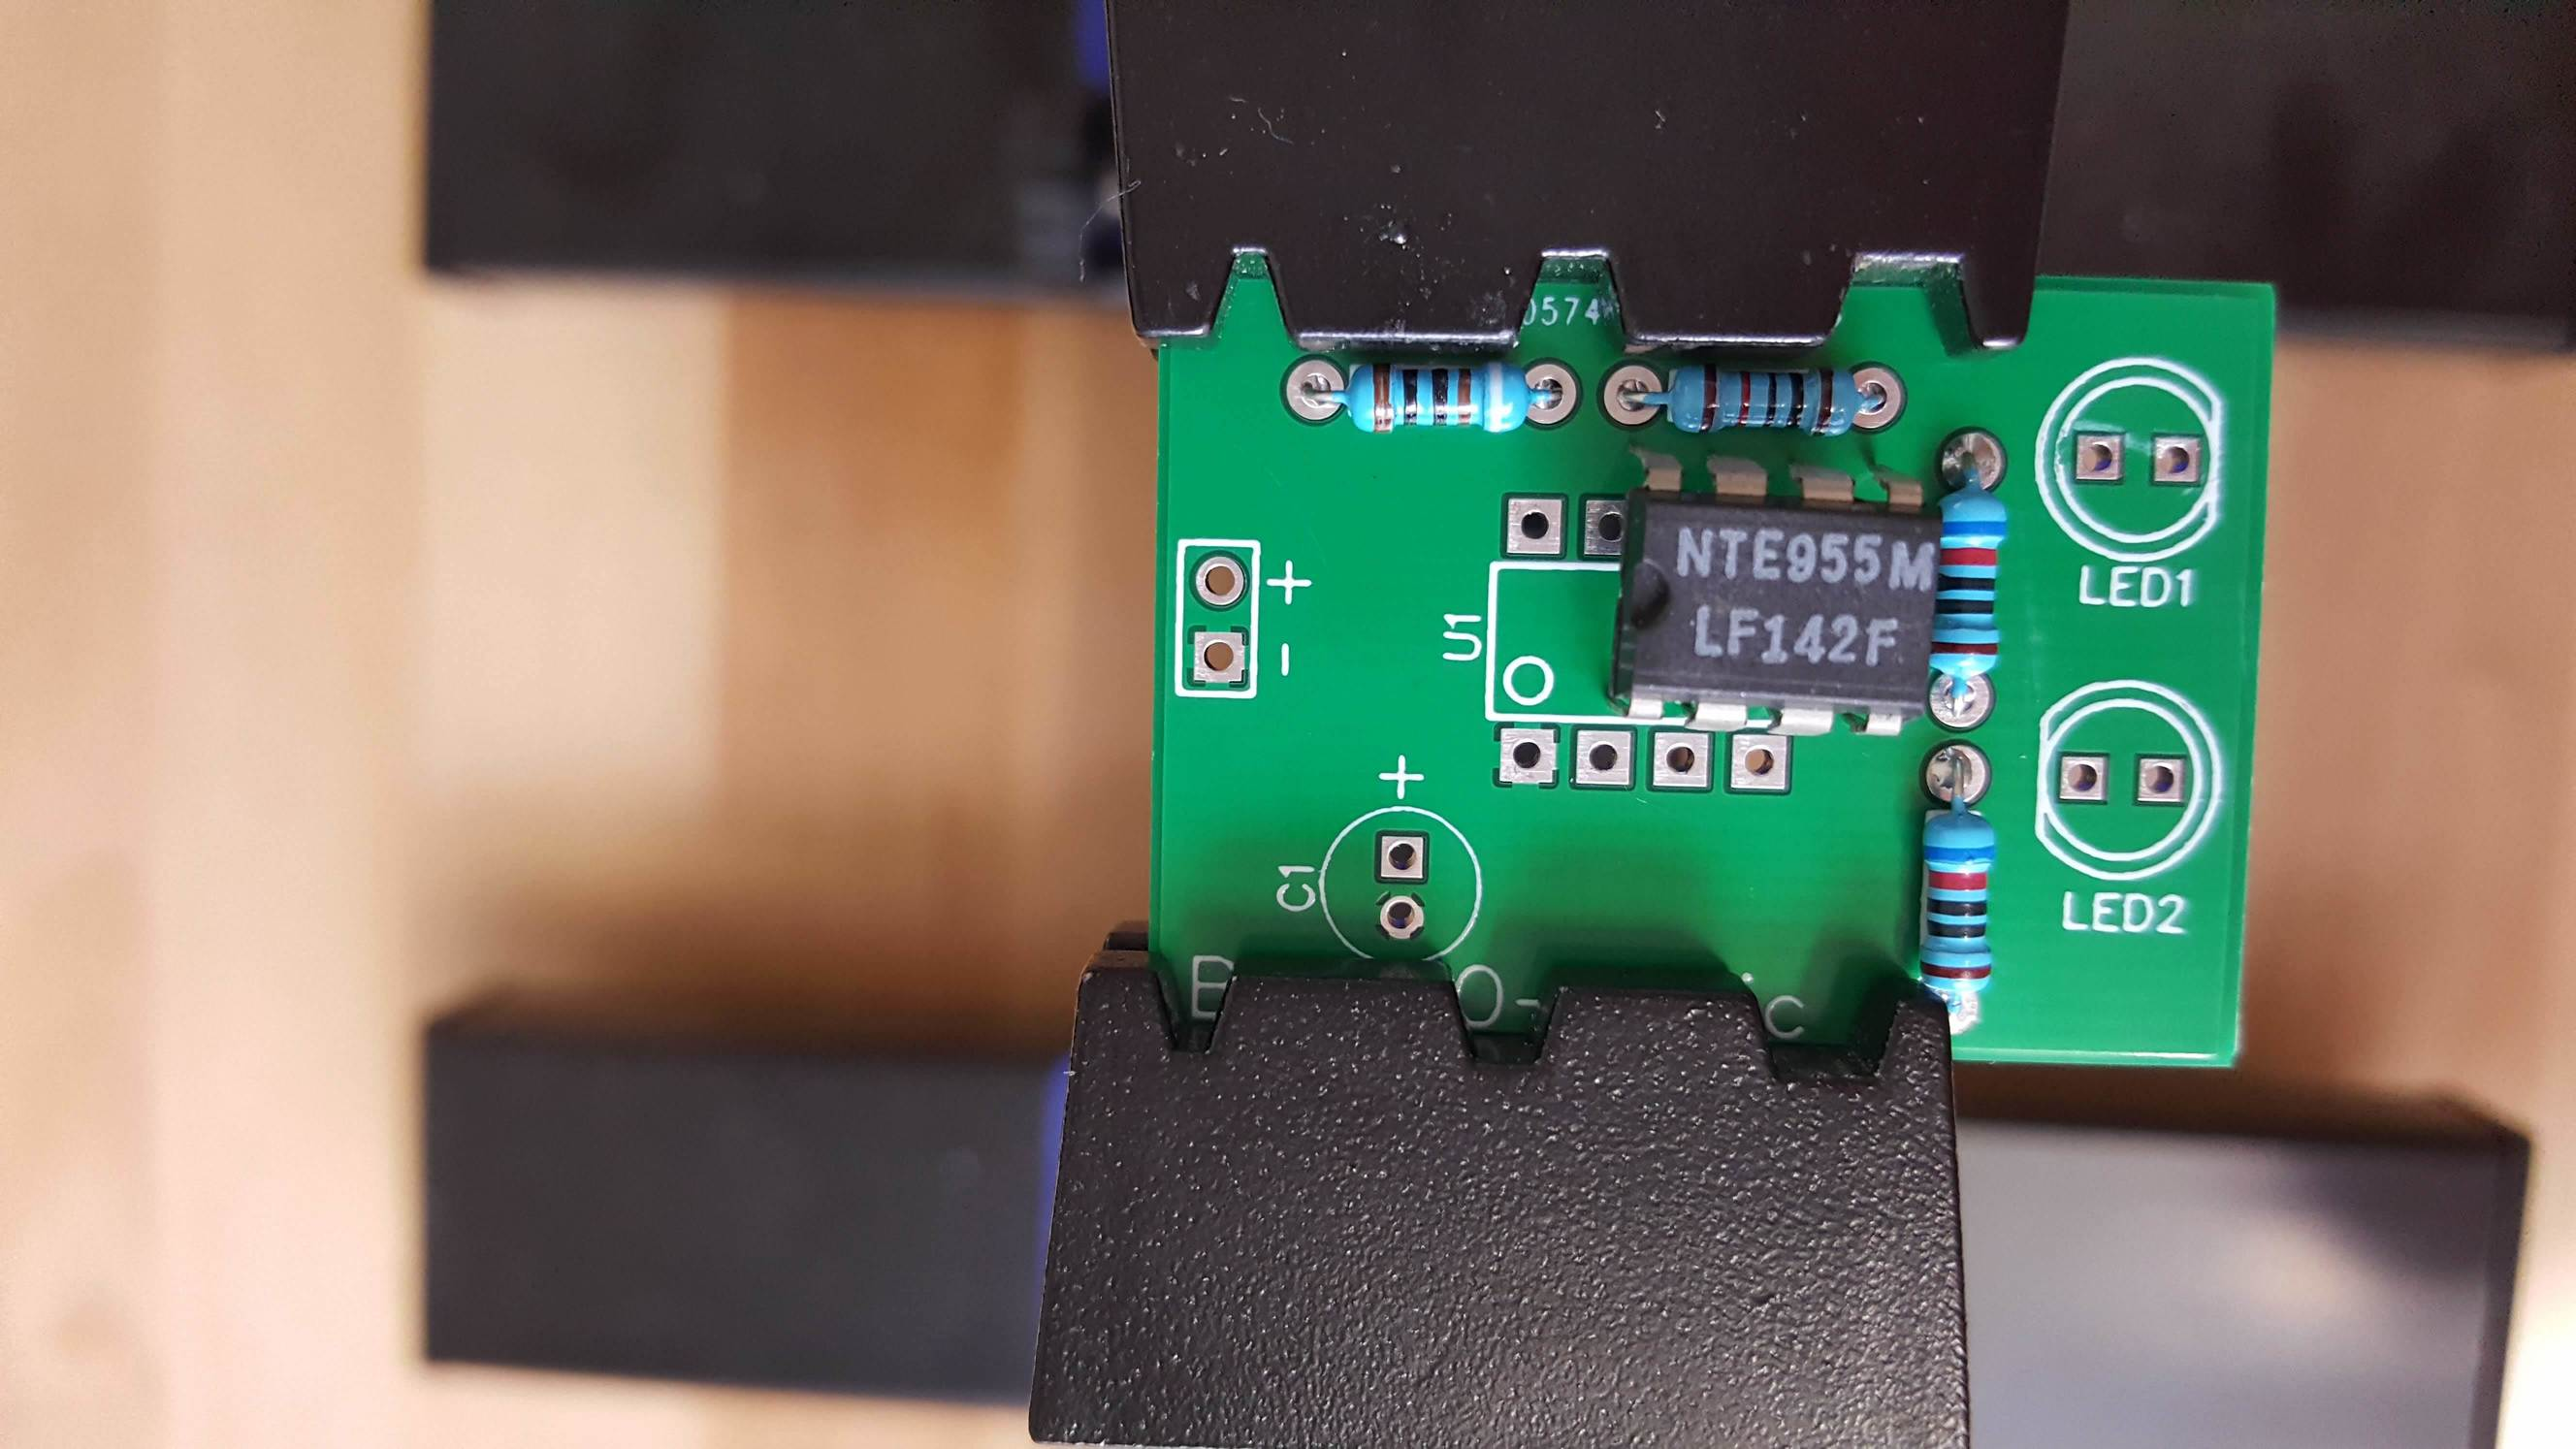
\includegraphics[width=0.75\textwidth]{img/0025.jpg}
\end{figure}

      
\begin{figure}[H]
\caption{ Placing the IC with the Notch Aligned with the Dot }
\label{fig:img/0026.jpg}
\centering
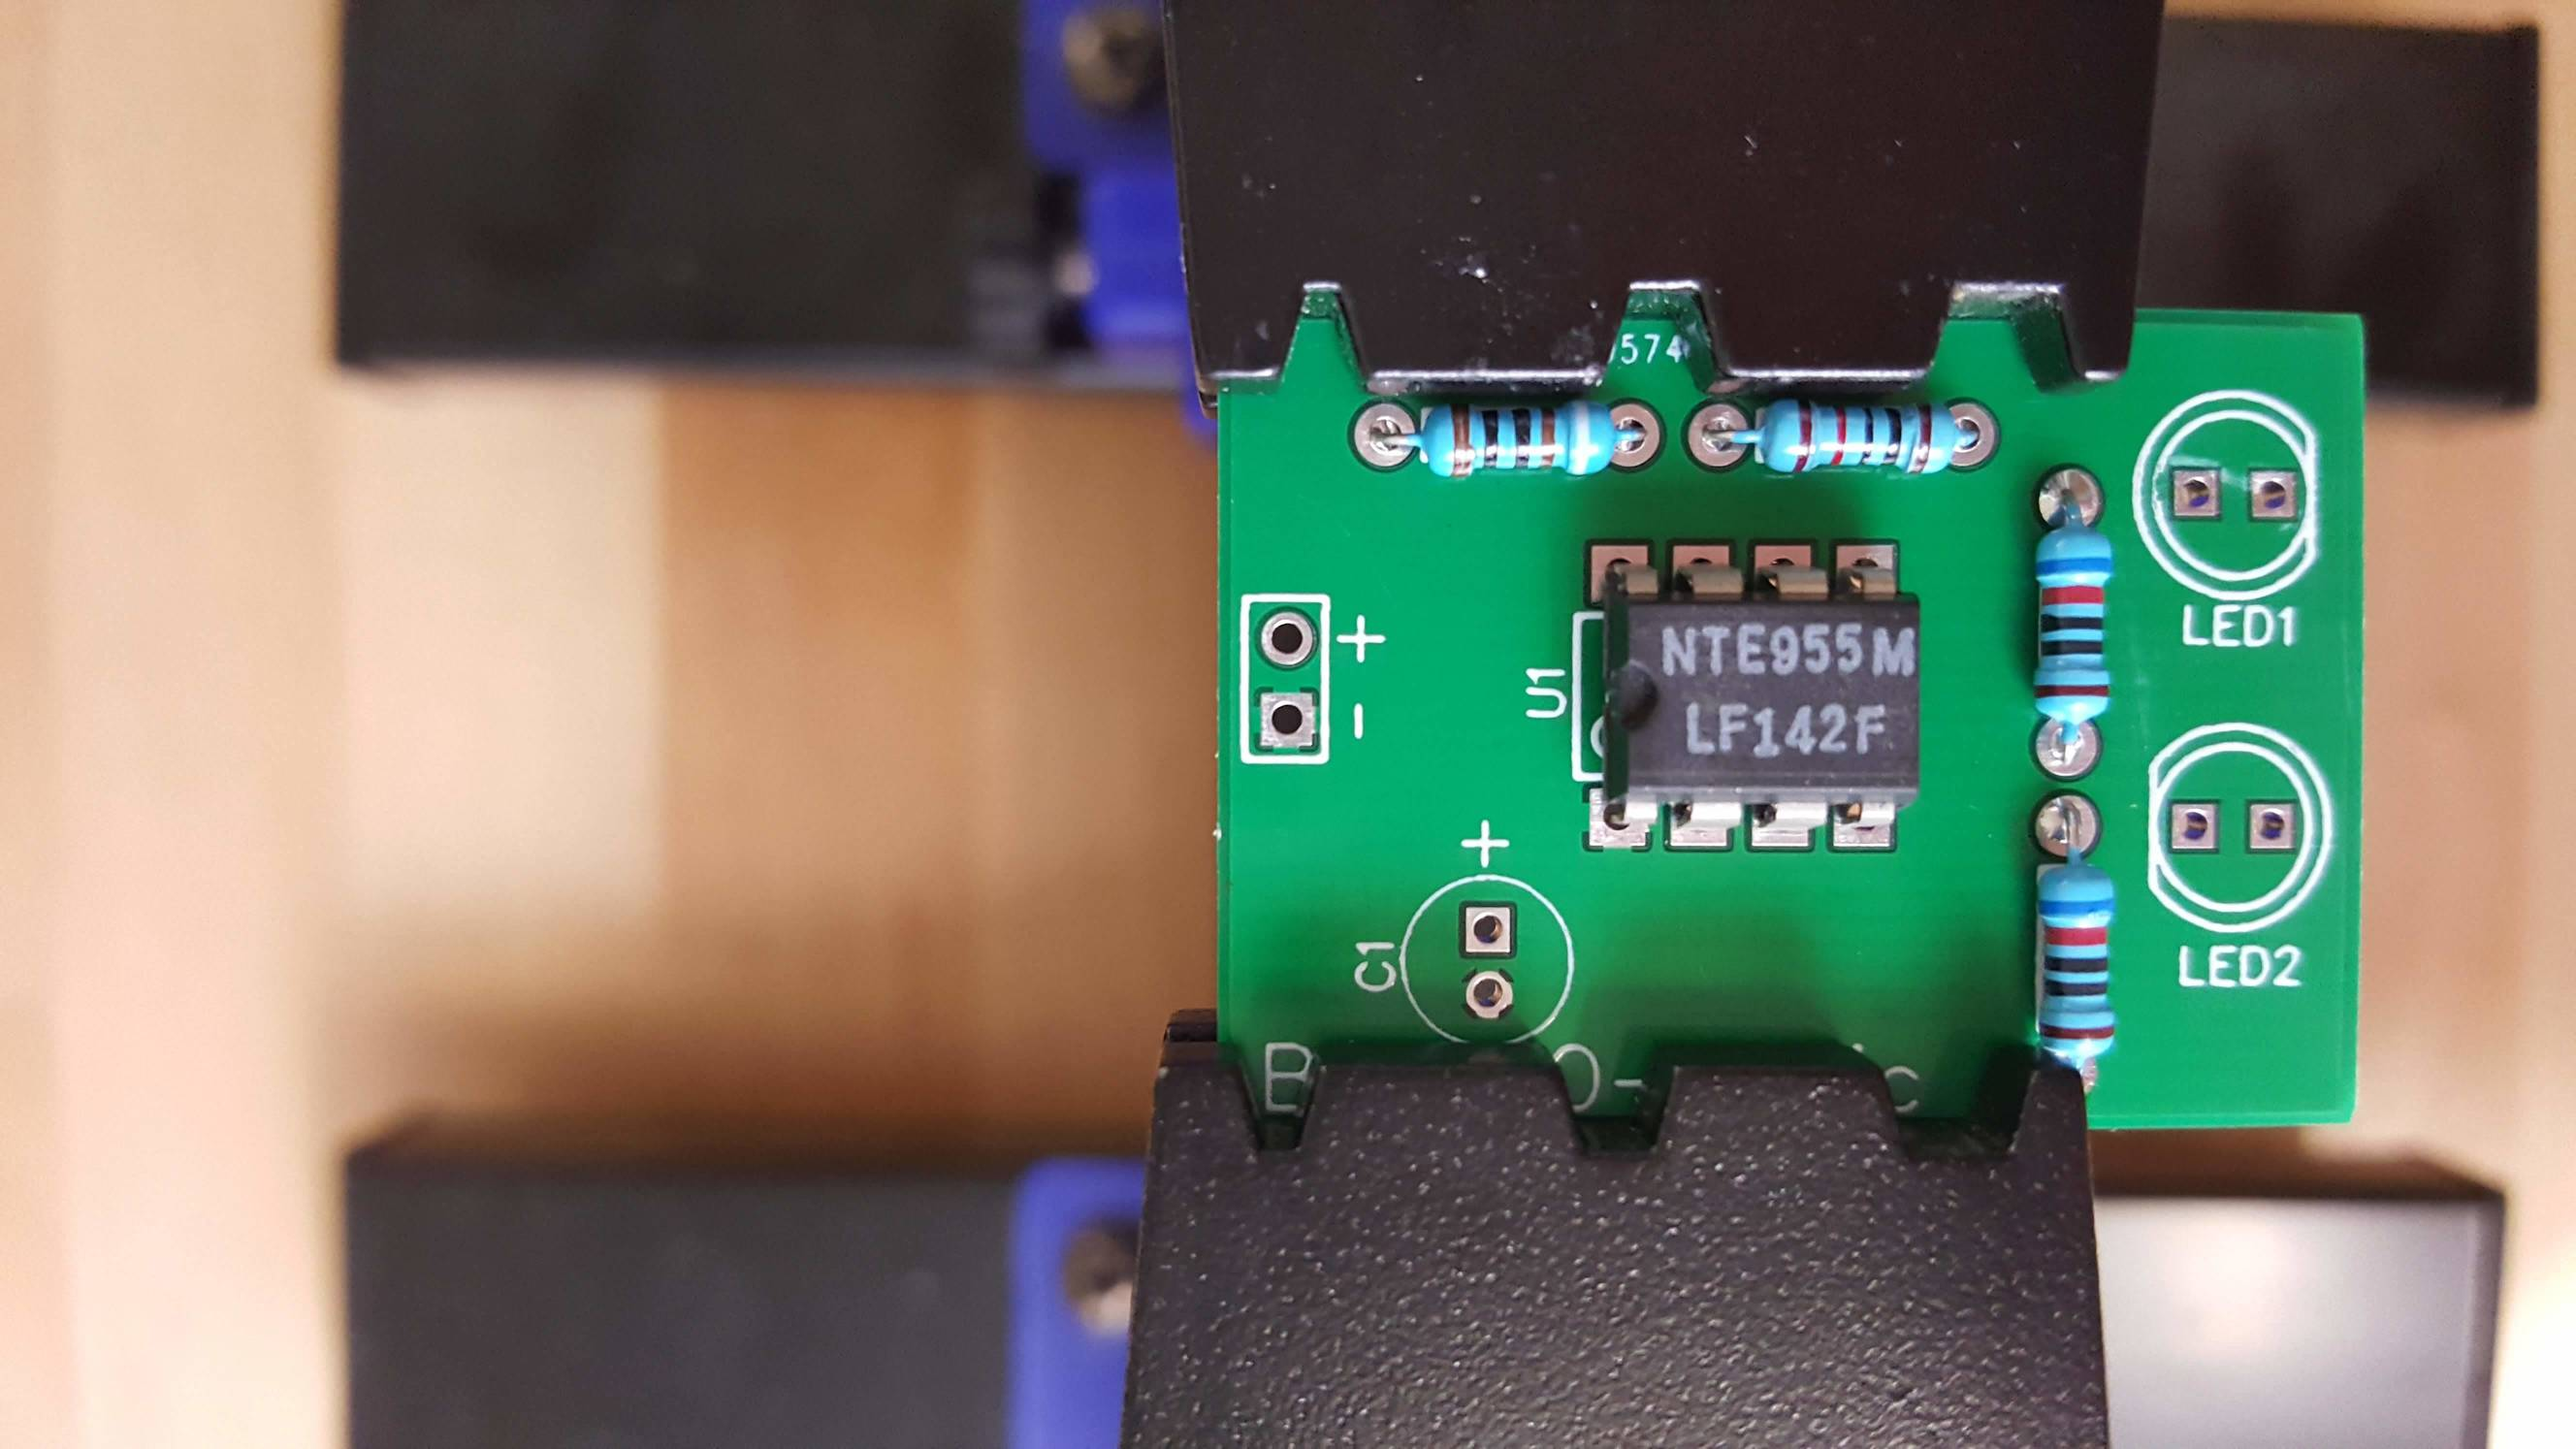
\includegraphics[width=0.75\textwidth]{img/0026.jpg}
\end{figure}

      A method that works well for soldering parts with more than two leads, is to first tack one lead down then put pressure on the part to
      flatten it while brefly applying heat to the joint. This allow the part to be placed as straight as possible. Once it is in the desired spot, the
      remaining pins can be soldered.
      
\begin{figure}[H]
\caption{ One lead being soldered }
\label{fig:img/0029.jpg}
\centering
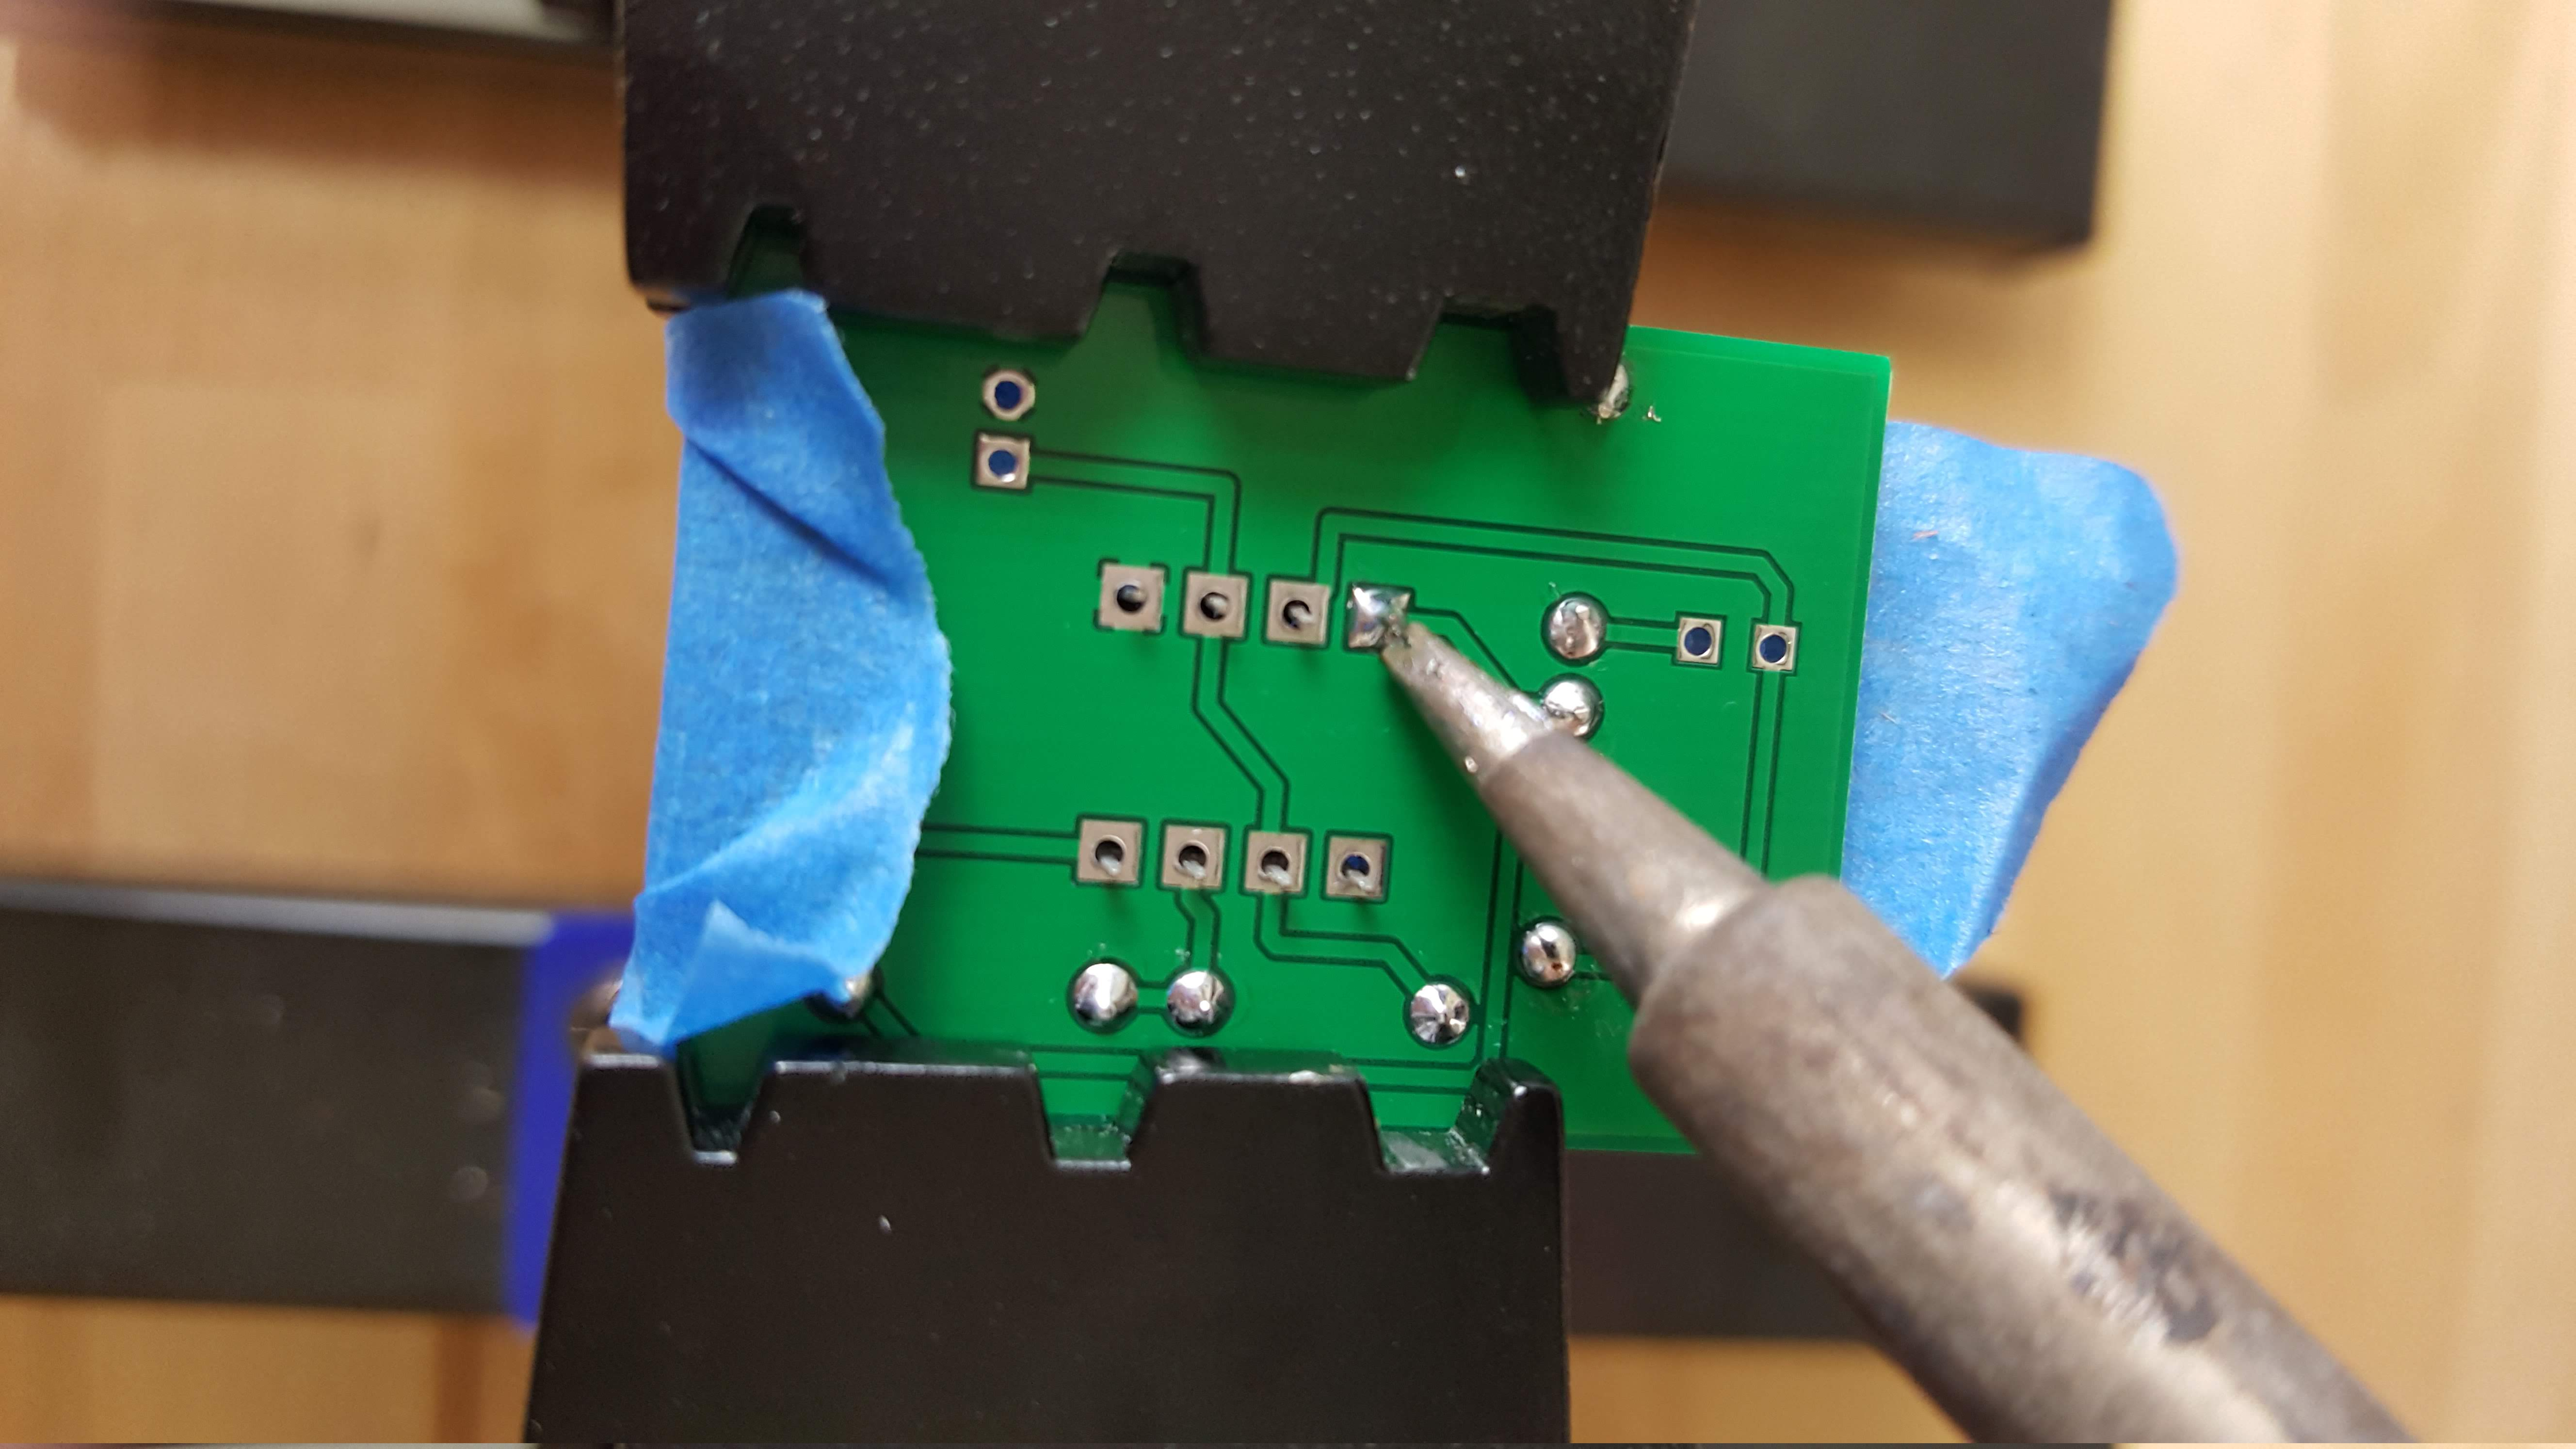
\includegraphics[width=0.75\textwidth]{img/0029.jpg}
\end{figure}

      
\begin{figure}[H]
\caption{ IC being adjusted }
\label{fig:img/0032.jpg}
\centering
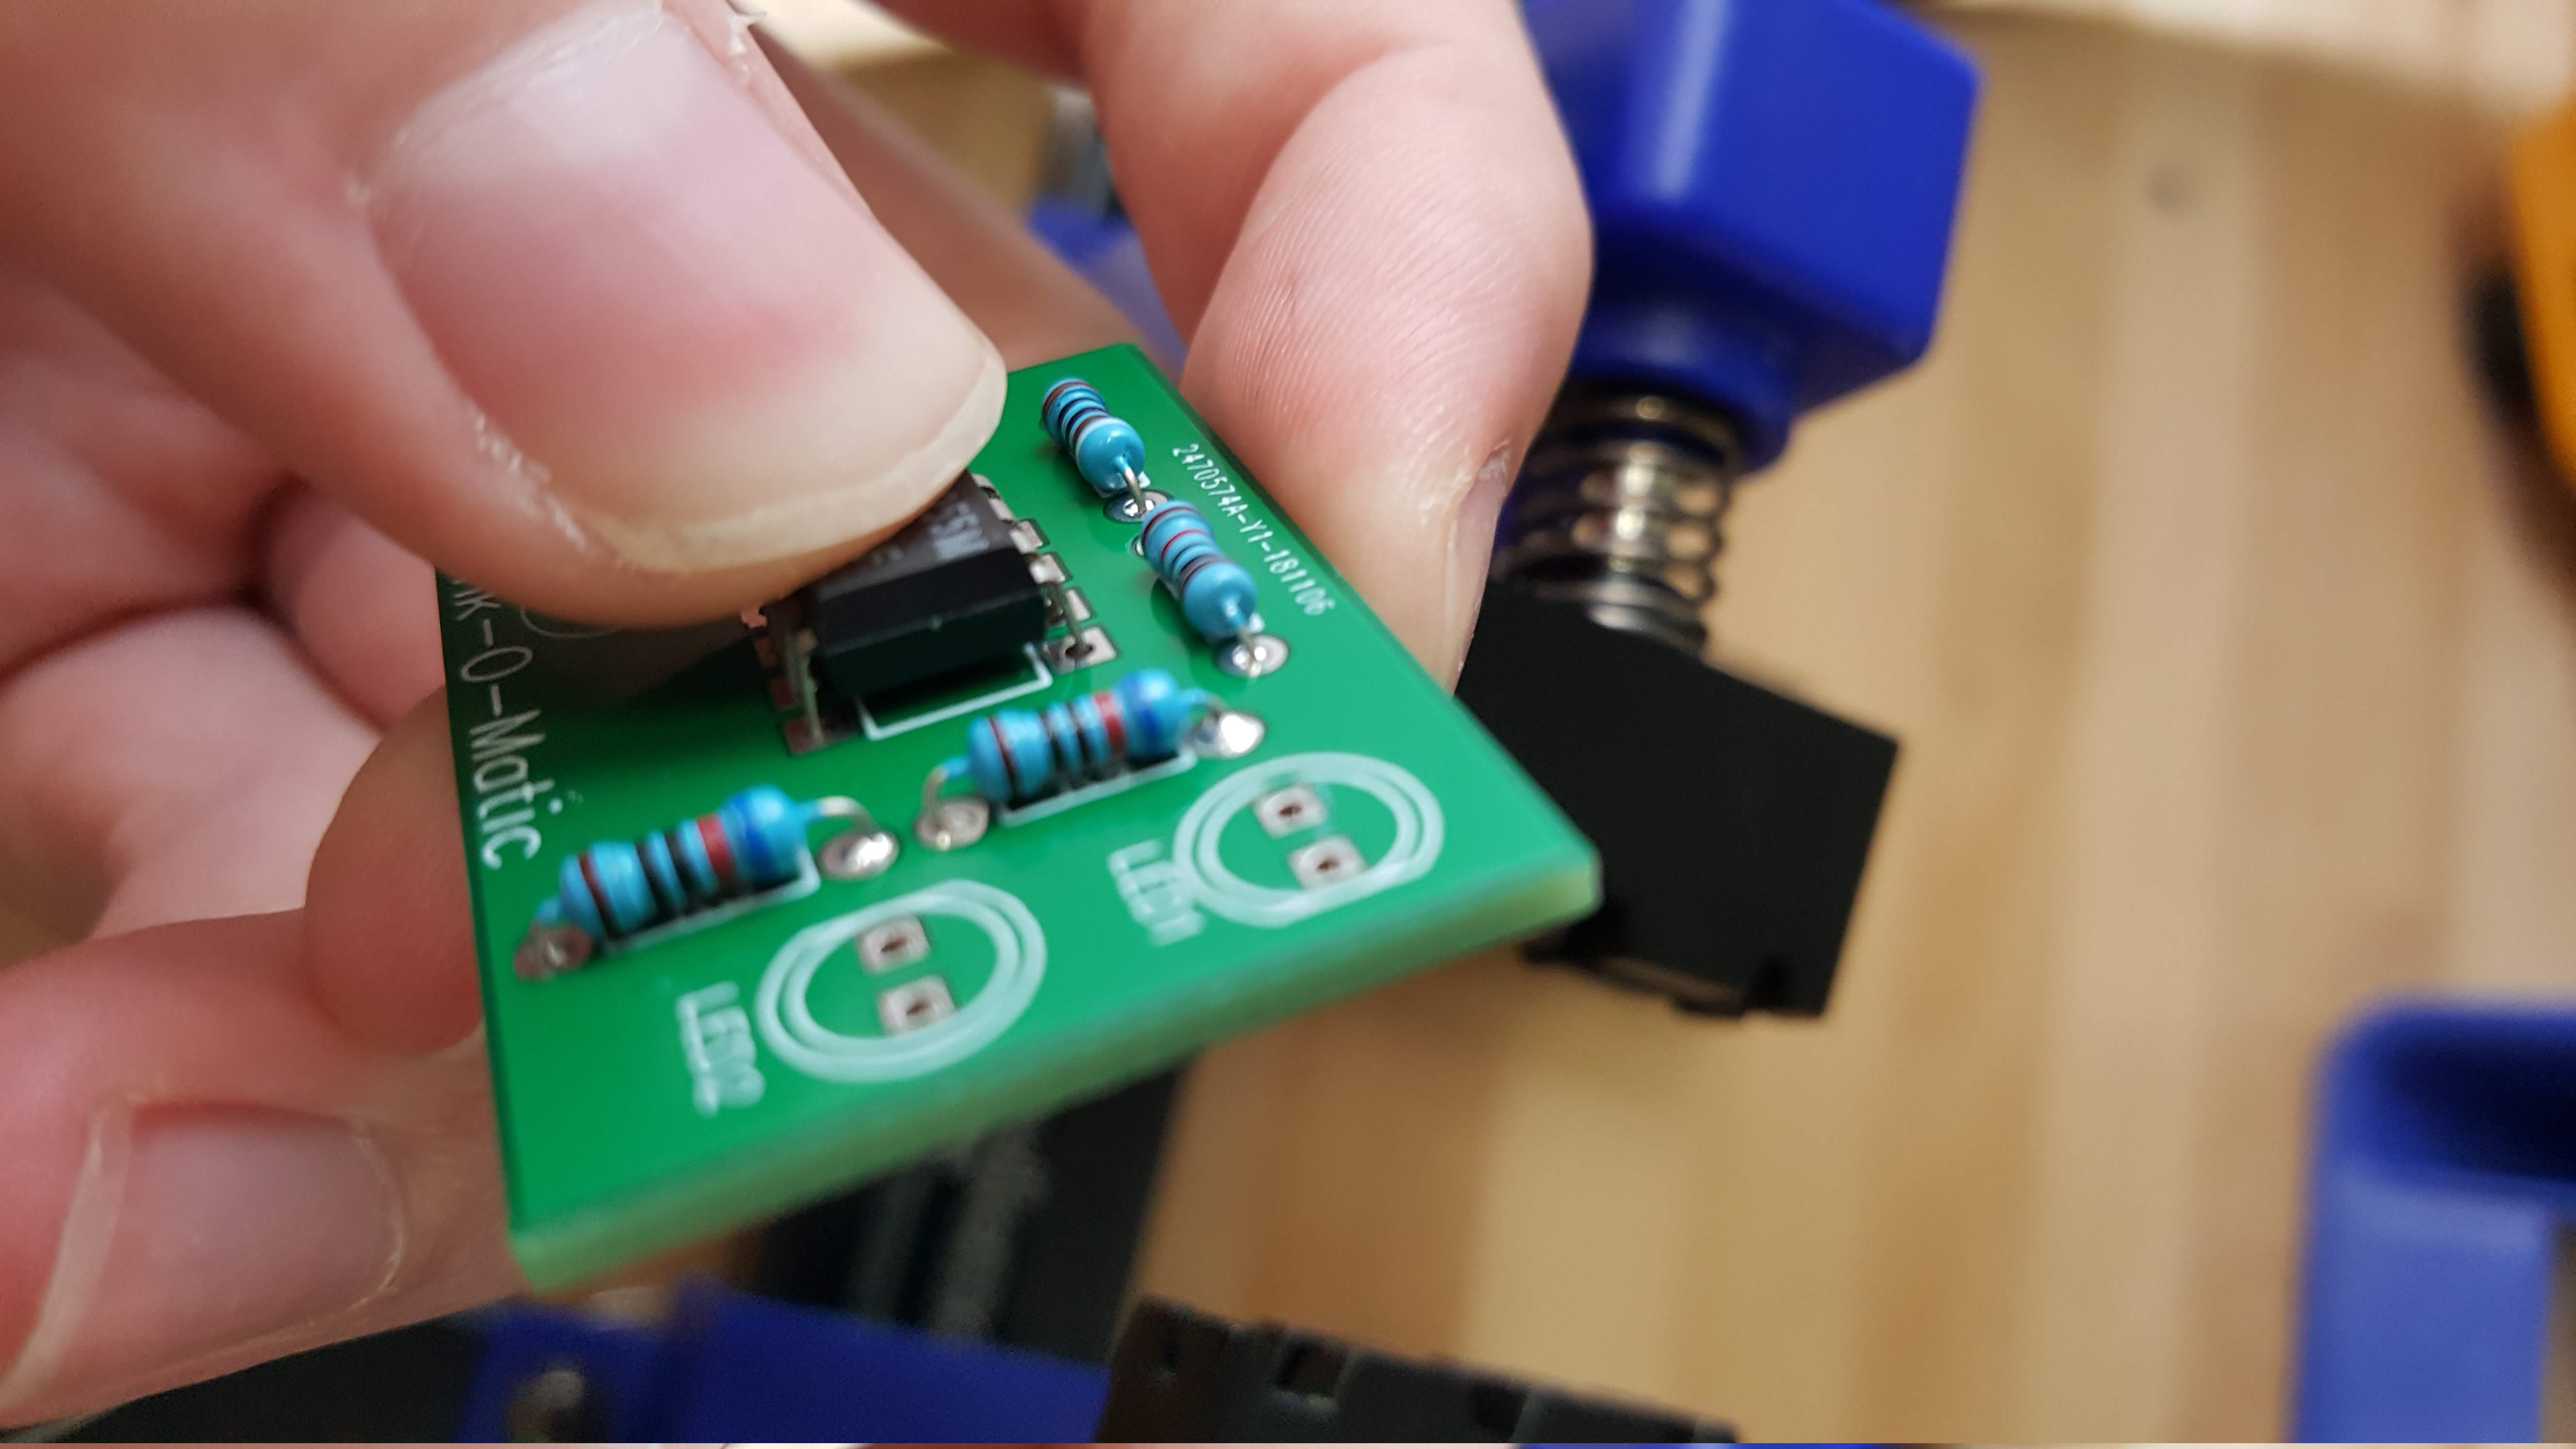
\includegraphics[width=0.75\textwidth]{img/0032.jpg}
\end{figure}

      
\begin{figure}[H]
\caption{ Remaining pins soldered }
\label{fig:img/0033.jpg}
\centering
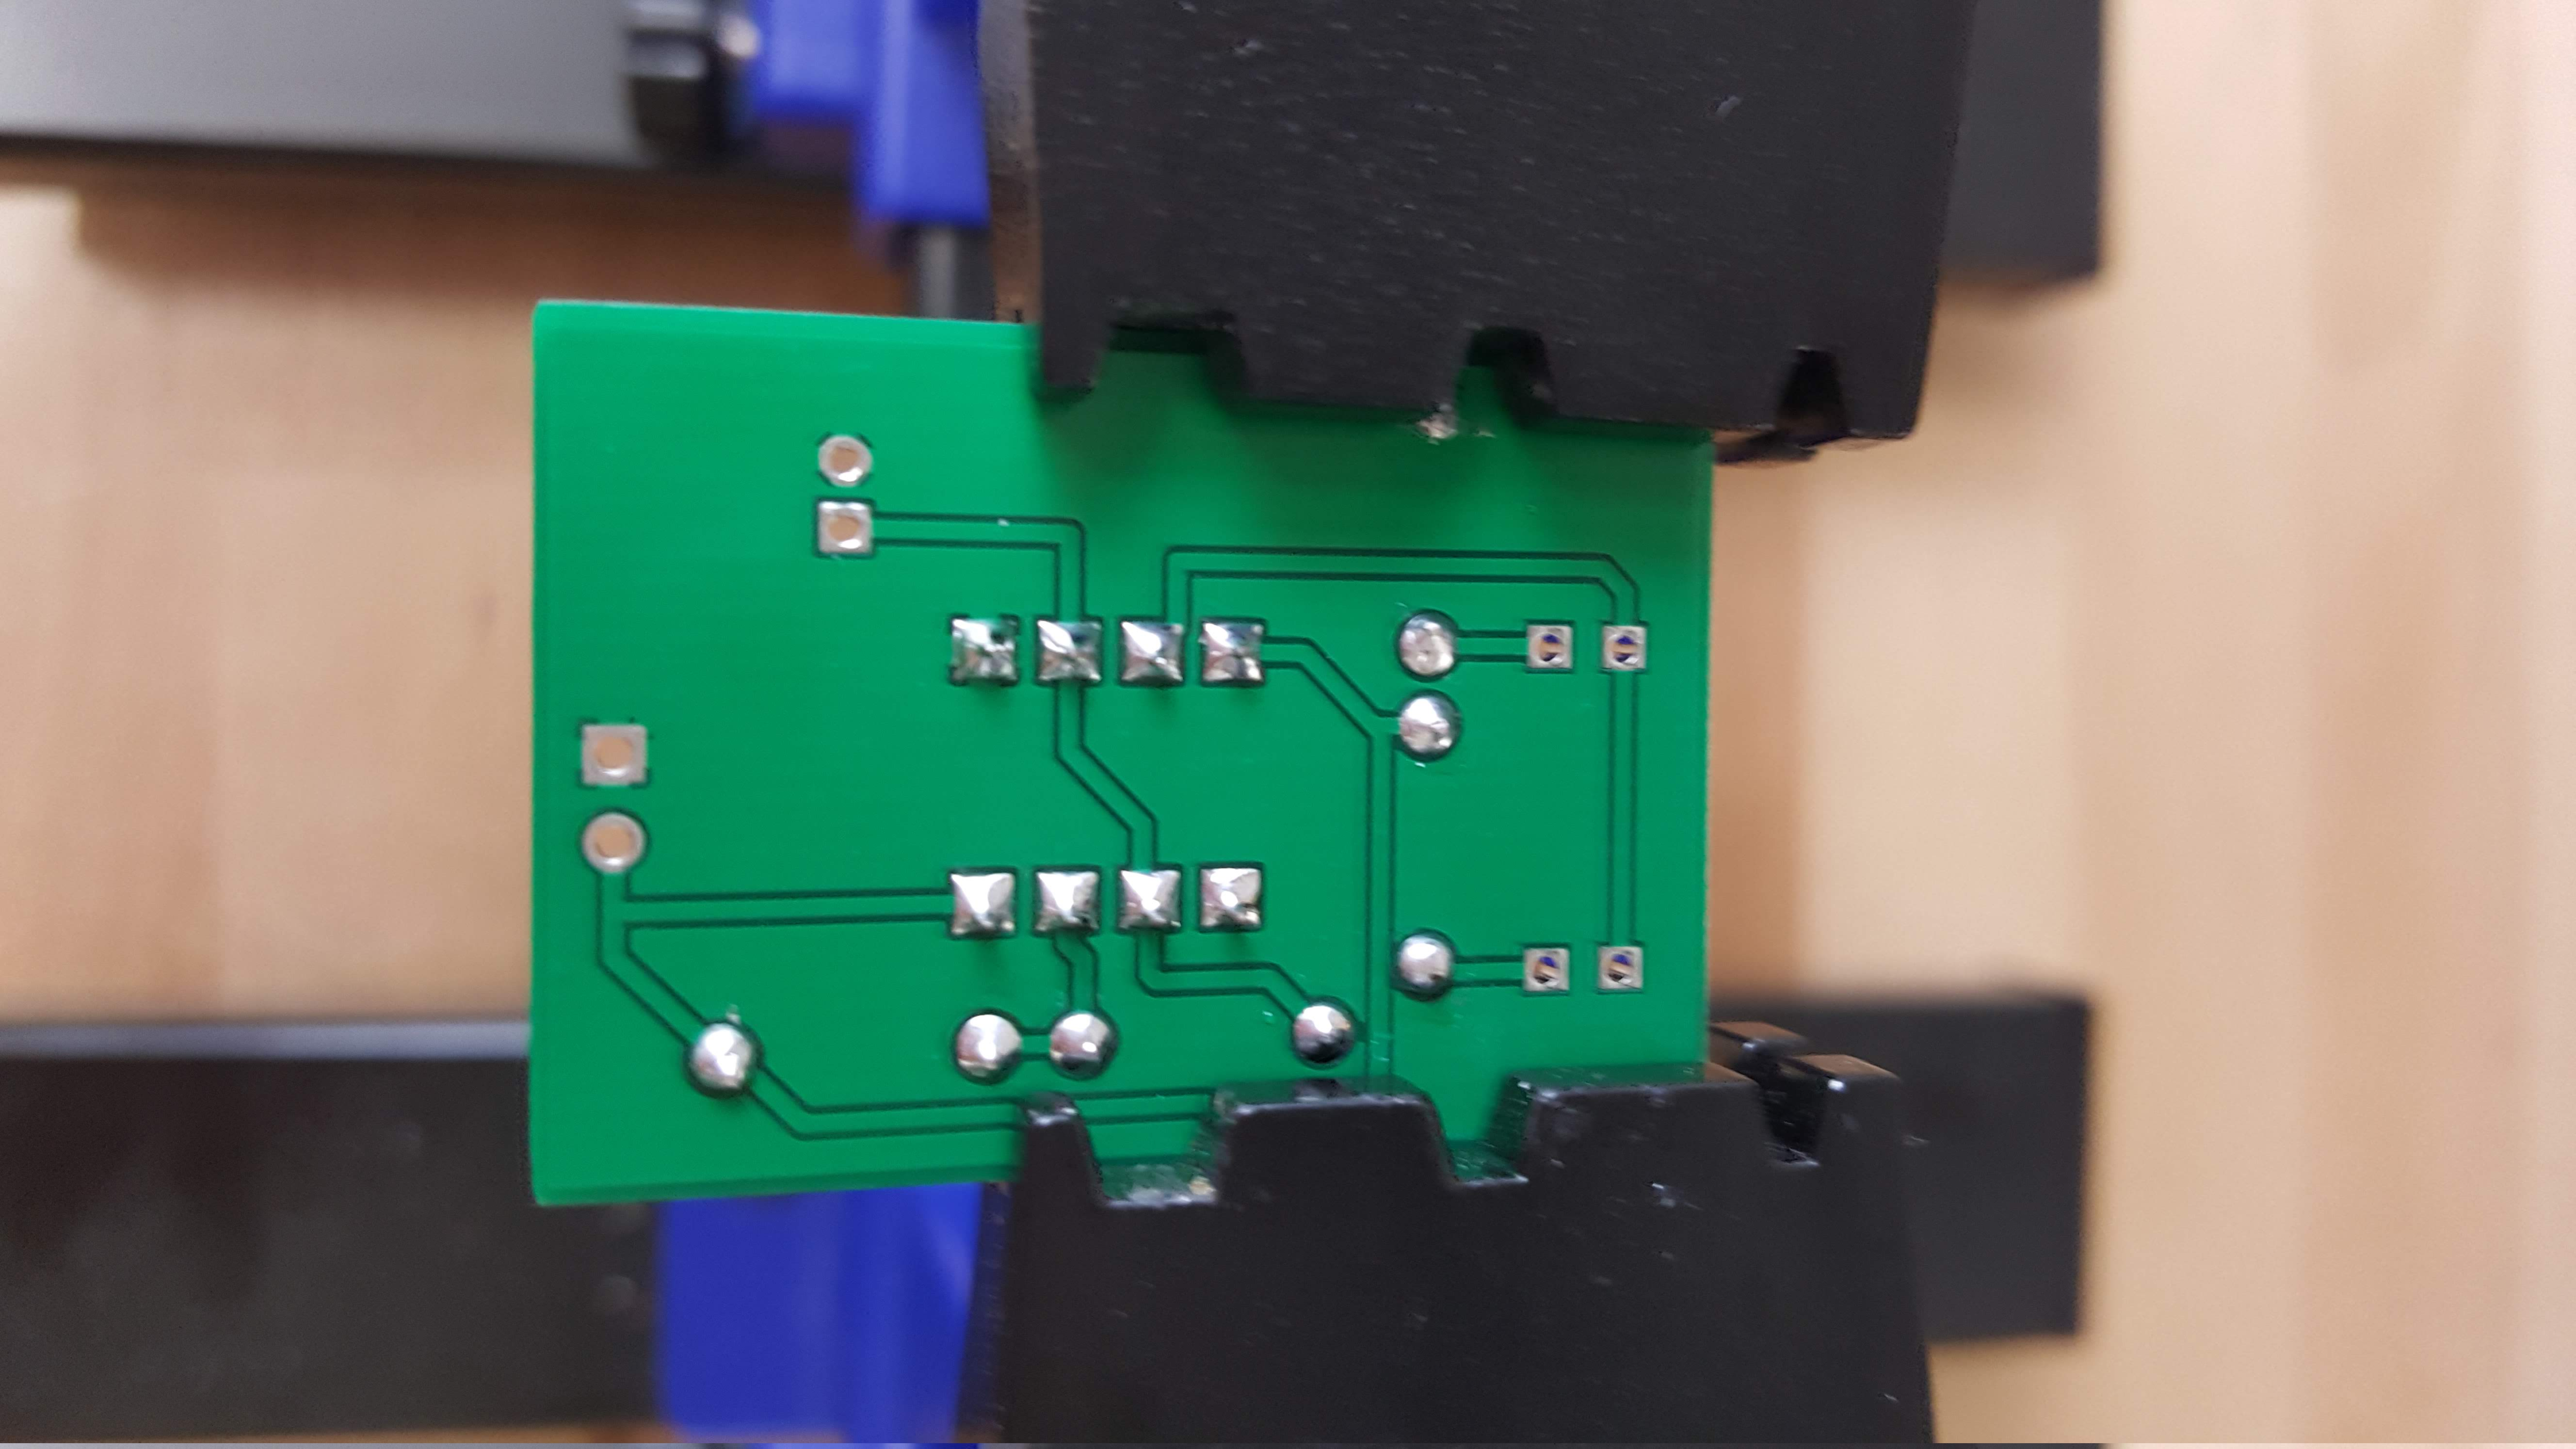
\includegraphics[width=0.75\textwidth]{img/0033.jpg}
\end{figure}

      \item  Now capacitor C1 needs to be soldered. Since these capacitors are polarized they need to be inserted in the correct orientation.
       On the package for the capacitor, it is labeled with a negative sign to indicate
      the negative lead. Also the other lead (the positive lead) is longer. When placing it on the board ensure that the positive lead goes in the hole
      labeled with the plus sign. Once the capacitor is in its place, solder it and then snip the leads.
      
\begin{figure}[H]
\caption{ Electrolytic Capacitor (note the negative strip and the longer positive lead) }
\label{fig:img/0035.jpg}
\centering
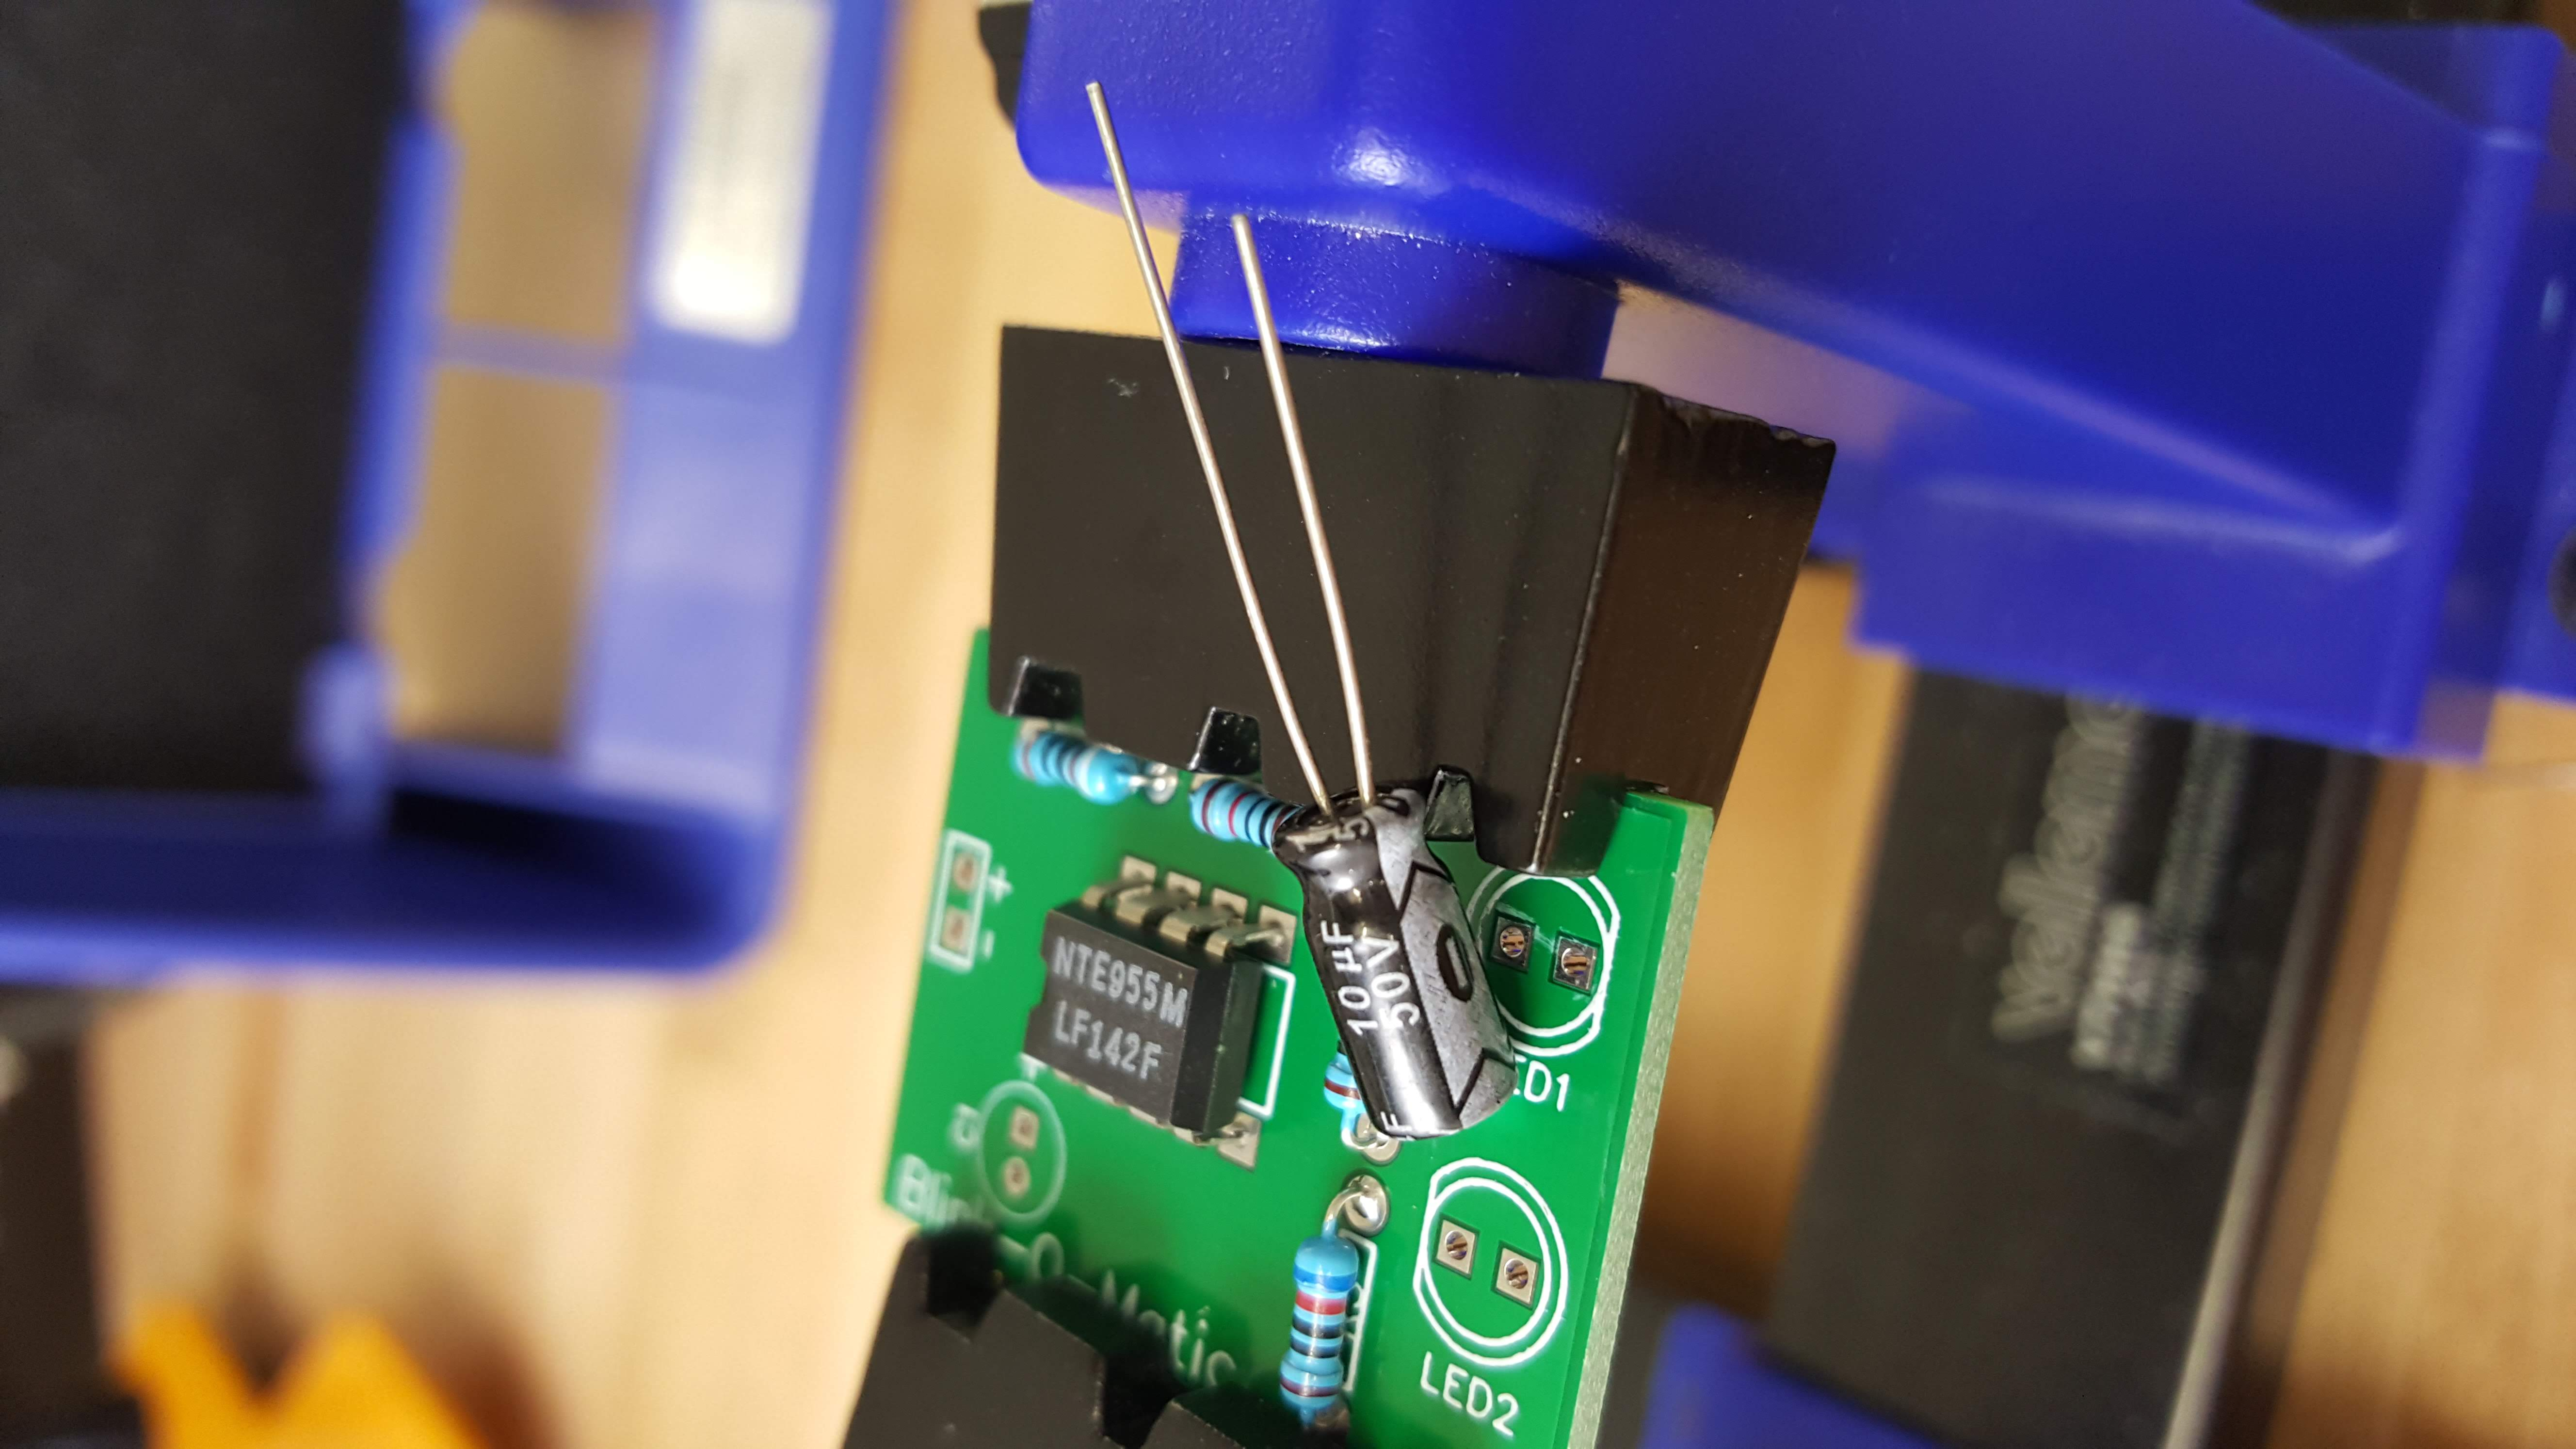
\includegraphics[width=0.75\textwidth]{img/0035.jpg}
\end{figure}

      
\begin{figure}[H]
\caption{ Inserting C1 (being careful of polarity) }
\label{fig:img/0040.jpg}
\centering
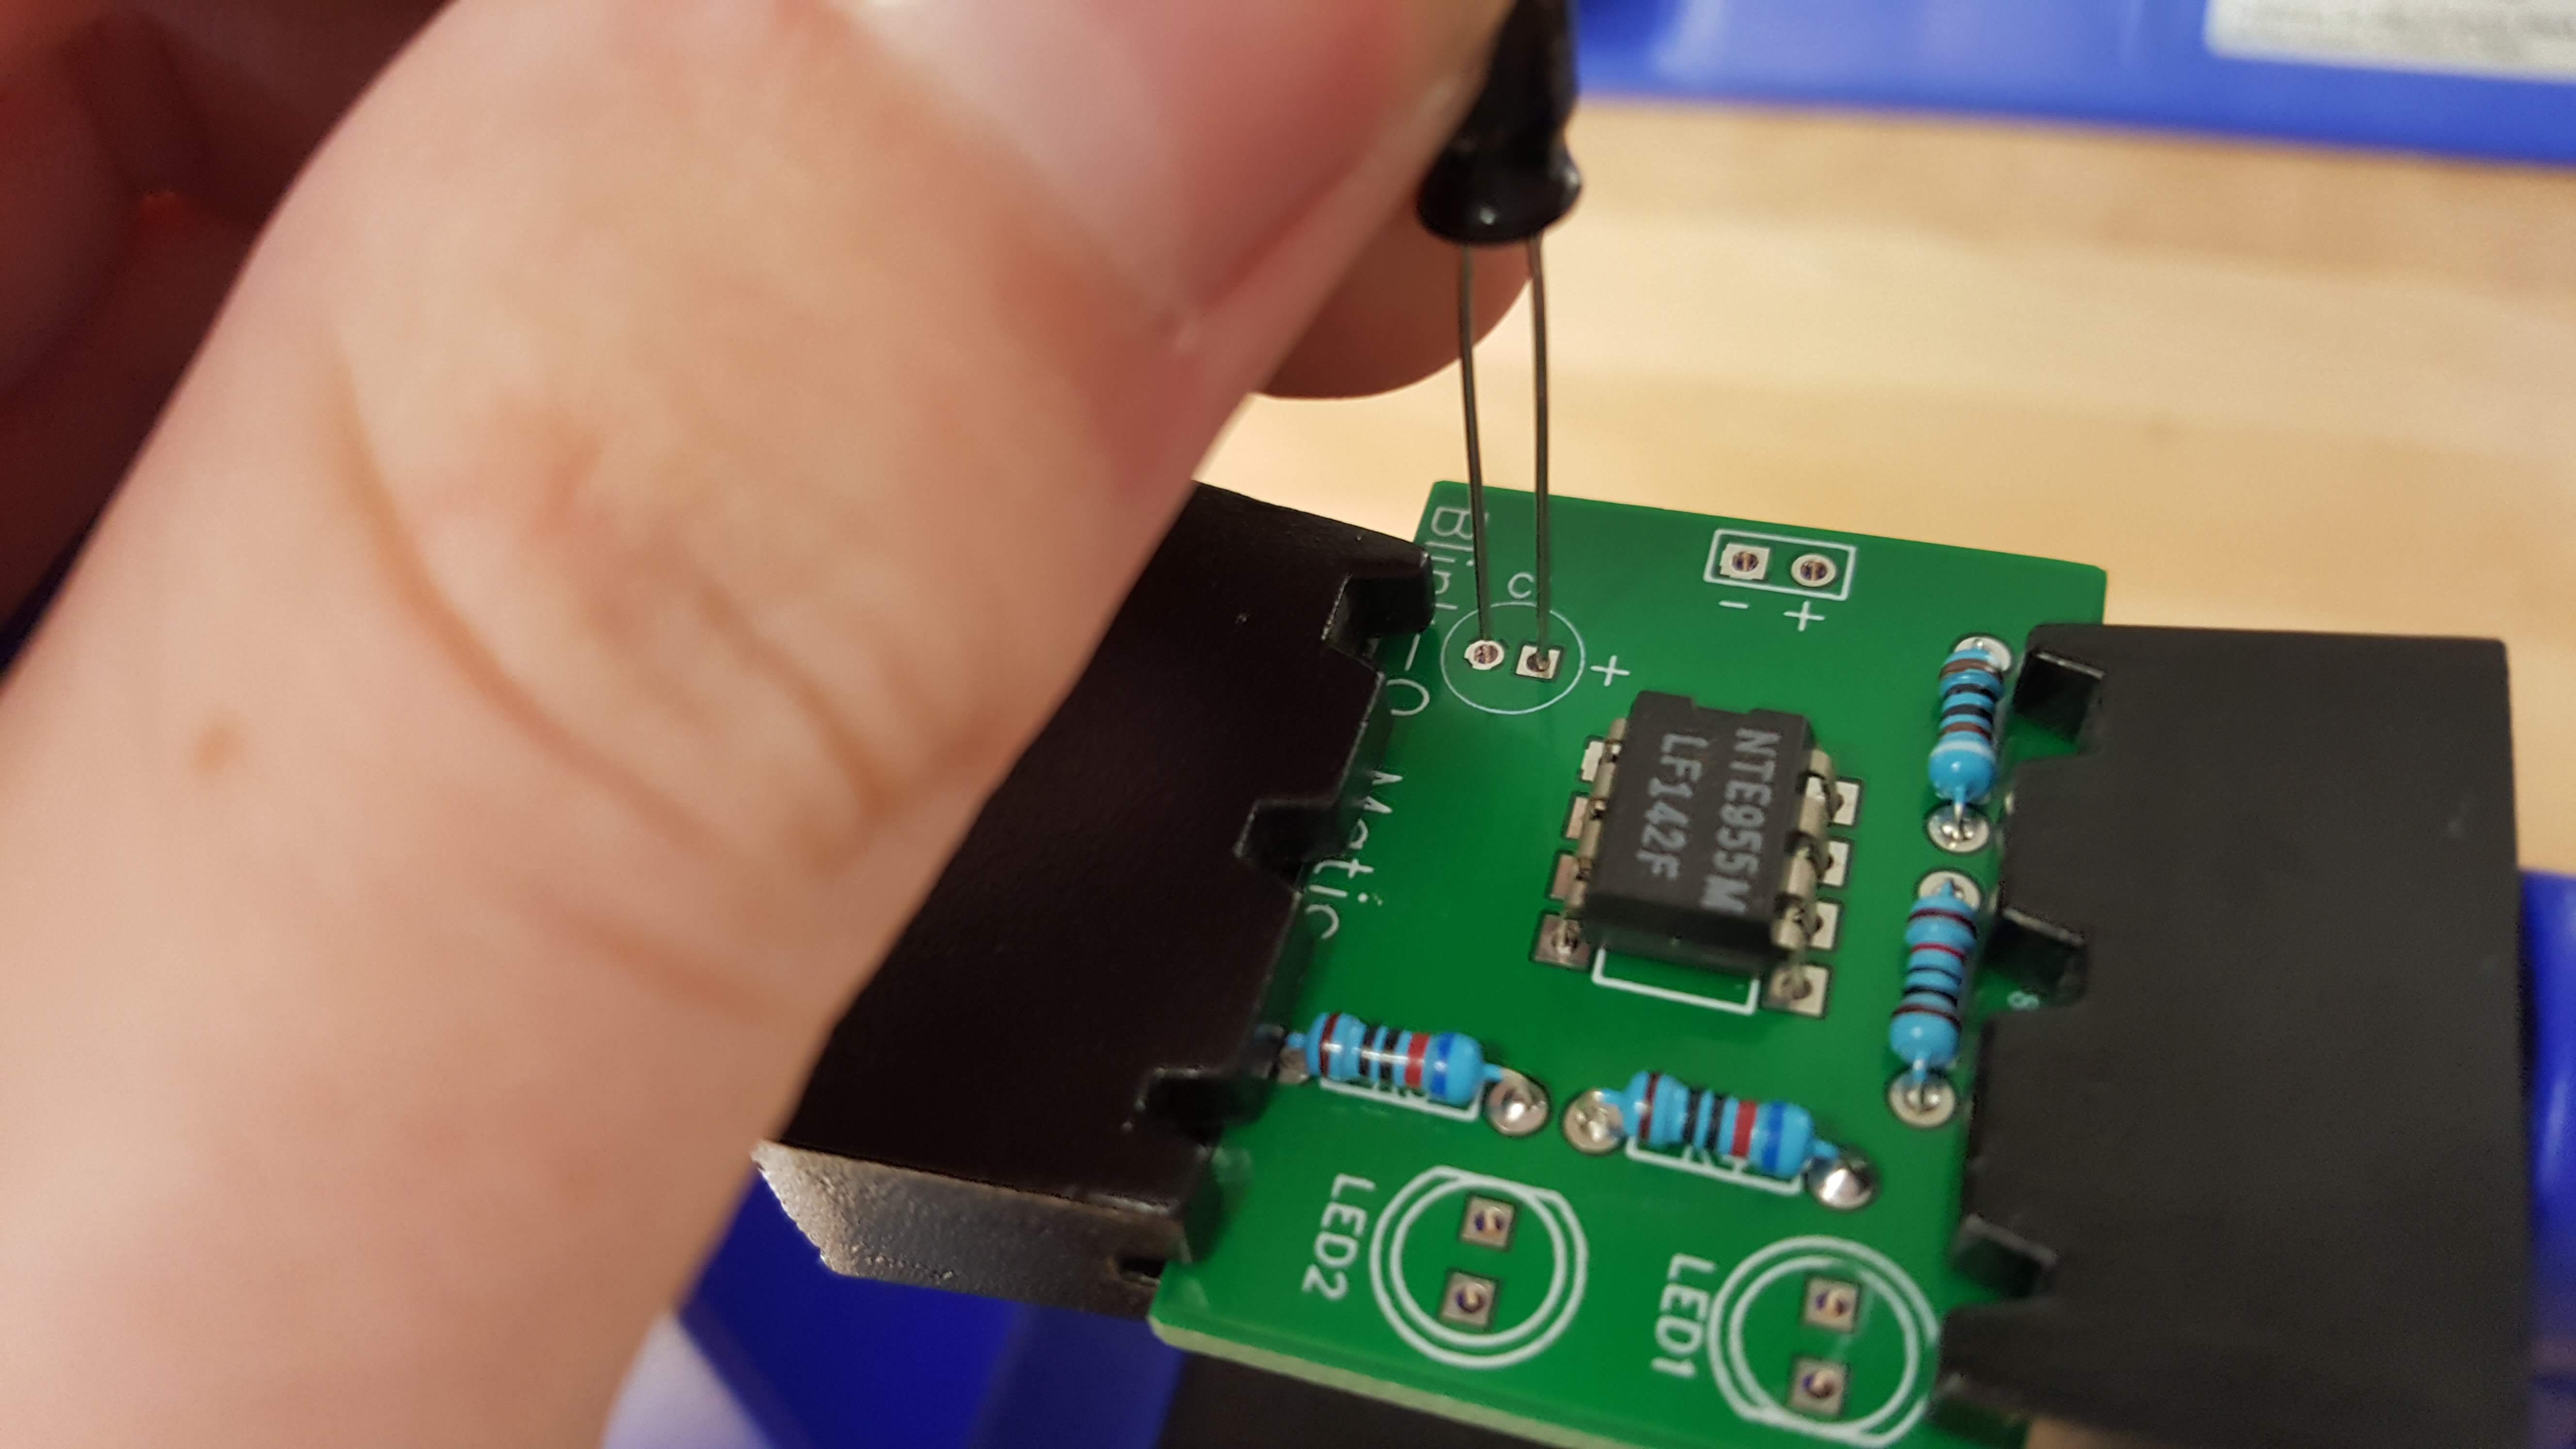
\includegraphics[width=0.75\textwidth]{img/0040.jpg}
\end{figure}

      
\begin{figure}[H]
\caption{ C1 in its Place }
\label{fig:img/0041.jpg}
\centering
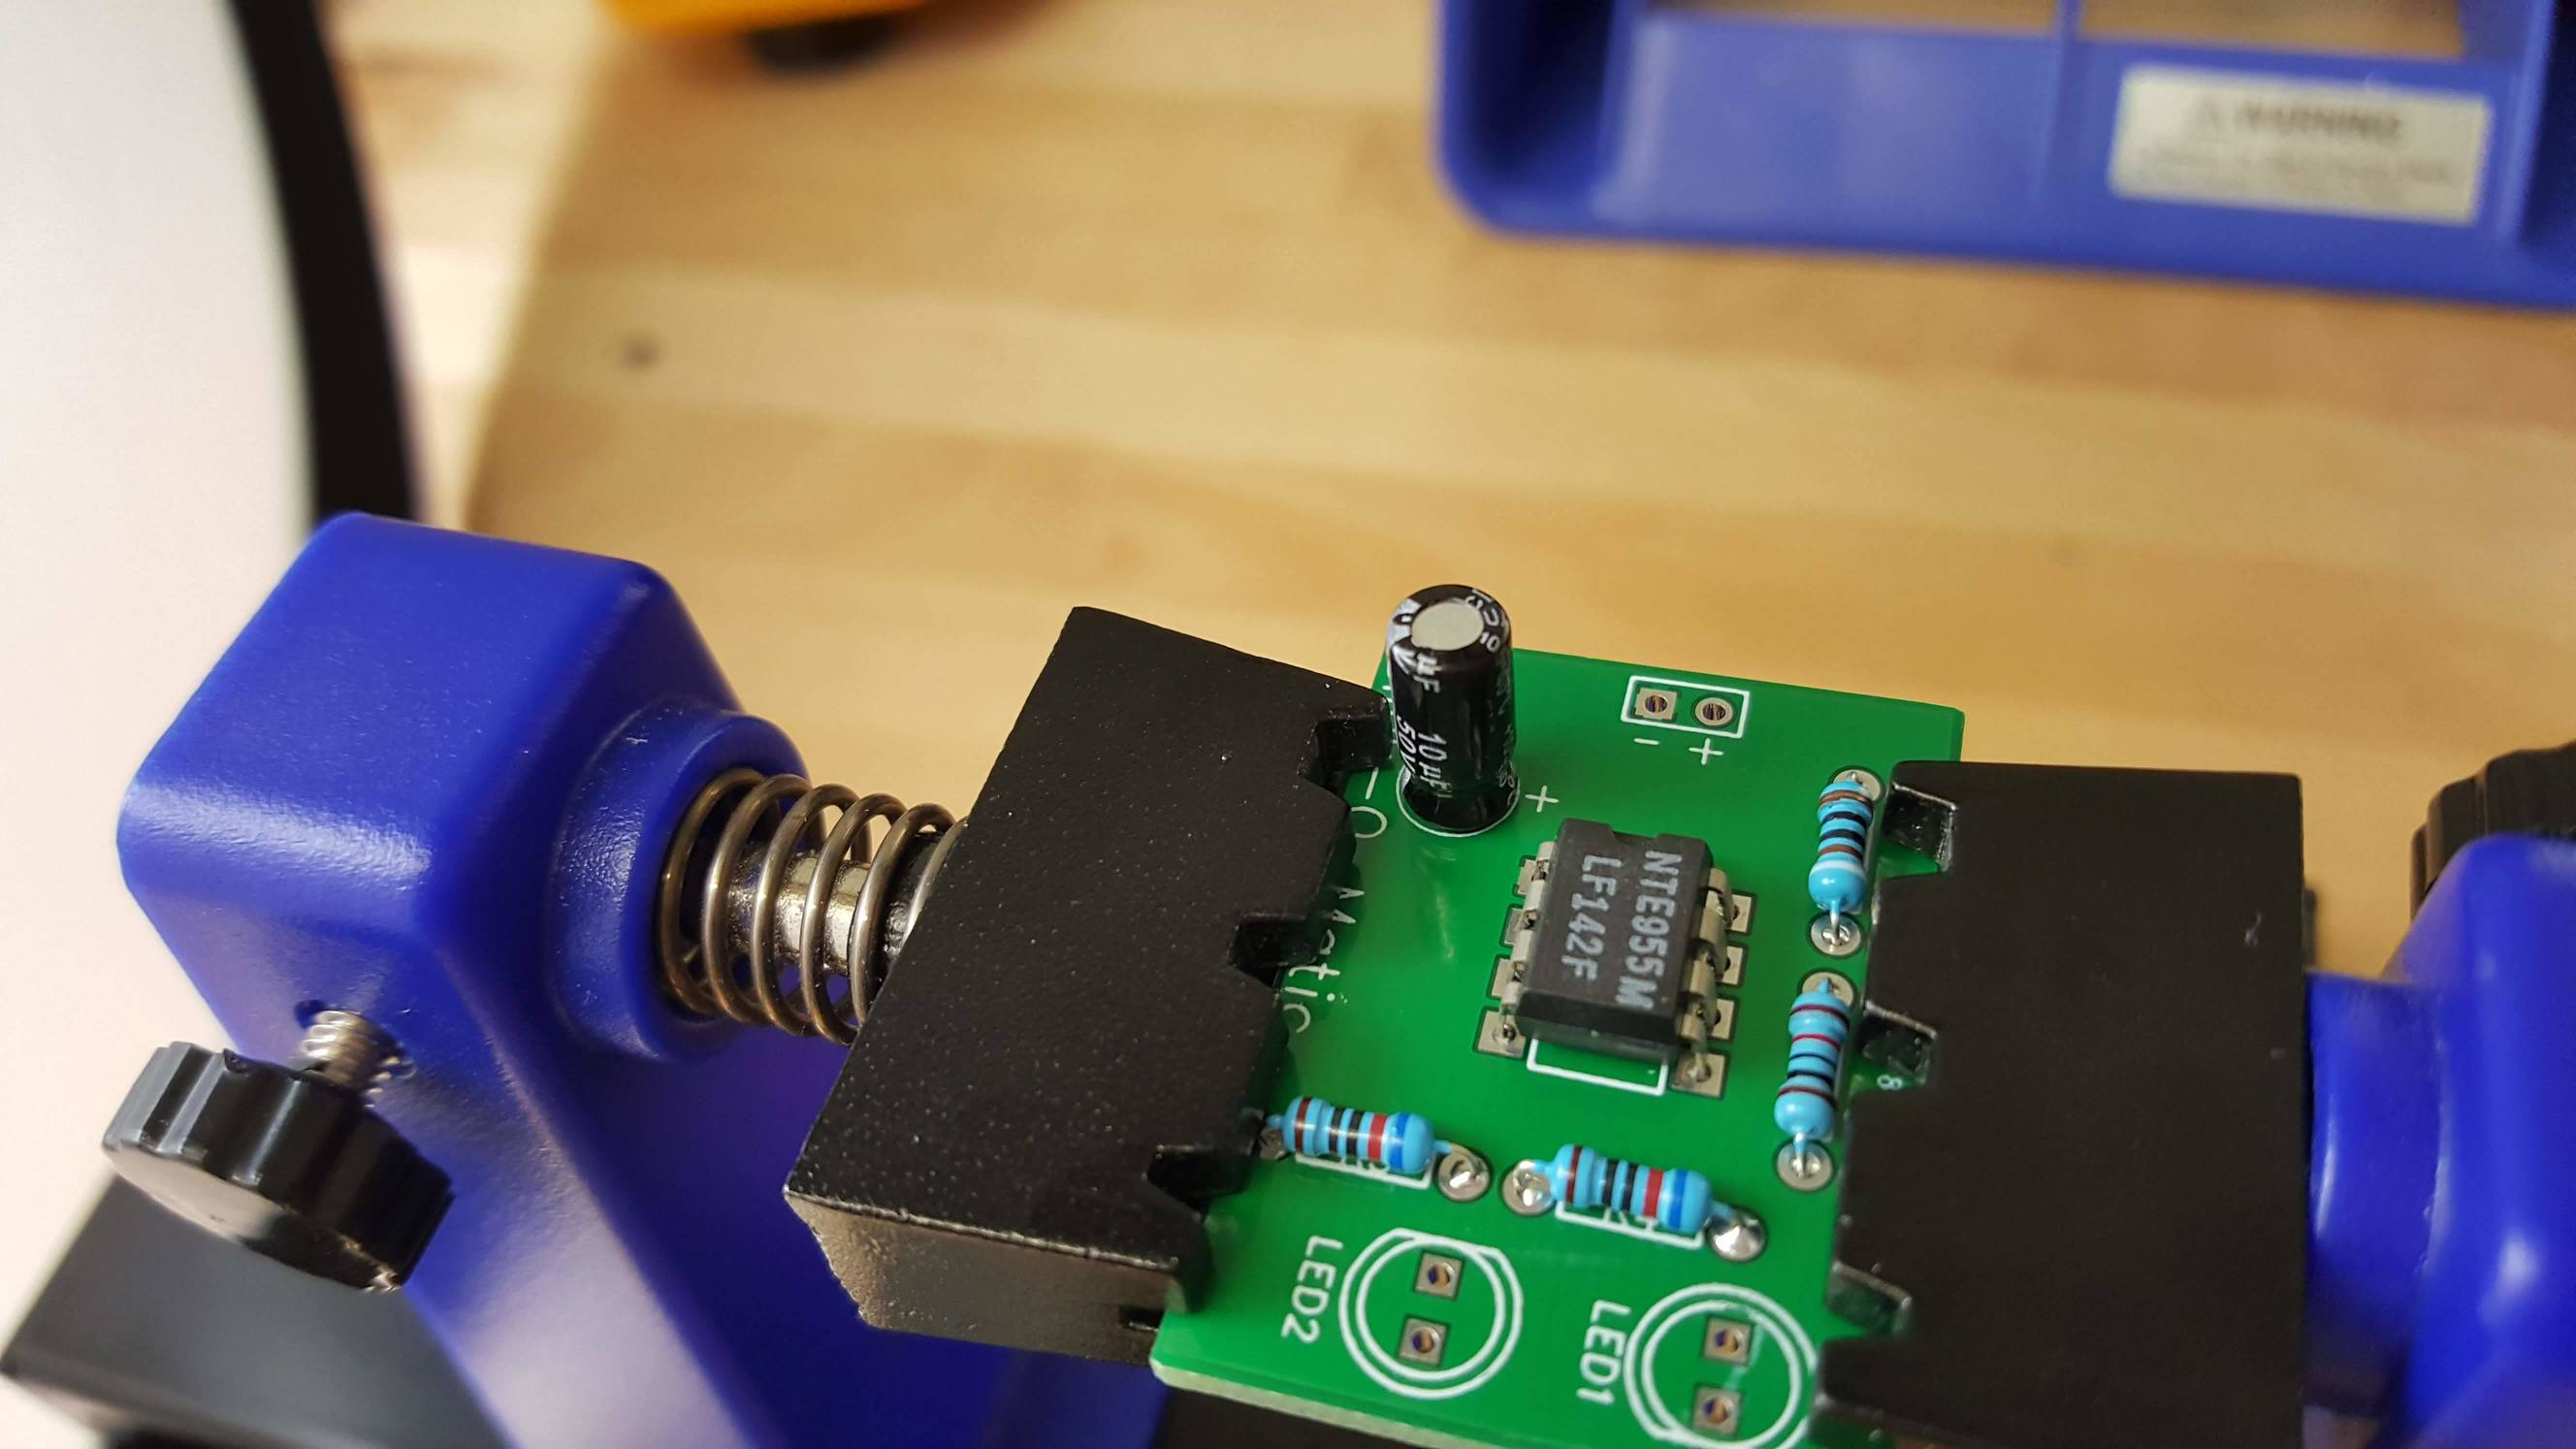
\includegraphics[width=0.75\textwidth]{img/0041.jpg}
\end{figure}

      
\begin{figure}[H]
\caption{ Soldering C1 }
\label{fig:img/0042.jpg}
\centering
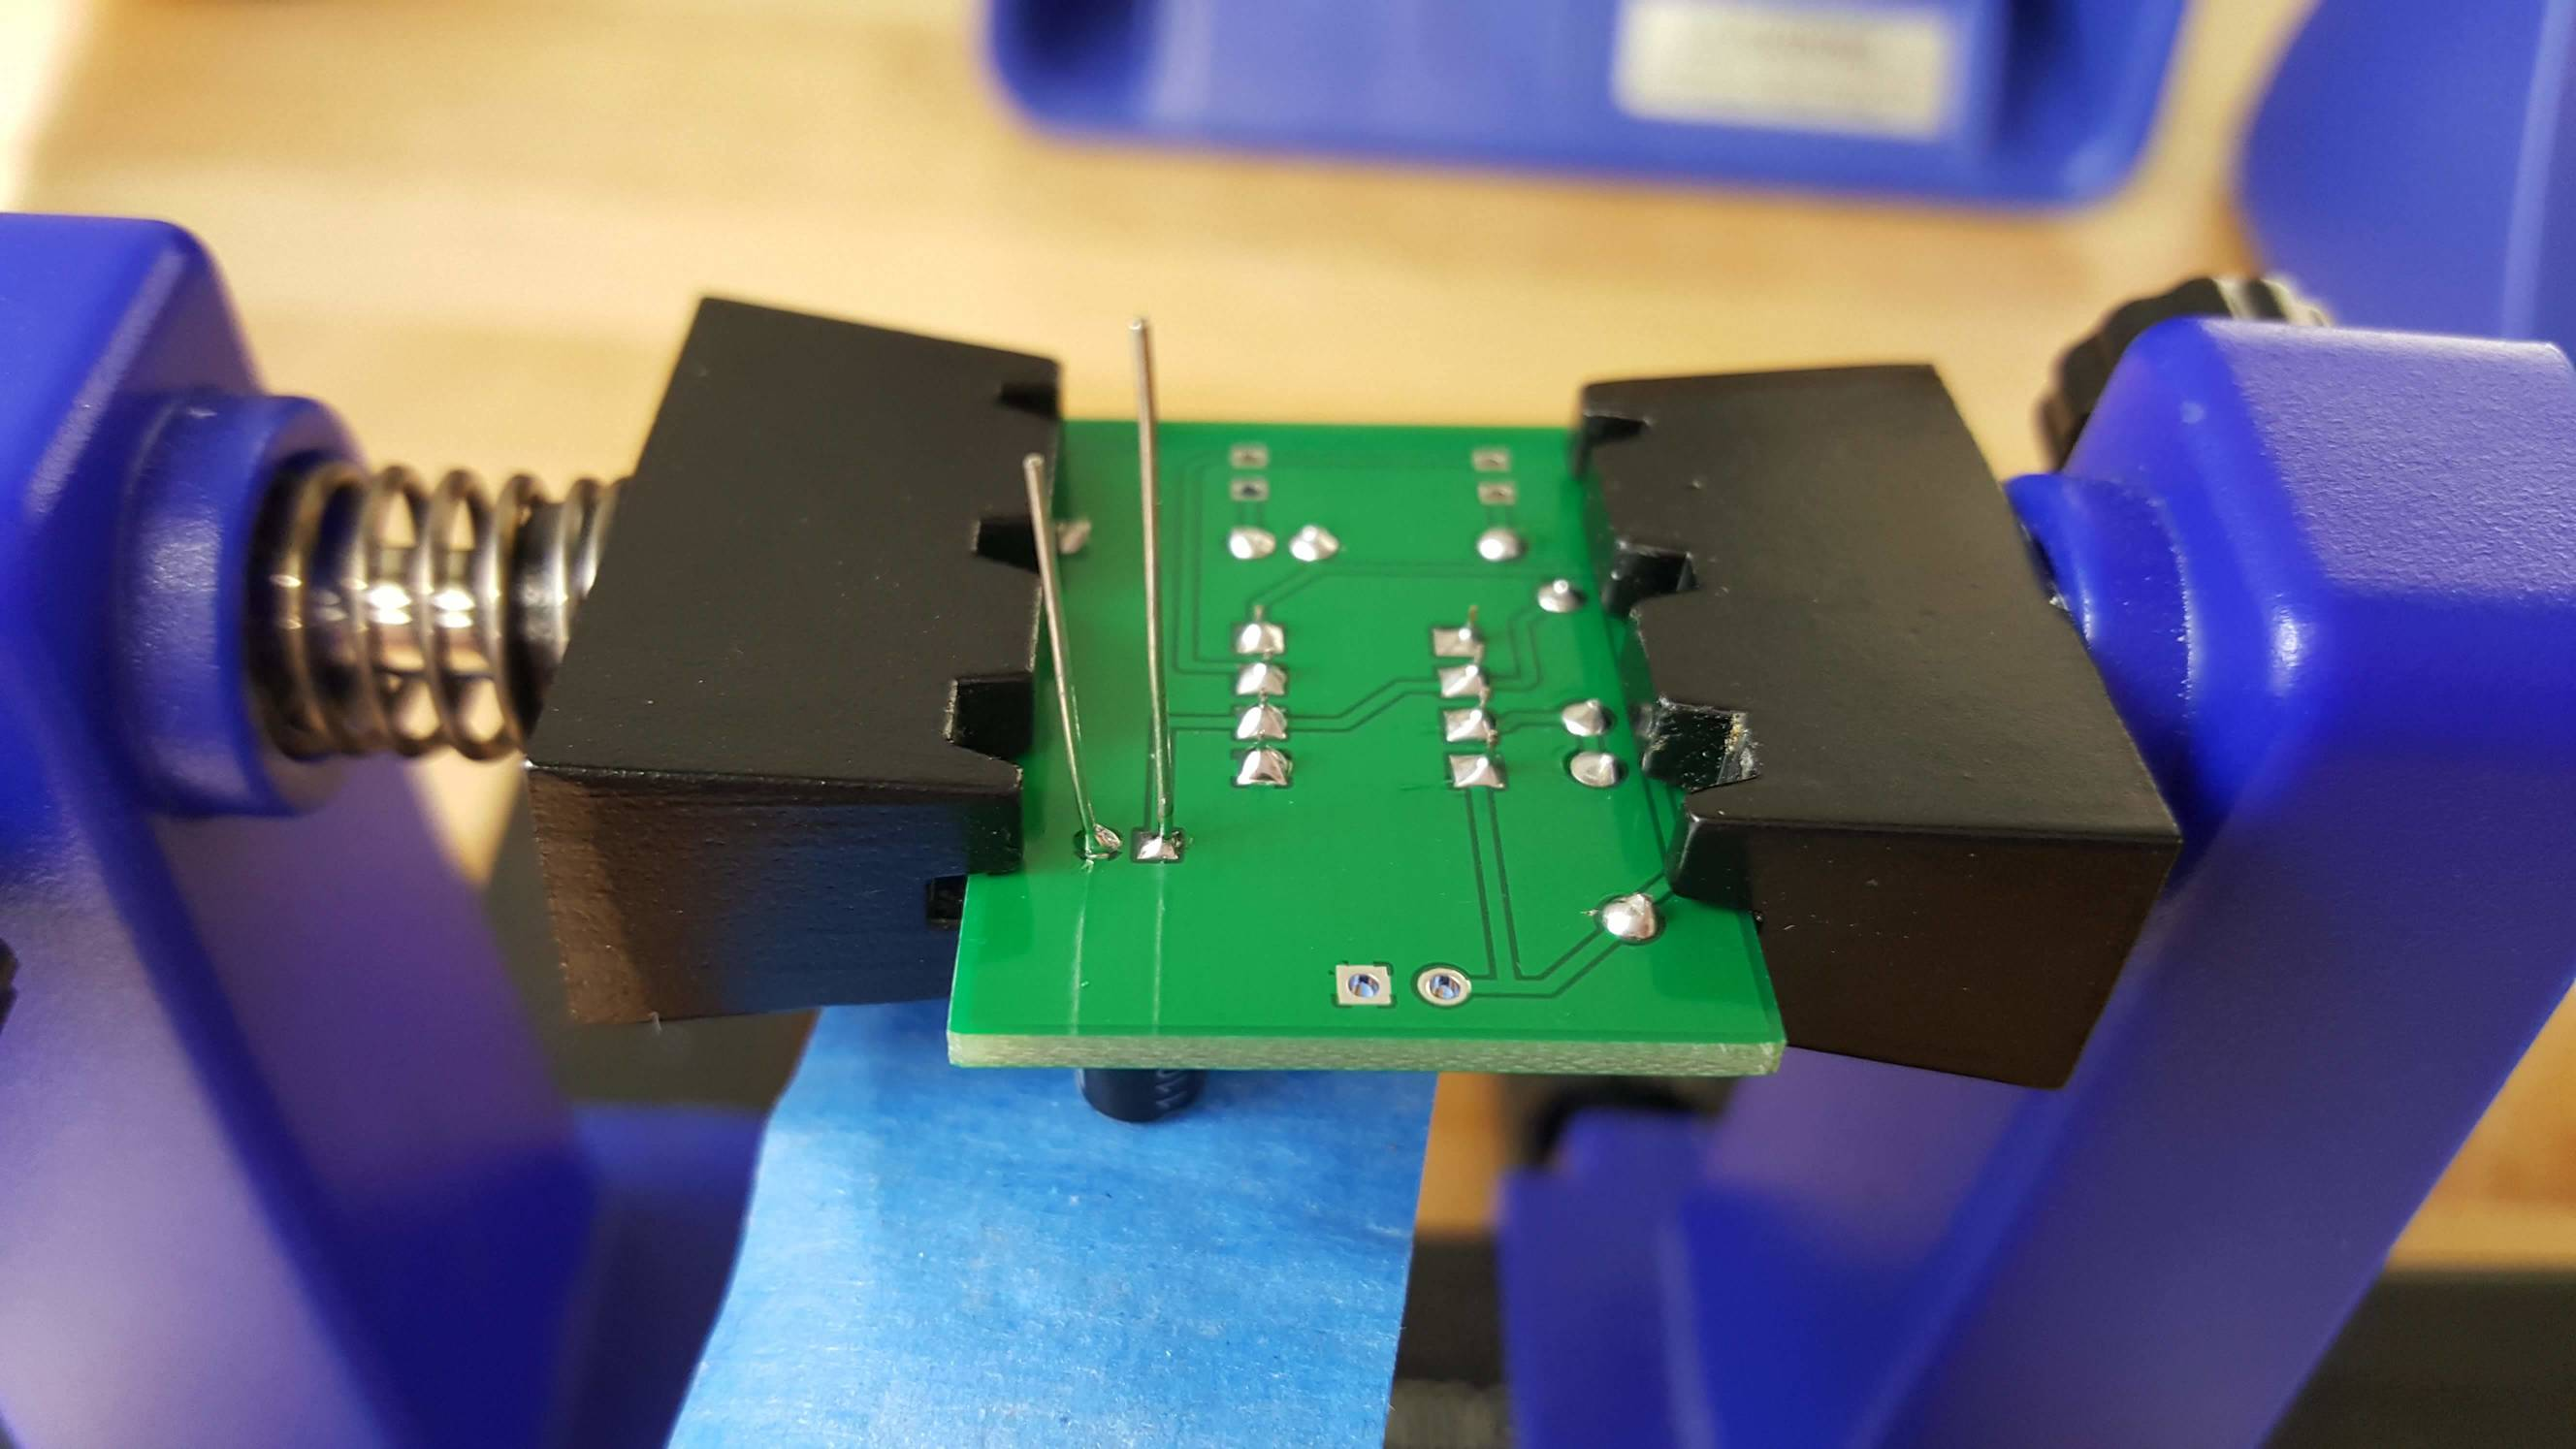
\includegraphics[width=0.75\textwidth]{img/0042.jpg}
\end{figure}

      \item 
      Next, the LED is soldered. LEDs are also polarized so their orientation matters. The LED will have a flat edge that indicates the negative lead, and the same
      longer positive lead. The circuit board has the outline of the LED, align the flat edge of the LED with the flat edge on the outline. Do this for both LEDs then solder them and
      snip their leads.
      
\begin{figure}[H]
\caption{ LED (note the flat side indicating negative and longer positive lead) }
\label{fig:img/0043.jpg}
\centering
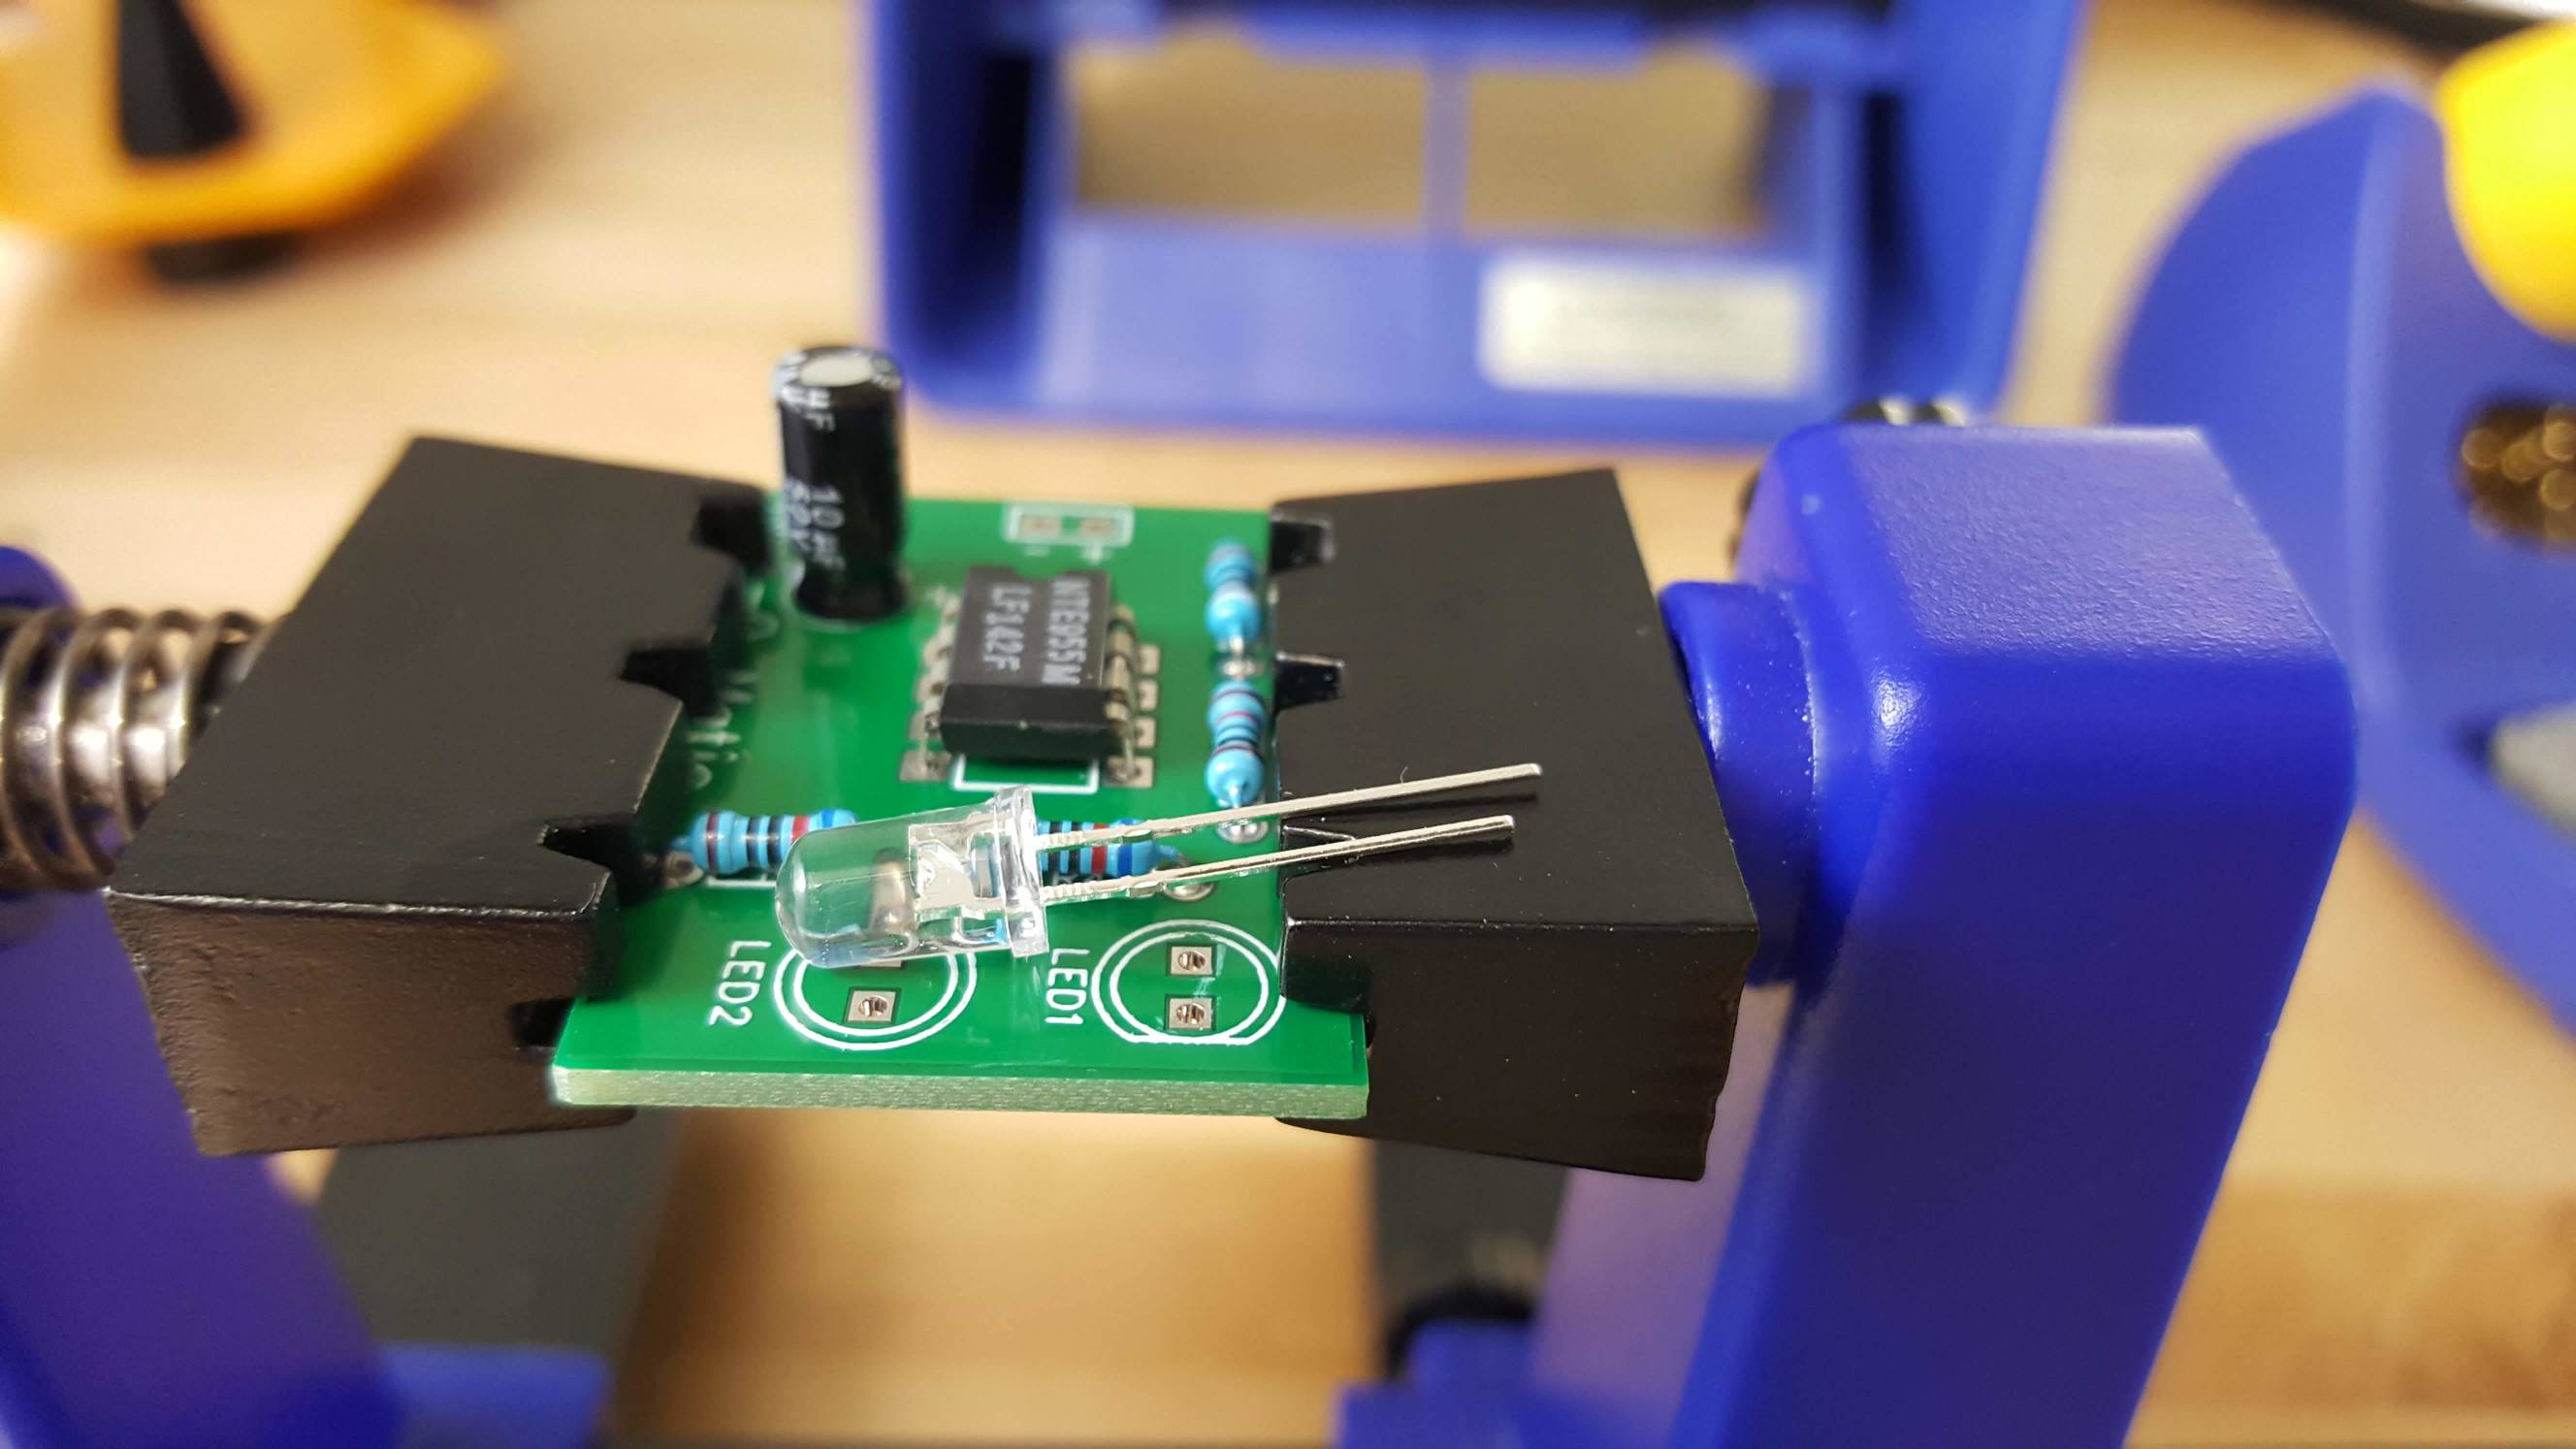
\includegraphics[width=0.75\textwidth]{img/0043.jpg}
\end{figure}

      
\begin{figure}[H]
\caption{ Inserting LED (being careful of polarity) }
\label{fig:img/0045.jpg}
\centering
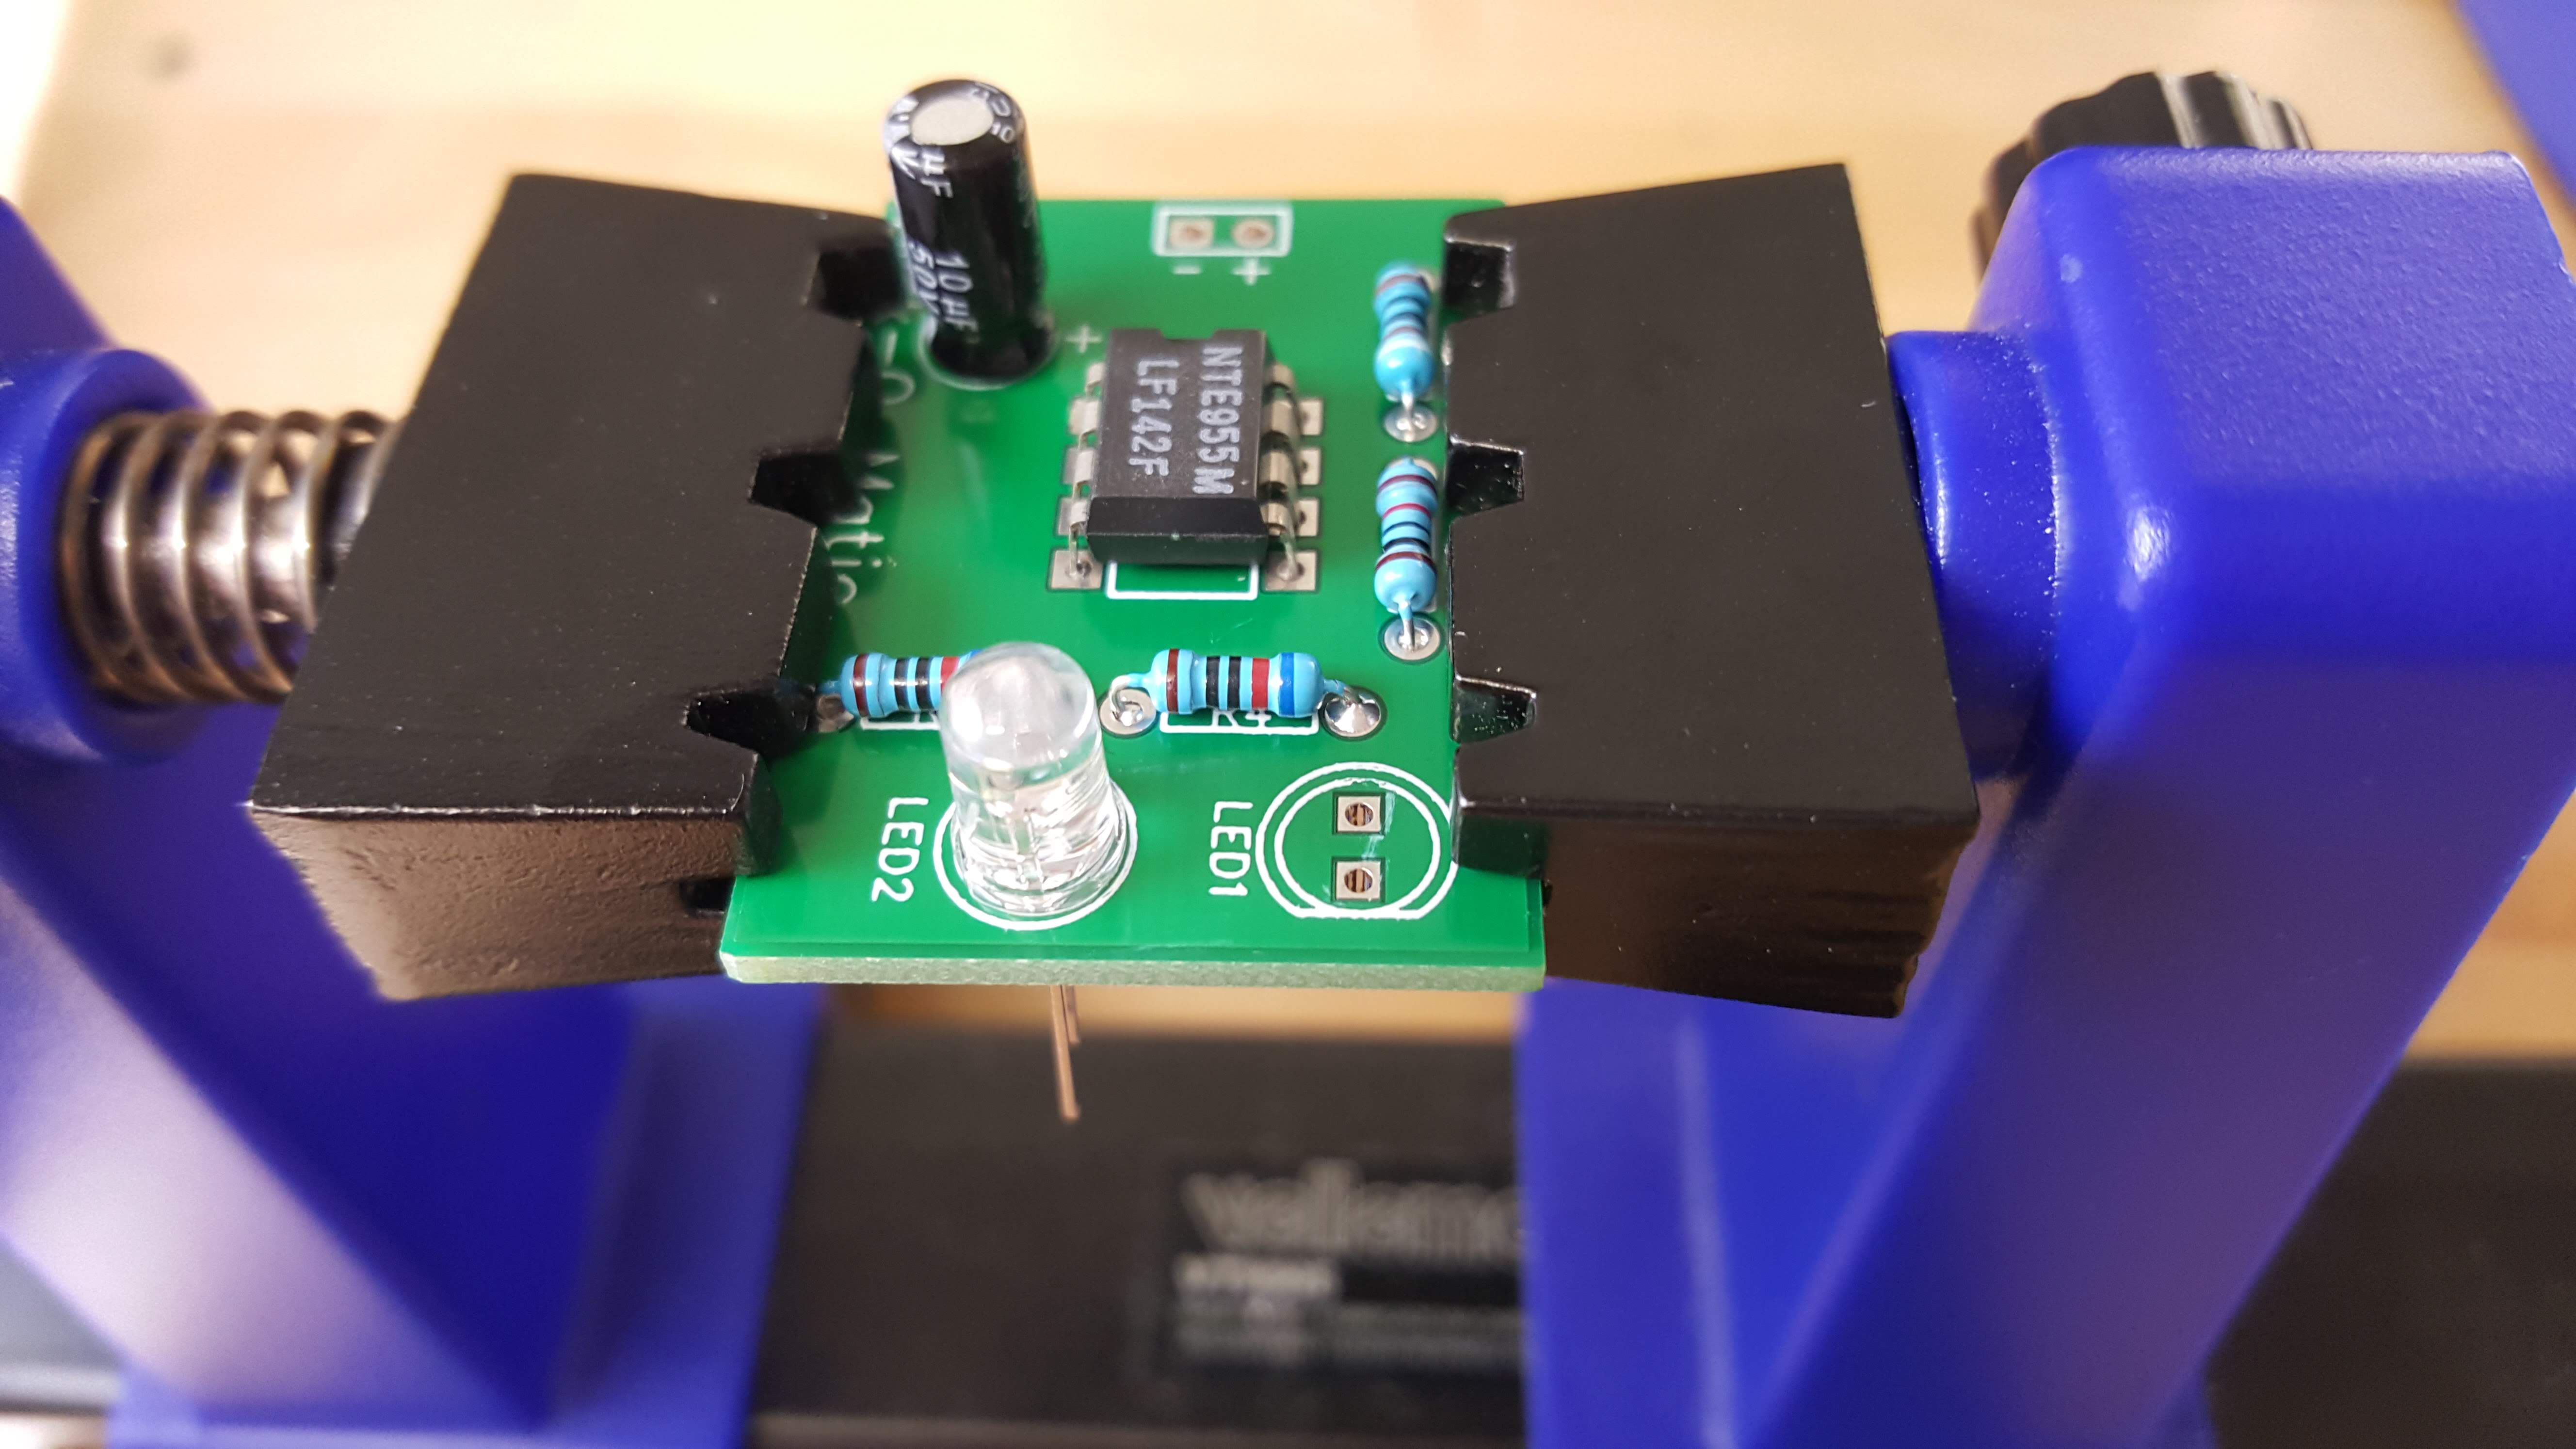
\includegraphics[width=0.75\textwidth]{img/0045.jpg}
\end{figure}


      
\begin{figure}[H]
\caption{ Both LEDs in Place (they are oriented opposite from each other) }
\label{fig:img/0046.jpg}
\centering
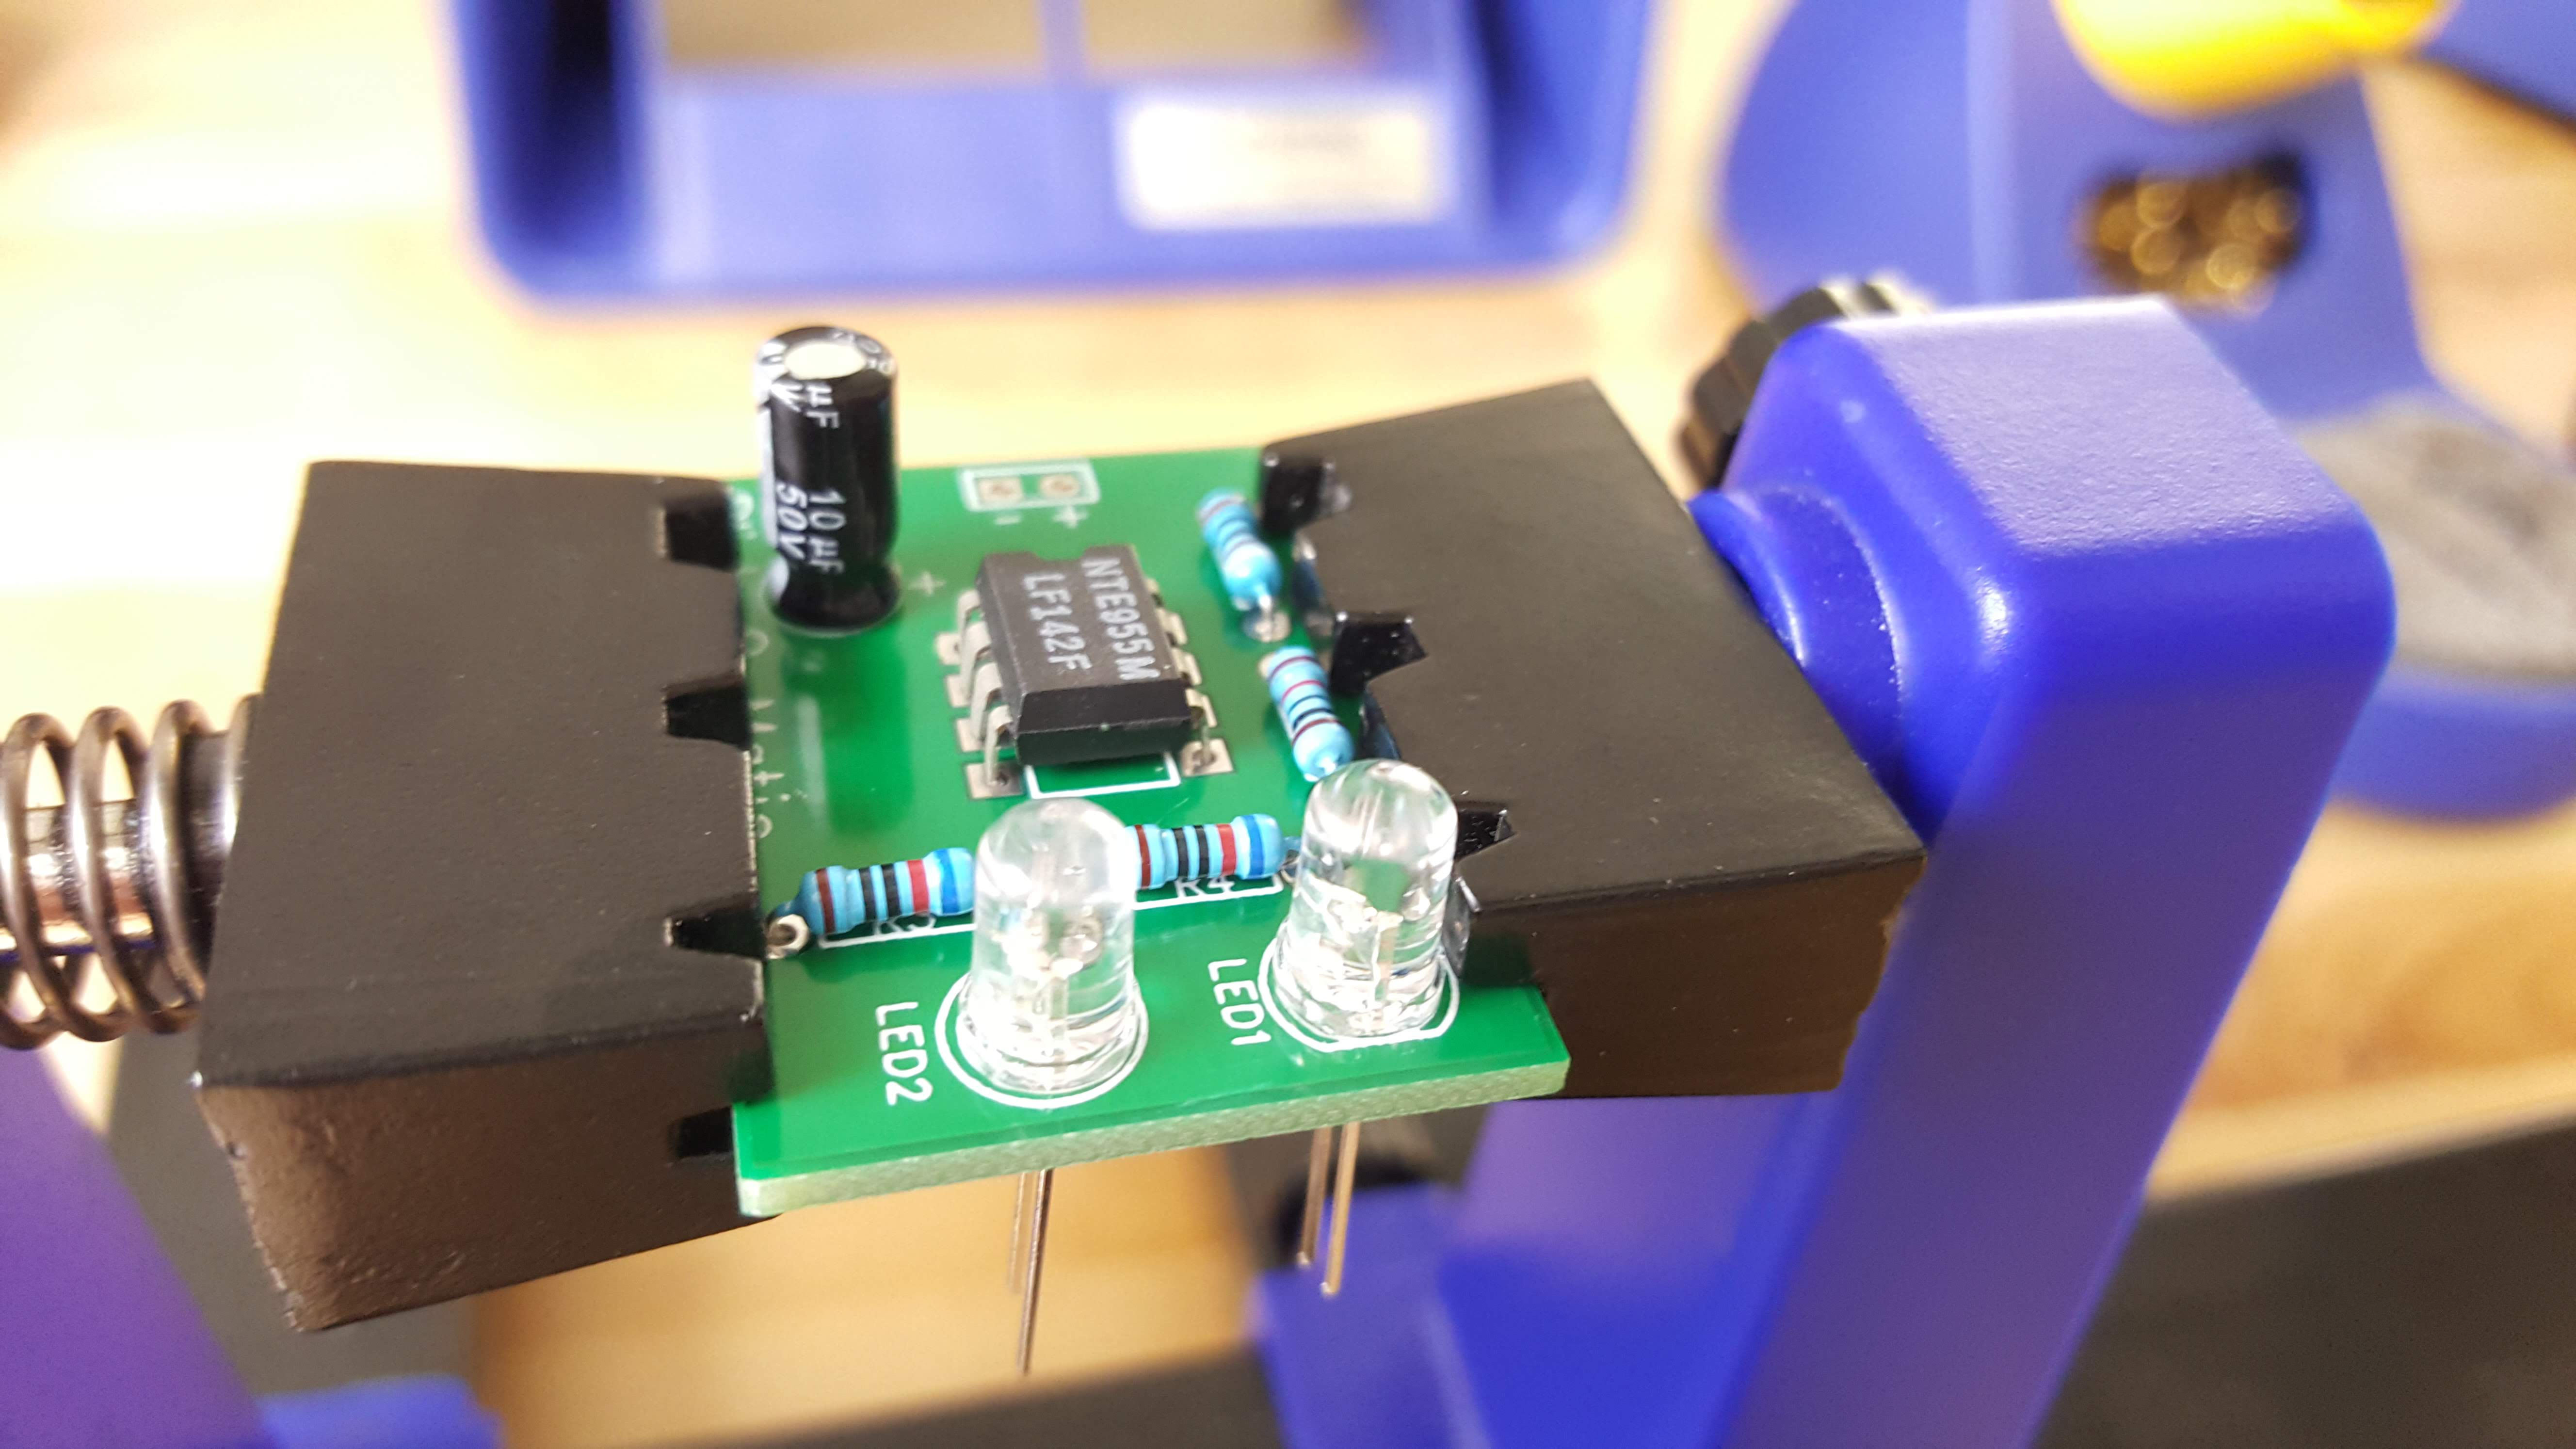
\includegraphics[width=0.75\textwidth]{img/0046.jpg}
\end{figure}

      
\begin{figure}[H]
\caption{ Both LEDs Soldered }
\label{fig:img/0047.jpg}
\centering
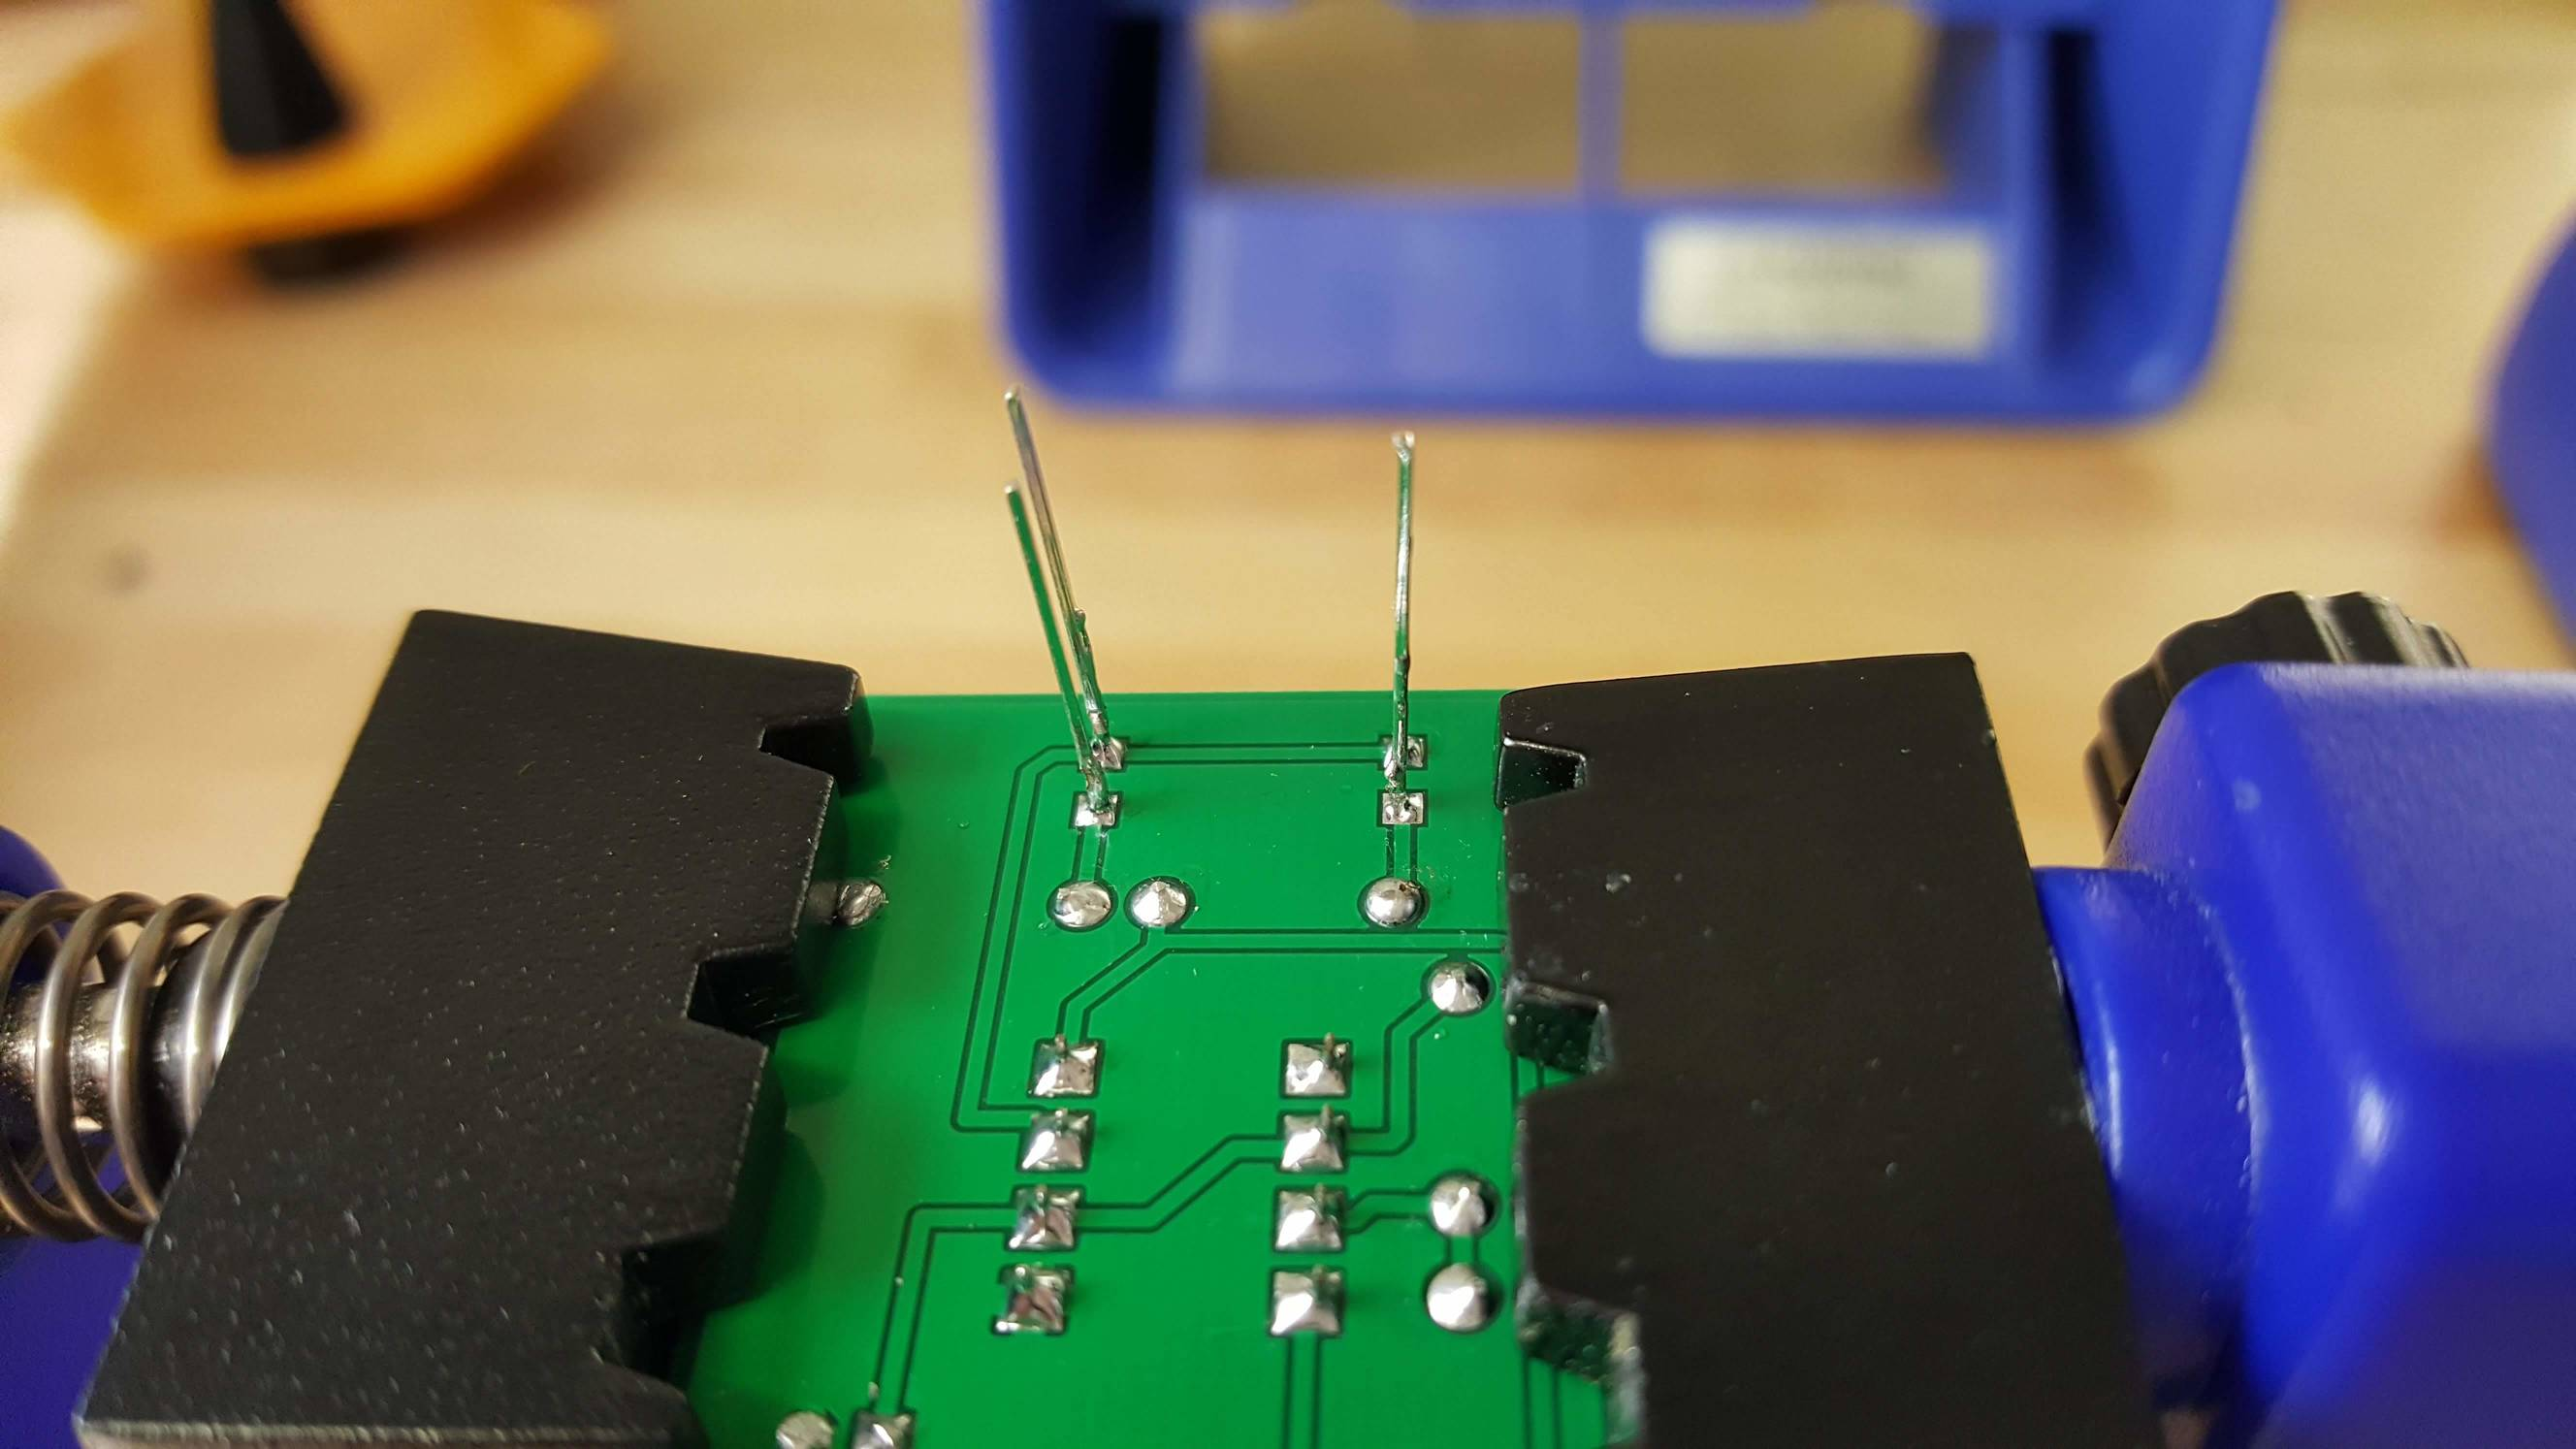
\includegraphics[width=0.75\textwidth]{img/0047.jpg}
\end{figure}

      \item  Finally, The 9V battery snap is soldered. Insert the red wire into the hole labeled with the plus sign, and the black to the one
      with the negative sign. Solder the wires in, and then snip the leads.
      
\begin{figure}[H]
\caption{ Battery Snap Leads in place }
\label{fig:img/0048.jpg}
\centering
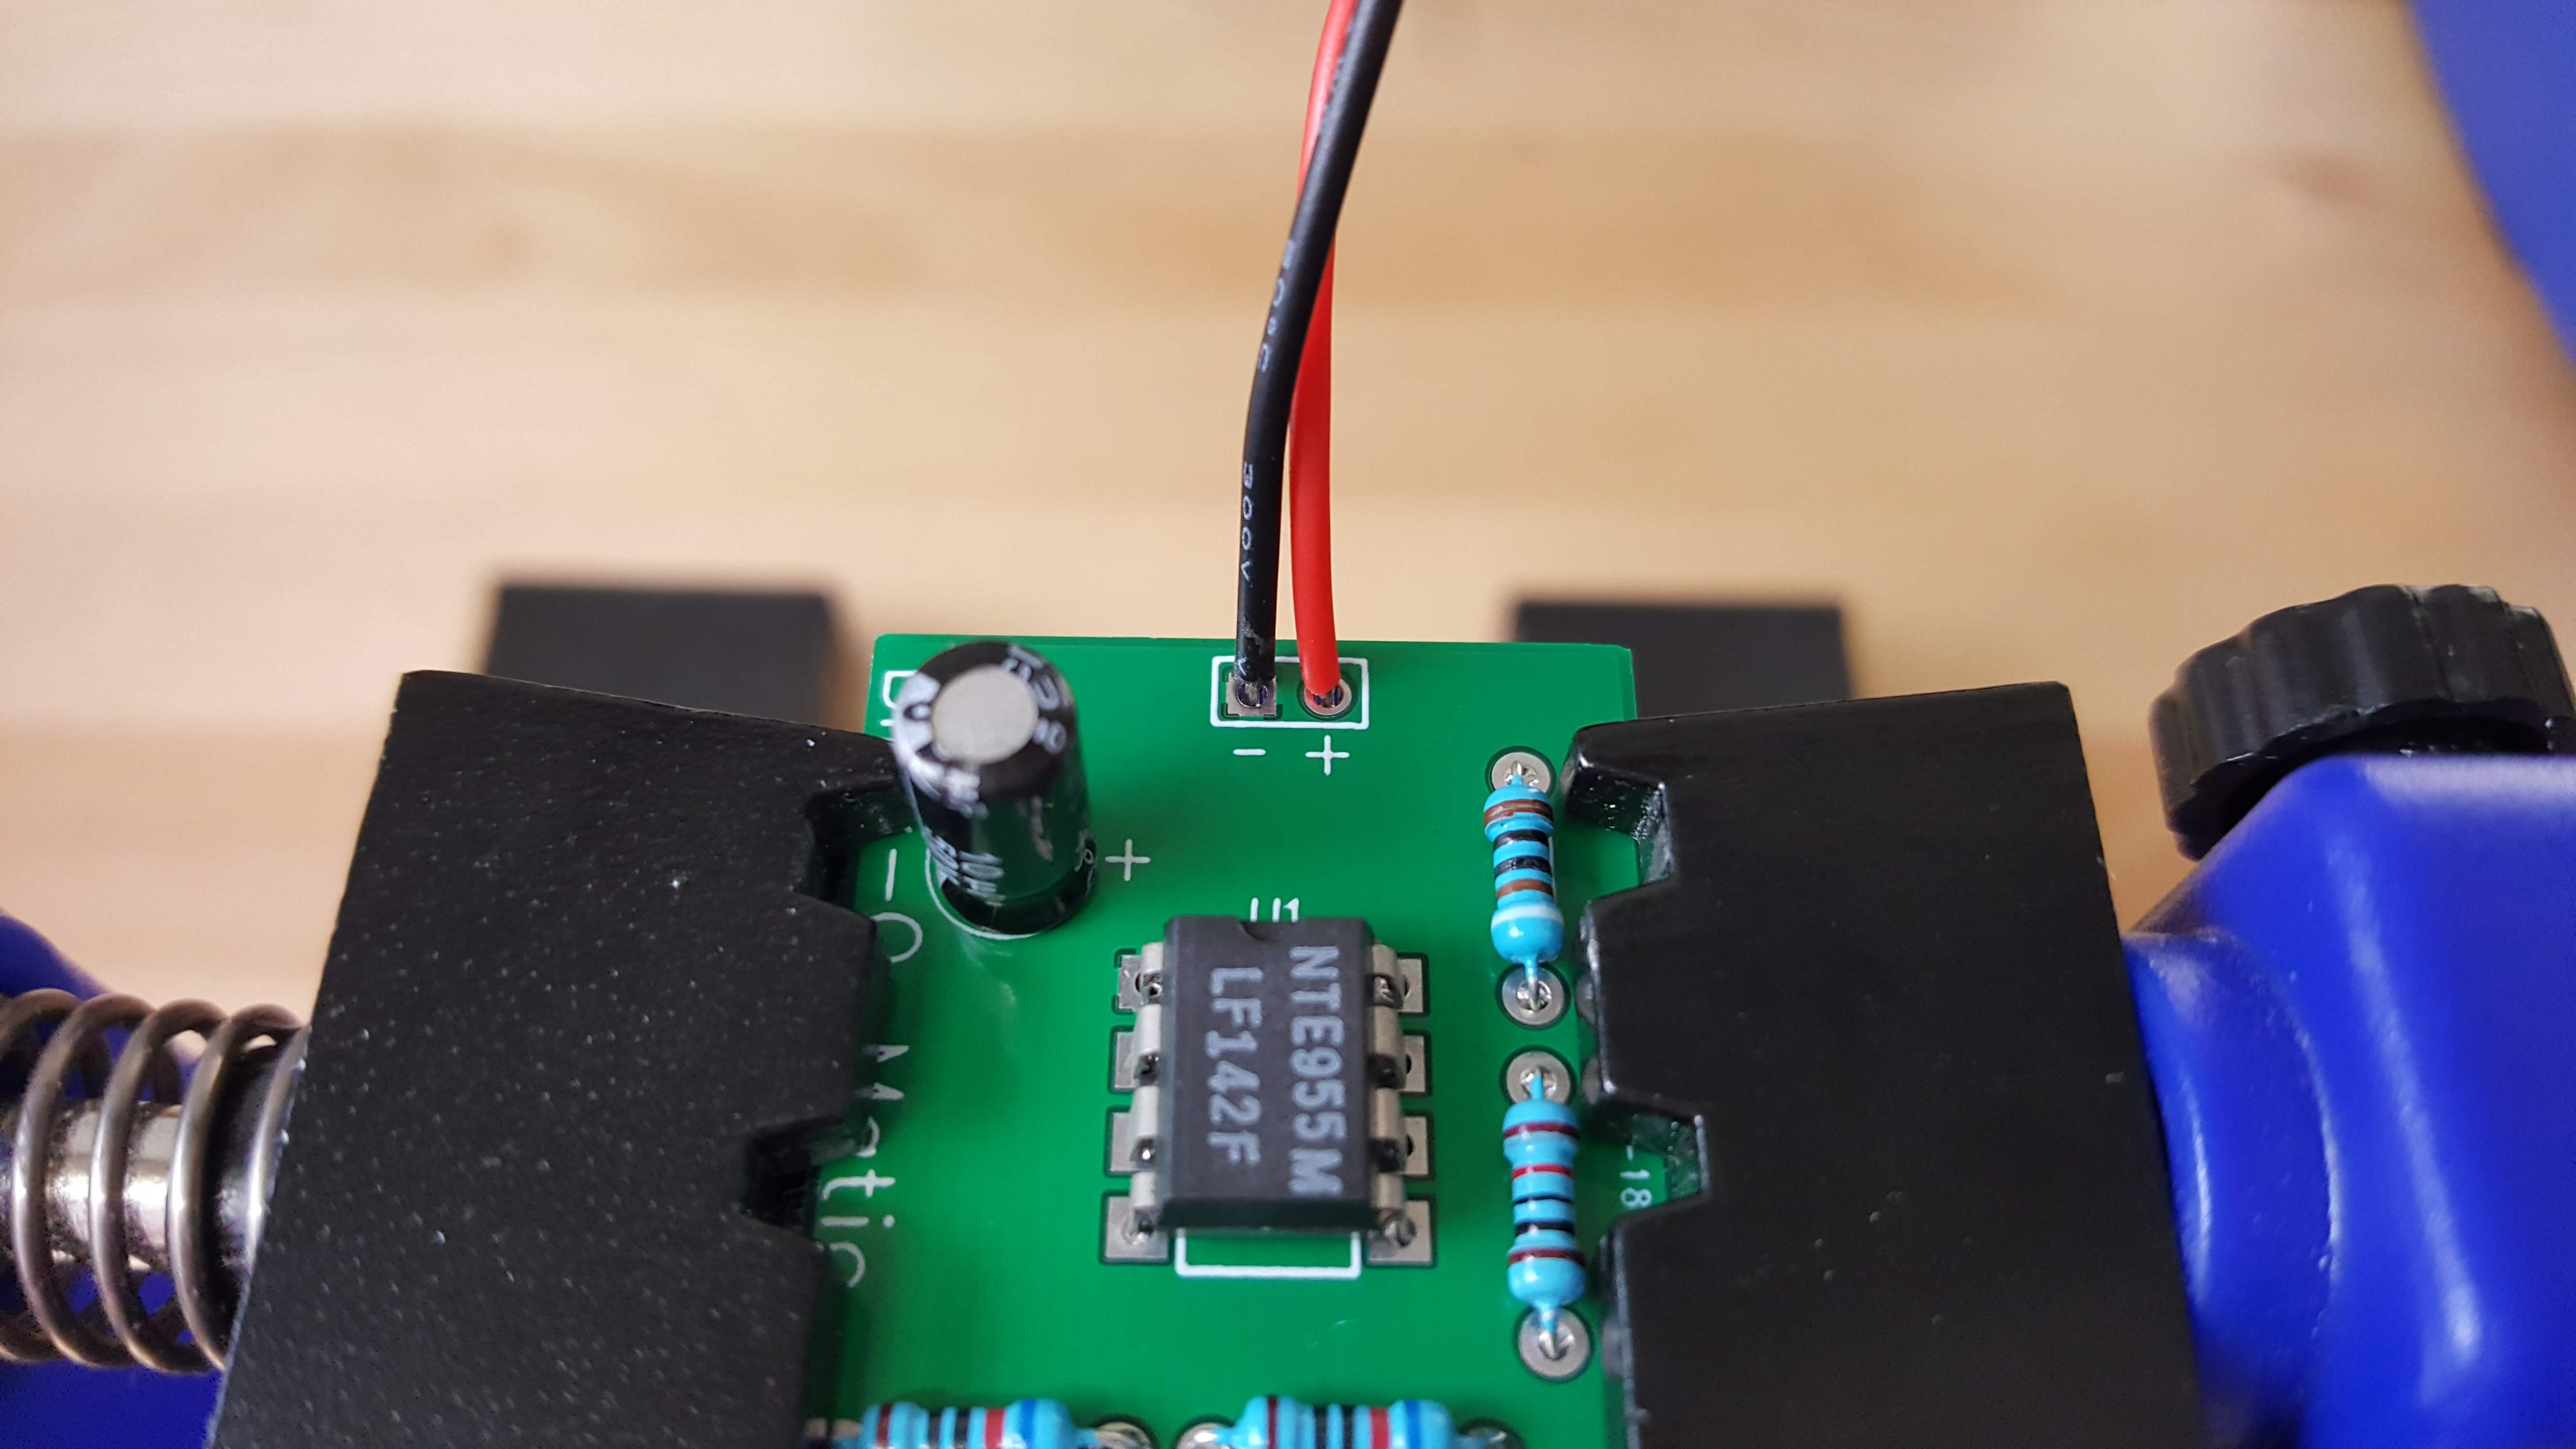
\includegraphics[width=0.75\textwidth]{img/0048.jpg}
\end{figure}

      
\begin{figure}[H]
\caption{ Battery Snap Soldered }
\label{fig:img/0050.jpg}
\centering
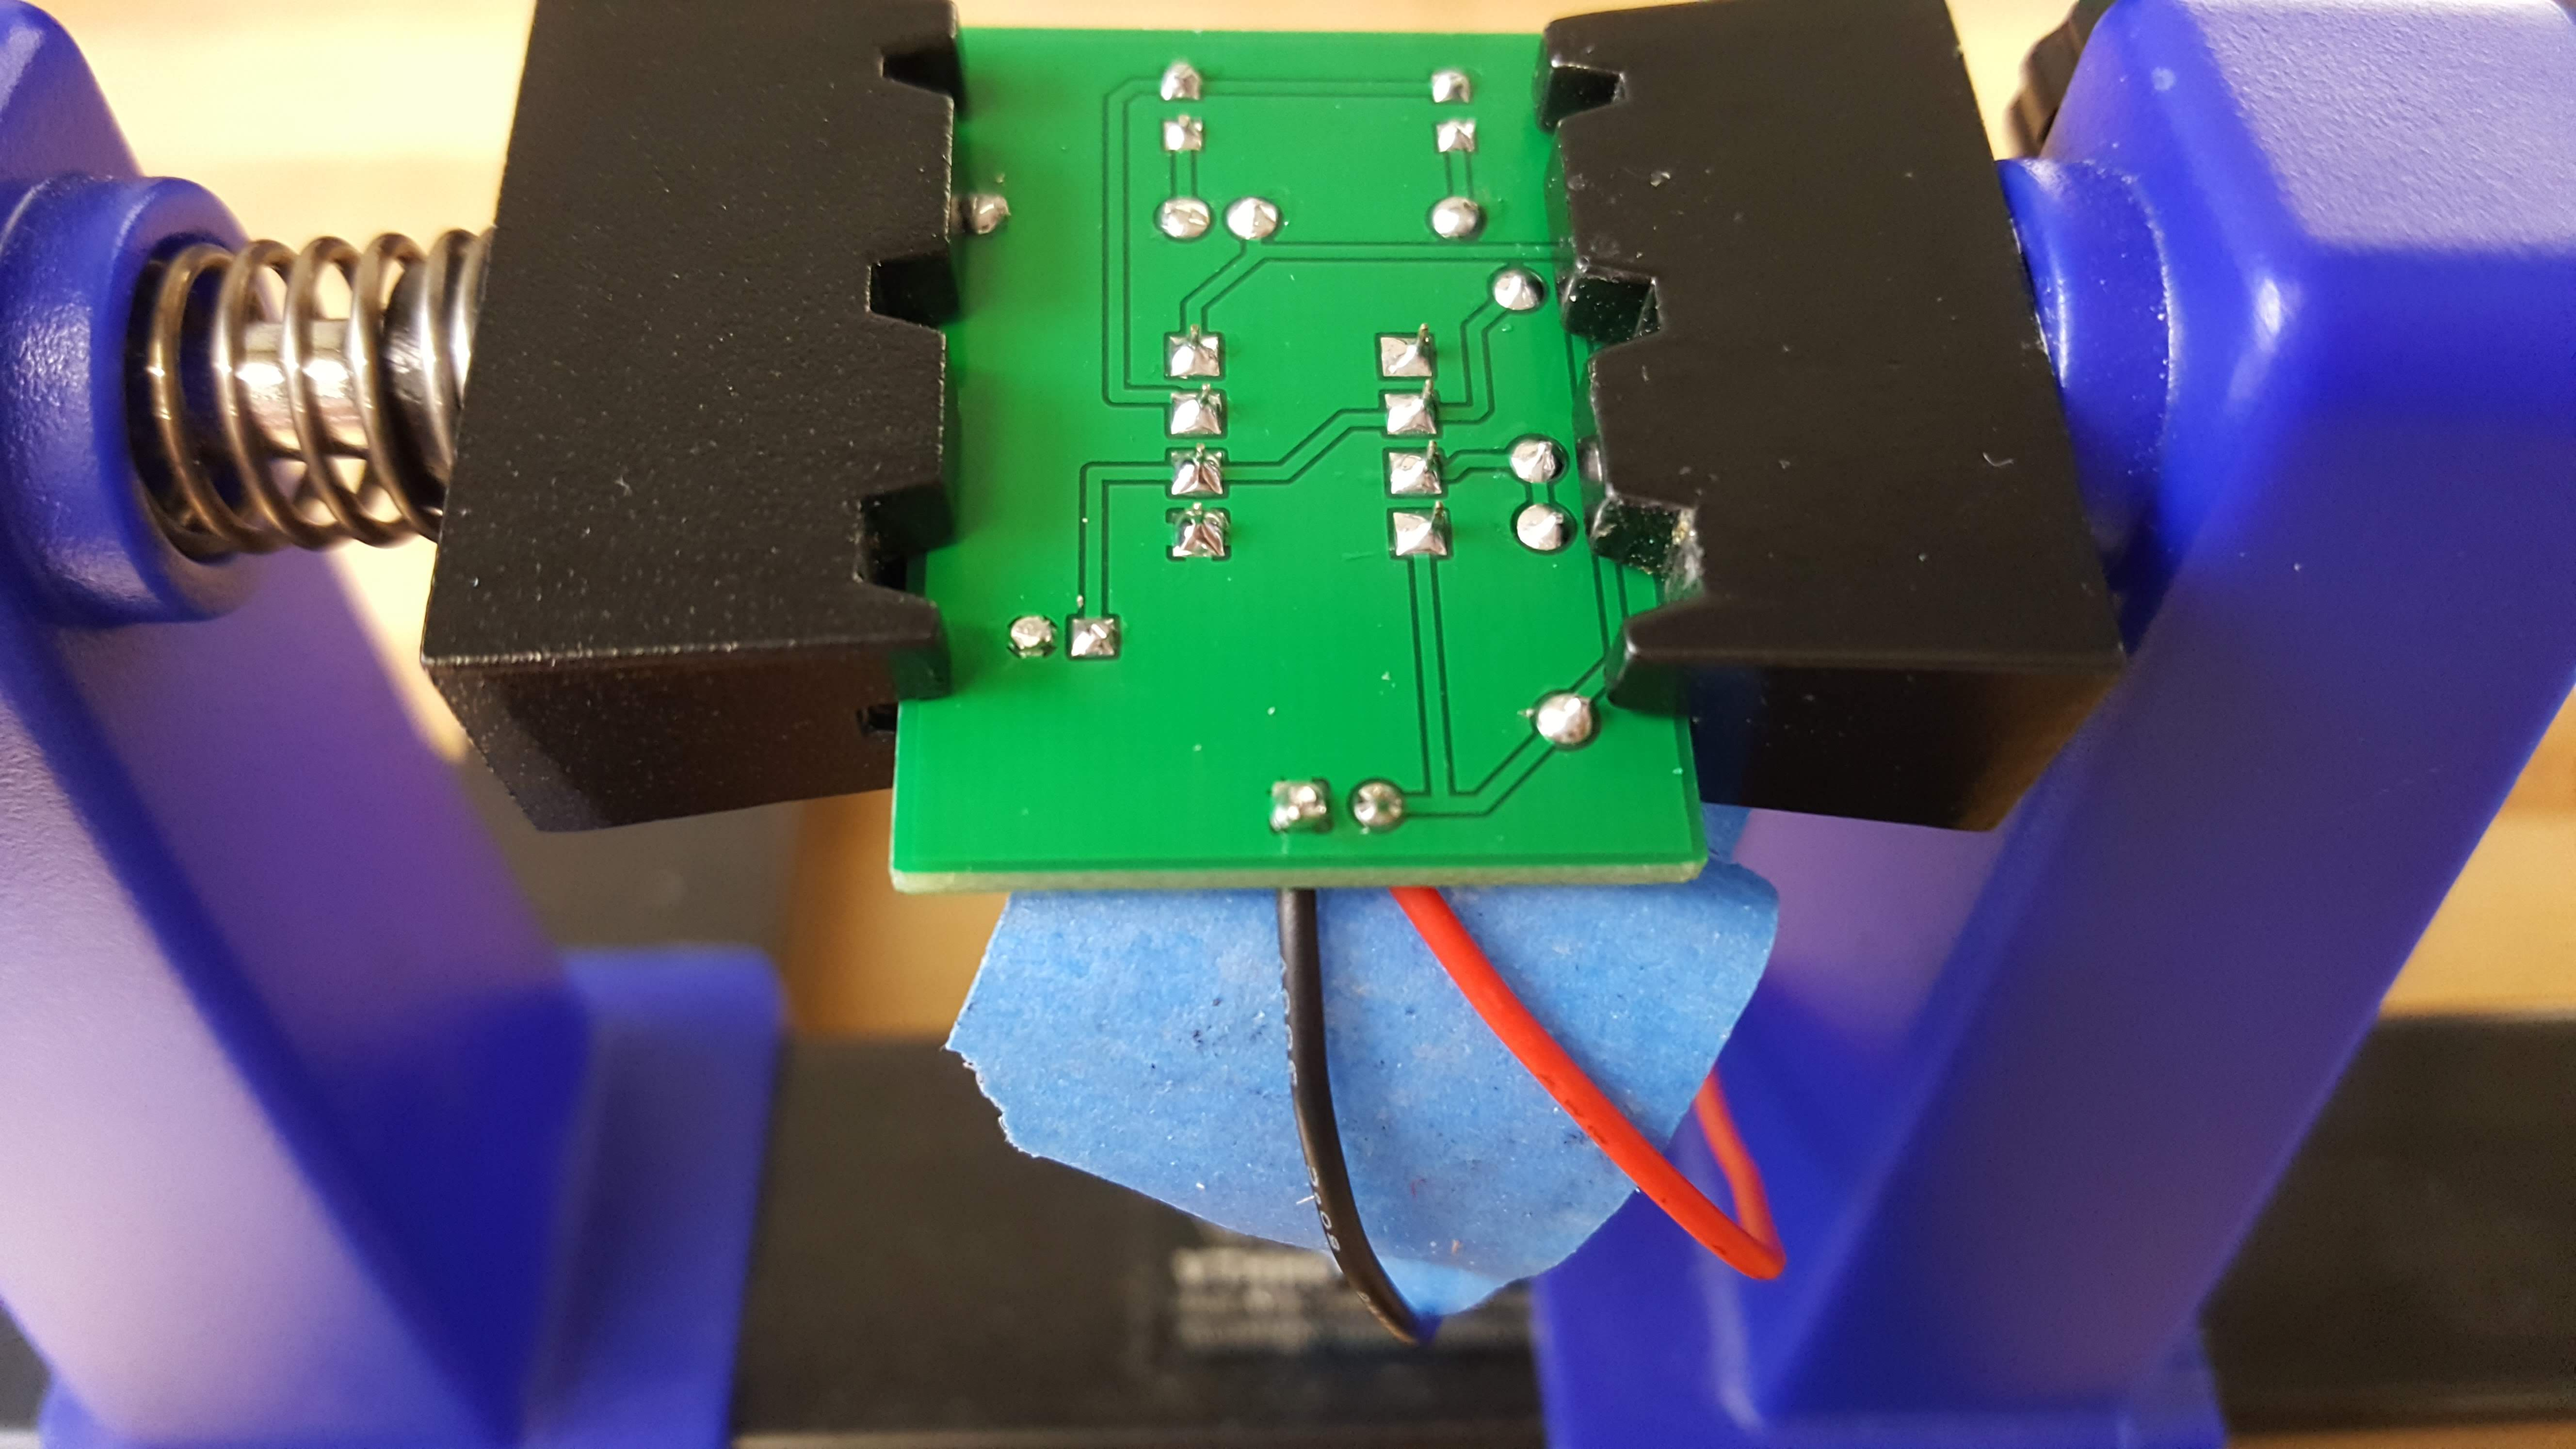
\includegraphics[width=0.75\textwidth]{img/0050.jpg}
\end{figure}

      \item 
      Now the kit is finished and can be powered with a 9v battery.
      
\begin{figure}[H]
\caption{ Finished Kit }
\label{fig:img/0052.jpg}
\centering
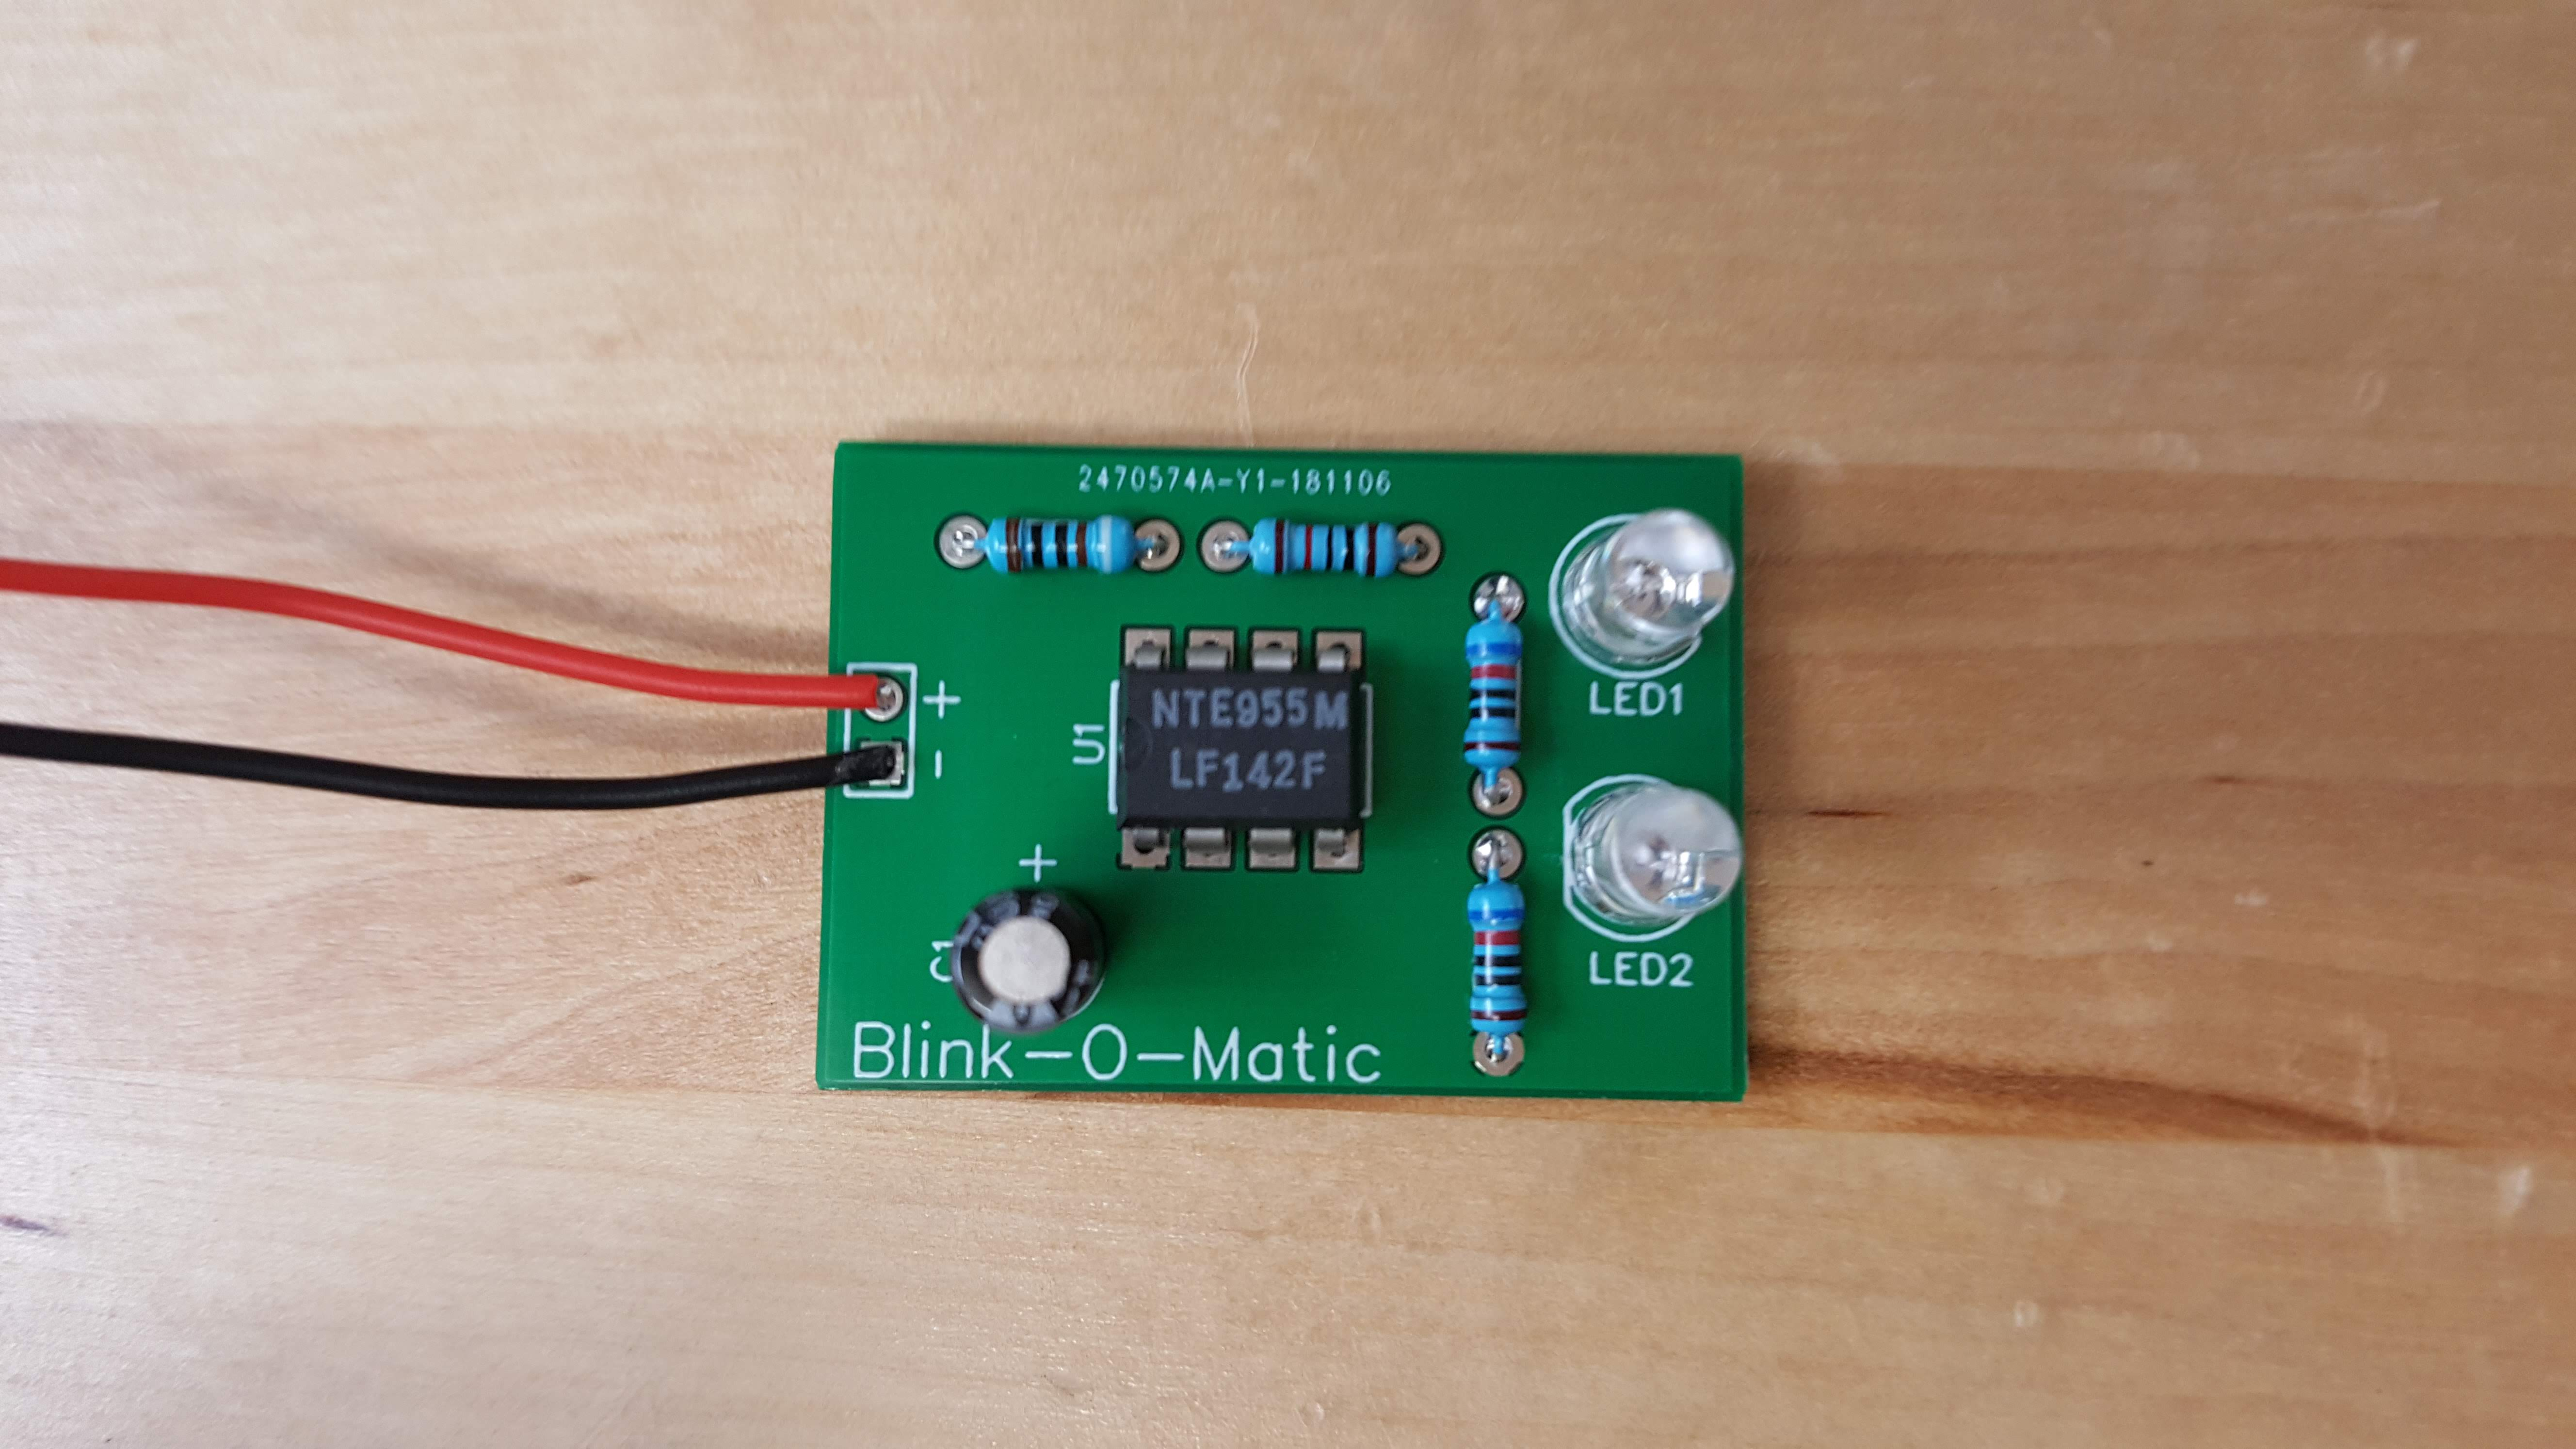
\includegraphics[width=0.75\textwidth]{img/0052.jpg}
\end{figure}

    
  \end{enumerate}

  



    


  \end{document}


